

\documentclass{report}
\usepackage[utf8]{inputenc}
\usepackage{amsmath}
%\usepackage{algorithm}
\usepackage{listings}
%\usepackage{standalone}
%\usepackage{algpseudocode}
%\usepackage{algorithm2e}
\usepackage[linesnumbered,lined,boxed,commentsnumbered]{algorithm2e}
\usepackage{verbatim}
\usepackage{tabularx}
%\usepackage{program}
%\input{externaldoc}
%\input{verticalblock}
%\algrenewcommand\algorithmicindent{1.0em}
\usepackage{minitoc}
\usepackage{float}


\title{thesis}
\author{garniron}
\date{January 2018}

\usepackage{natbib}
\usepackage{graphicx}

\lstset{language=Fortran, morekeywords={assert}}

\newcommand{\Hij}[3][H]{\langle #2 | #1 | #3 \rangle}
\newcommand{\ket}[1]{| #1 \rangle}


\begin{document}

\dominitoc

\maketitle
\newpage

\chapter*{Acknowledgments - PROBLEMS}



Alors?? Tu n'ecris pas ta these ???


----$\mu$ VS $\ket \alpha$ pour les externes

$\ket \alpha$ au lieu de $\alpha$

probablement $N_{det}$ et $N_{gen}$

Ce qui va dans matrix dressing VS dans alpha-factory

algos dans matrix dressing au lieu de pt2

enlever $teethSize$ et en faire un simple changement de poids.

indice i+1 et j dans phasemask

permuter $N$ et $\tilde N$ ?

$f_A^B$ dans CIPSI n'est pas une "hamming" distance

Remplacer "DROP" par "BREAK" ?

mono et bi excitation c'est francais

notation "int"

changer U par V pour les sets

phase factors

\newpage

\tableofcontents
\newpage


\chapter{Introduction}

During my 3 years at the LCPQ, my work focused on improving the Quantum Package, a suit of quantum chemistry code intended for developpers. It focuses on ease of implementation and parallelism.

\chapter{Quantum Package basics}
\minitoc
\documentclass[./thesis.tex]{subfiles}

 
\begin{document}


\section{Fortran}
It us mostly based on Fortran code, a low-level, high-efficiency language popular among theoretical chemists. This facilitates use and compatibility with previously developped quantum chemsitry code, and guarantees good performances. It is natively linked to the popular LAPACK linear algebra package

\section{IRPF90}
It uses IRPF90, a metalanguage(?) build on top of Fortran, that allows a dataflow-like programming style.
IRPF90 allows create so-called "providers", which are essentially nodes of dataflow strucutres that can be used in a nearly transparent way by the user. It is fully compatible(****) with normal fotran code. Code examples will be given later... I guess... in chapter something... when it will be written.
(...ou alors exemple ici)


\section{EZFIO}


avoids cumbersome IO / serializing / etc... to an extent

EZFIO.cfg

exemple

\section{Modular structure}

It has a modular structure that allows to easily implement new methods and re-use pre-existing code.
Users can create so-called "module" for their algorithms, effectively isolating them from pre-existing code. A module can import code from other modules, but is compiled into a stand-alone executable(****). This ensures easier sharing of developped algorithms.
Typically a module is run on a specific 
(ptet exemple avec generator\_CAS versus generator\_full, mais on a pas encore parler de determinant-driven )
PSI is filtered with different function and supplied to the module using cas\_sd ( cas\_sd, mrcc ) or perturbation ( pt2 stoch )??

automatic creation of interdependent modules, with theirs own inputs and outputs ( EZFIO.cfg, discussed later ) \\
******** (ptet exemple avec generator\_CAS versus generator\_full, mais on a pas encore parler de determinant-driven >\_< PSI is filtered with different function and supplied to the module using cas\_sd ( cas\_sd, mrcc ) or full\_ci ( pt2 stoch ) )?? \\

\section{ZMQ}
More recently, it allows for easy creation of massively parallel, task-based algorithms.
Using the very flexible ZMQ library, a framework has been set up to allow users to define elementary tasks that are automatically distributed to remote nodes via TCP. Each task's result is sent back to a central, user-defined "collector". The main advantage of using TCP communication rather than the "usual" MPI implementation, is asynchronicity, flexibility in adding/removing slave nodes - and thus fault-tolerance, and the ability to use nodes through internet.


standard choice would be MPI \\
ease of use \\
flexibility in adding/removing nodes \\
... thus fault tolerance \\
asynchronicity \\
can act as a layer above MPI \\
\section{High-level task distribution - OCaml}
task "administration" is hard with low-level language such as Fortran \\
functional languages are more bug-proof \\

task "administration" is hard with low-level language such as Fortran ; but it has to be moved away from the user \\
ask him to only define a list of tasks ( as strings ), function(task) and collector(function(task)) \\
transparently distribute these tasks to remote nodes \\
template for boiler plate \\

\end{document}



\chapter{Determinant-driven approach}
\minitoc

\documentclass[./thesis.tex]{subfiles}

 
\begin{document}


\alert{ Il faut ecrire quelque part la fonction d'onde:
$$ \ket{\Psi} = \sum_I^\Ndet c_I \kI $$
et l'expression des determinants:
\begin{equation}
\begin{array}{c}
 \Psi({\bf r}_1,\dots,{\bf r}_{\Na},{\bf r}_{\Na+1},\dots,{\bf r}_N;
      \alpha_1,\dots,\alpha_{\Na},\beta_{\Na+1},\dots,\beta_N) = \\
\left|
 \begin{array}{ccc}
 \varphi_1({\bf r}_1) & \dots & \varphi_1({\bf r}_{\Na}) \\
 \vdots               & \dots &   \vdots             \\
 \varphi_{\Na}({\bf r}_1) & \dots & \varphi_{\Na}({\bf r}_{\Na}) \\
 \end{array}
\right|
\left|
 \begin{array}{ccc}
 \varphi_1({\bf r}_{\Na+1}) & \dots & \varphi_1({\bf r}_{N}) \\
 \vdots               & \dots &   \vdots             \\
 \varphi_{N_\beta}({\bf r}_{\Na+1}) & \dots & \varphi_{N_\beta}({\bf r}_{N}) \\
 \end{array}
\right|
\end{array} 
\label{eq:slater}
\end{equation}
}

Generally speaking, implementing a wavefunction method requires iteration over either two-electron integrals or determinants. \\
ease of implementation VS performances \\
ease of parallelism(?) \\
Need to explicitly maintain a list of determinant. \\




\section{Notation TBUpdated}
\begin{itemize}
	\item [$\Ne$] : Number of electrons.
	\item [$\Na$] : Number of $\alpha$-spin electrons.
	\item [$\Nb$] : Number of $\beta$-spin electrons.
	\item [$\Ndet$] : Number of determinants in the wavefunction.
	
	\item [$\Norb$] : Number of orbitals.

	\item [$\Nint$] : Number of 64-bit integers required to store $\Norb$ bits.
        $\Nint = \lfloor \frac{\Norb-1}{64} \rfloor + 1$
		
	\item [$\bitI$] : Bitstring representation of $\kI$
\begin{lstlisting}
integer*8 :: I(N_int, 2)
\end{lstlisting}
	
	\item [$\bitIsigma$] : 
	Bitstring representation of $\sigma$ spinorbitals of $\kI$, $\sigma \in \{\alpha, \beta\}$ 
\begin{lstlisting}
integer*8 :: Is(N_int)
\end{lstlisting}

	\item [ {$\bitIsigma [n] $} ] :
	Bitstring representation of $\sigma$ spinorbitals of $\kI$ in the range $[ 1+n \times 64, \min \qty (n \times 64 + 63, \Norb) ]$, $0 \leq n \leq \Nint-1 \; ;\; \sigma \in \{\alpha, \beta\}$
\begin{lstlisting}
integer*8 :: Isn
\end{lstlisting}

\end{itemize}

All the program is built such that the $\alpha$ and $\beta$ spinorbitals share the same space part. In other words, spinorbitals $i$ and $\bar{i}$ both refer to orbital $\phi_i(\br)$.


\section{Determinant internal representation}
\label{sec:det_representation}

Determinants can be written as a string of creation operators applying to the vacuum state $\vac$.
$$\ac{i} \ac{j} \ac{k} \vac = \hat{I} \vac = \kI$$
Because of the fermionic nature of electrons, permutation of two contiguous creation operators results in a sign change, which makes their ordering relevant.
$$\ac{j} \ac{i} = -\ac{i} \ac{j}$$
$$\ac{j} \ac{i} \ac{k} \vac = -\kI$$
This effectively allows to make any $\Nperm$ permutations (even of non-contiguous operators), and always get
$$-1^{\Nperm} \kI$$


We see a determinant can be broken down into two pieces of information:
\begin{itemize}
\item
An unordered set of creation operators. Essentially, the set of occupied spinorbitals.
\item
A sign, the so-called \emph{phase factor}, indicating whether the creation operators are ordered so as to refer to $\kI$ or $-\kI$.
\end{itemize}

Determinants are always associated with a coefficient, so we don't need to make the phase factor part of a determinant's internal representation ; the sign will simply be reported on the associated coefficient. Still, we have to make unambiguous to what exact determinant this coefficient applies to, so we need to define an ordering to which our ``phaseless'' representation implicitly refers. We choose the order where all the $\alpha$ spinorbitals are placed before the $\beta$ spinorbitals:
\begin{equation}
\label{eq:spinpack}
\hat{I} \vac = \hat{I}_\alpha \hat{I}_\beta \vac = \kI
\end{equation}
and within each operator $\hat{I}_\alpha$ and $\hat{I}_\beta$, the creation operators are sorted with
increasing indices.
For instance, the determinant built from the set of spinorbitals $\{\bar i, i,j,k \}$ with $j>i$ and $k>j$ is
$$\kJ = \ac{i} \ac{j} \ac{k} \ac{\bar i} \vac $$
So if we happen to build a determinant initially expressed as
$$\kJp = \ac{j} \ac{i} \ac{k} \ac{\bar i} \vac $$
it will be translated to $-\kJ$.


The occupations of the spinorbitals are stored using the so-called \emph{bitstring} encoding. A bitstring is an array of bits ; typically, the 64-bit binary representation of an integer is a bitstring of size 64.
Quite simply, the idea is to map each spinorbital to a single bit, whose value is set to its occupation number. In other words \texttt{0} and \texttt{1} are associated with the \emph{unoccupied} and \emph{occupied} states.
By this definition, bitstrings are essentially lists of occupation numbers, which is a convenient way to
store the set of occupied spinorbitals in a determinant.

For simplicity and performance considerations, the occupations of the $\alpha$ and $\beta$ spinorbitals are stored on different bitstrings, rather than interleaved or otherwise merged in the same one. This allows to straightforwardly map orbital index $n$ to bit index $n-1$ (orbitals are usually indexed from $1$, while bits are indexed from $0$), and makes a bitstring a set of orbitals.
This makes the representation of a determinant a tuple of two bitstrings, associated with respectively $\alpha$ and $\beta$ spinorbitals. Such objects are refered to as \emph{$\alpha \beta$-bitstrings}, and generally define a set of spinorbitals. When used to define a determinant, they imply the previously defined ordering.


\begin{itemize}
\item
$\bitI$ is the $\alpha \beta$-bitstring representation of $\kI$
\item
$\bitI_\alpha$ is the bitstring representation of the set of occupied $\alpha$ spinorbitals of $\kI$ 
\item
$\bitI_\beta$ is the bitstring representation of the set of occupied $\beta$ spinorbitals of $\kI$ 

\end{itemize}


The storage space required for a single determinant is, in principle, one bit per spinorbital, or $2 \times \Norb$ bits. However, because CPUs are designed to handle efficiently 64-bit integers, each spin part is stored as an array of 64-bit integers, the unused space being padded with zeros. 
The actual storage needed for a determinant is
$$
2 \times 64 \times  \left \lfloor \frac{\Norb-1}{64} + 1 \right \rfloor \, \text{bits}
\label{determinantstoragespace}
$$

For a given system, we call $\Nint$ the number of 64-bits integers needed to store one spin part.
\begin{equation}
\Nint = \left \lfloor \frac{\Norb-1}{64} \right \rfloor + 1
\end{equation}


The internal Fortran representation of a bitstring is an array of $\Nint$ \lstinline{integer*8}'s (64-bit integers).

The internal Fortran representation of an $\alpha \beta$-bitstring is a two dimensional array of \lstinline{integer*8}'s, the first dimension of size $\Nint$ and the second of size $2$, corresponding to the $\alpha$ and $\beta$ spin parts.


\lstset{frame=single}
\begin{lstlisting}
  ! I is an ab-bitstring
  ! I_alpha and I_beta are bitstrings
  
  integer*8 :: I(N_int, 2)
  integer*8 :: I_alpha(N_int), I_beta(N_int)

  ... ! load some determinant in I
  I_alpha(:) = I(:,1)
  I_beta (:) = I(:,2)
\end{lstlisting}
\lstset{frame=none}


In formulas or algorithms, depending on the level of detail desired, a bitstring can be treated as a single integer of infinite size. This hides some implementation details but is unambiguous. However, in algorithms we will usually try to stay closer to the actual implementation. $\bitI$ being the $\alpha \beta$-bitstring associated with $\kI$, we can explicitly refer to a single 64-bit integer
$$\bitI_{\sigma}[i]\; ;\; \sigma \in \{\alpha, \beta\}\; ;\; i \in [0, \Nint-1]$$
which is the bitstring representation of the $\sigma$ spinorbitals of determinant $\kI$ in the range $[1+i \times 64, \min \left( (i+1) \times 64, \Norb \right)]$, indexed from $0$ to $63$.

      
\section{Bit manipulation}

The bitstring encoding is a compact way of storing determinants, but it is more than just a storage method. It allows to perform a variety of operations on determinants by taking advantage of CPU's hardware aptitude to perform efficiently bitwise operations on integers.

In many of the presented algorithms, some Fortran intrinsics will be of use. Each of those maps to a CPU instruction that is available on modern CPUs.


\begin{sloppypar}
\begin{itemize}
	      
	\item $\POPCNT{\bitI}$ :
	Returns the number of non-zero bits for a given integer $\bitI$. \\
        ${\POPCNT{\binary{00011000}} = 2}$.
	      
	\item $\TRAILZ{\bitI}$ : Returns the number of trailing zero bits for a given integer \bitI. \\
         ${\TRAILZ{\binary{00000100}} = 2}$.
	      
	      
	\item $\IBCLR{\bitI}{n}$ : Returns the value of $\bitI$ with the bit at the $n$-th position set to zero (the rightmost bit is at position zero). \\
        ${\IBCLR{\binary{00001111}}{2} = \binary{00001011}}$.
	      
	     
   	\item $\IOR{\bitI}{\bitJ}$ : Bitwise \texttt{OR} logical operation. \\
        ${\IOR{\binary{1100}}{\binary{1010}} = \binary{1110}}$.

	 
	\item $\IEOR{\bitI}{\bitJ}$ : Bitwise \texttt{XOR} (exclusive or) logical operation. \\
        ${\IEOR{\binary{1100}}{\binary{1010}} = \binary{0110}}$.
	      
	      
	\item $\IAND{\bitI}{\bitJ}$ : Bitwise \texttt{AND} logical operation. \\
        ${\IAND{\binary{1100}}{\binary{1010}} = \binary{1000}}$.
	      
	      
	\item $\NOT{\bitI}$ : Bitwise \texttt{NOT} logical operation. \\
        ${\NOT{\binary{00001100}} = \binary{11110011}}$.
	      
	\item $\ISHFT{\bitI}{n}$ : Returns $\bitI$ with bits shifted $|n|$ places to the left if $n>0$, otherwise to right. Bits shifted out of the range are lost. Zeros are shifted from the opposite end. \\
        ${\ISHFT{\binary{01001110}}{2} = \binary{00111000}}$, \\
        ${\ISHFT{\binary{01001110}}{-2} = \binary{00010011}}$.
	      
	\item $\BTEST{\bitI}{n}$ : Returns $\TRUE$ if the $n$-th bit of $\bitI$ is set, otherwise $\FALSE$. \\
        $\BTEST{\binary{00001000}}{3} = \TRUE$.
	      
\end{itemize}
\end{sloppypar}
      
      
Those intrinsics apply to integers at most 64-bits. This however is a purely implementational limitation, so depending on the level of detail desired, this constraint can be unambiguously lifted in formulas or algorithms. Different notations will be used for the 64-bit and the infinite size cases, as they are not always equivalent.
For example, the 64-bit bit-shift intrinsic always returns zero for shifts greater than 64 bits:

$$ \ISHFT{1}{n} =
\begin{cases}
2^{n}, & 0 \le n < 64 \\
0, & \text{otherwise}
\end{cases}
$$

It is convenient to introduce functions and notations acting on sets. 
More convenient notations are also desired for some operators. All binary operators are of same precedence and left-associative.

\begin{table}[H]
	\begin{tabularx}{\textwidth}{X|X}
		\hline
		
		\hline
		\rule{0pt}{3ex}
		$\ISHFT{\bitI}{n}$ & $\ishft{I}{n}$  \\ 
		
		\hline
		\rule{0pt}{3ex}
		$\TRAILZ{\bitI}$ & $\trailz{I}$  \\ 
		
		\hline
		\rule{0pt}{3ex}
		$\IBCLR{\bitI}{n}$ & $\ibclr{I}{n}$  \\ 
		
		\hline
		\rule{0pt}{3ex}
		$\BTEST{\bitI}{n}$ & $\btest{I}{n}$  \\ 
		
		\hline
		\rule{0pt}{3ex}
		$\NOT{\bitI}$ & $\neg I $  \\ 
		
		\hline
		\rule{0pt}{3ex}
		$\IAND{\bitI}{\bitJ}$ & $\iand{I}{J}$ \\
		
		\hline
		\rule{0pt}{3ex}
		$\IOR{\bitI}{\bitJ}$ & $\ior{I}{J}$ \\
		
		\hline
		\rule{0pt}{3ex}
		$\IEOR{\bitI}{\bitJ}$ & $\ieor{I}{J}$ \\
		
		\hline
		\rule{0pt}{3ex}
		$\POPCNT{\bitI}$ & $\popcnt{I}$ \\
		\hline
	\end{tabularx}
\end{table}

Note that these notations apply to integers ; whether or not they are meant to be bitstrings.

Some examples of how these instructions can be used are given below. They are key to understand how we can determine which holes and particles are created when exciting from $\kI$ to $\kJ$.
Let $\bitI$ and $\bitJ$ be the bitstring representations of $\kI$ and $\kJ$, and $\bit{P}$ a bitstring with $\Nint=1$. 


\begin{itemize}
	      
	\item $\bitx{I}{\alpha}$ : bitstring representation of the set of $\alpha$ spinorbitals of $\kI$
	            
	\item $\popcnt{\bitx{I}{\alpha}}$ : number of spinorbitals in $\bitx{I}{\alpha}$ (equal to the number of $\alpha$ electrons).
	            
	\item $\ieor{\bitx{I}{\alpha}}{\bitx{J}{\alpha}}$ : bitstring representation of the set of $\alpha$ spinorbitals that are present in either $\bitx{I}{\alpha}$ or $\bitx{J}{\alpha}$, but not in both (exclusive disjunction).
        This operator identifies the $\alpha$ spinorbitals involved in the excitation from $\kI$ to $\kJ$. 
	            
	\item $\iand{\bitx{I}{\alpha}}{\qty(\ieor{\bitx{I}{\alpha}}{\bitx{J}{\alpha}})}$ : 
        bitstring representation of the set of $\alpha$ spinorbitals of $\kI$ involved in the excitation from $\kI$ to $\kJ$. This corresponds to the indices of the holes in the excitation $\excdet{I}{J}$ or to the particles in $\excdet{J}{I}$. 
	            
	\item $\popcnt{\ieor{\bitx{I}{\alpha}}{\bitx{J}{\alpha}}}/2$ : because the excitation of an electron involves 2 spinorbitals (one hole and one particle), this is the $\alpha$ excitation degree between $\kI$ and $\kJ$.
	            
	\item $\TRAILZ{\bit{P}}+1$ : the index of the lowest orbital in $P$. If $\bit{P}$ is $0$, returns $65$.
	            
	\item $\IBCLR{\bit{P}}{\TRAILZ{P}}$ : $P$ without its orbital of lowest index.

\end{itemize}


\section{Computing Excitations}

An algorithm used to compute the excitation degree is presented as algorithm \ref{alg:EXC_DEGREE}, and one to compute the sets of created holes and particles as algorithm \ref{alg:EXC}. Algorithm \ref{alg:EXC}, however, returns the sets as bitstrings. Extracting the indices from a bitstring is another basic operation, presented as algorithm \ref{alg:LIST_FROM_BITSTRING}.
Because computing excitations is a hotspot of the program, and because we are typically interested in double excitations at most, a more specialized algorithm can be used ( PAS ENCORE ECRIT/POMPÉ ).


\begin{algorithm}[h!]
	\caption{EXC\_DEGREE}
	\label{alg:EXC_DEGREE}
	\SetKwFunction{FMain}{EXC\_DEGREE}
	\SetKwProg{Fn}{Function}{:}{}
	
	\Fn(\tcc*[h]{Computes the excitation degree between two determinants}){\FMain{$I, J$}}{
		\KwData {$I, J$ bitstring representations of determinants $\kI$ and $\kJ$}
		\KwResult{ Returns the excitation degree between $\kI$ and $\kJ$ }

		$X \gets 0$   \;
		\For{$\sigma \in \{\alpha, \beta\}$}{
		\For{$i \gets 0,  \Nint-1$}{
		  $X \gets X+\POPCNT{\IEOR{I_{\sigma}[i]}{J_{\sigma}[i]}}$  \;
		}
		}
		\KwRet $X / 2$\;
	}
\end{algorithm}


\begin{algorithm}[H]
	\caption{EXC}
		
	\SetKwFunction{FMain}{EXC}
	\label{alg:EXC}
	\SetKwProg{Fn}{Function}{:}{}
	
	\Fn(\tcc*[h]{Returns the holes and particles created in an excitation, as bitstrings}){\FMain{$I$,$J$}}{
	\KwData{ $I$ and $J$, the bitstring representations of determinants $\kI$ and $\kJ = \excdet{I}{J} \kI$}
	\KwResult{ Returns a tuple $(P,H)$, where $P$ and $H$ are respectively the sets of particles and holes created by $\excdet{I}{j}$, as $\alpha \beta$-bitstrings}
		\For{$\sigma \in \{\alpha, \beta\}$}{
		\For{$i \gets 0, \Nint-1$}{
			$C \gets \IEOR{I_{\sigma}[i], J_{\sigma}[i]}$\;
			$P_{\sigma}[i] \gets \IAND{C, J_{\sigma}[i]}$\;
			$H_{\sigma}[i] \gets \IAND{C, I_{\sigma}[i]}$\;
		}
		}
		\KwRet{ $(P,H)$}\;
		}
\end{algorithm}




\begin{algorithm}[h!]
	\caption{LIST\_FROM\_BITSTRING}
	\label{alg:LIST_FROM_BITSTRING}
	\SetKwFunction{FMain}{LIST\_FROM\_BITSTRING}
	\SetKwProg{Fn}{Function}{:}{}
	
	\Fn(\tcc*[h]{Returns the indices contained in a bitstring as a list of integers}){\FMain{$P$}}{
		\KwData{ $P$ a bitstring }
		\KwResult{ $L$ the list of indices of the bits set in $P$ in increasing order. $P$ is destroyed. }
		$k \gets 0$ \;
		\For{$i \gets 0, \Nint-1$}{
		\While{$P[i] \neq 0$}{
		$e \gets \TRAILZ{P[i]}$\;
		$P[i] \gets \IBCLR{P[i]}{e}$\;
		$L[k] \gets e + i \times 64$\;
                $k \gets k+1$\;
		}
		\KwRet{$L$}
		}
		}
		
\end{algorithm}



\section{Computing phase factors}



The computation of phase factors is slightly more complex. The following explanation is limited to one spin part. More detail will be given later about why spin parts can be treated independently.
As we have seen in section~\ref{sec:det_representation}, the $\alpha \beta$-bitstring representation of determinants implies an ordering of creation operators : first all the $\alpha$ operators, then all the $\beta$, both with increasing orbital indices.

Whenever we build a new determinant by applying an excitation operator, we obtain a determinant that is initially expressed not just with a different ordering, but with a mix of creation and annihilation operators.

First of all, we have to make this initial expression unambiguous by precisely defining excitation operators. We have defined an implicit ordering for the expression of determinants, we also need an implicit ordering for the expression of excitation operators.
Like for determinants, we pack together $\alpha$ and $\beta$ operators.
\begin{equation}
\label{eq:spinpackexc}
\hat T = \hat T_\alpha \hat T_\beta
\end{equation}

Within $\hat T_\alpha$ and $\hat T_\beta$, the creation and anihilation operators are separately sorted with increasing indices, then interleaved starting with a creation. In other words, $\hat T_\alpha$ and $\hat T_\beta$ are written as products of single excitations, lowest particle with lowest hole, then second lowest particle with second lowest hole, etc... and it's arbitrarily chosen to put creation before anihilation.
For example, the double excitation $ab \rightarrow cd$ with $a<b<c<d$ is expressed as

$$\hat T_{ab}^{cd} = \ac{c} \an{a} \ac{d} \an{b} = \hat T_a^c \hat T_b^d$$

We now can express $\hat T \kI$ as a serie of operators.
In most cases, permuting contiguous operators will still just result in a sign change.
\begin{align*}
\an{j} \an{i} & = -\an{i} \an{j} \\
\ac{j} \an{i} & =
  \begin{cases}
  -\an{i} \ac{j} & i \ne j \\
  1 - \an{i} \ac{i} & i = j
  \end{cases}
\end{align*}
A particular case is the permutation of a creation and an annihilation operators with the same index.
Indeed, if spinorbital $l$ is unoccupied in $\kI$,
\begin{align}
\label{eq:aa+}
\an{l} \ac{l} \kI & = \kI  \\
\ac{l} \an{l} \kI & = 0 .
\end{align}
In the first case, a particle is created then annihilated, resulting in the same determinant. In the second case, there is an attempt at annihilating a particle that does not exist, resulting in $0$. It is of course the opposite if $l$ is occupied in $\kI$.
These formulas will be used to remove annihilation operators from the expression of a determinant.



Let $\kI$ and $\kK$ be two determinants with spin orbitals ordered as in the $\alpha \beta$-bitstring  representation:
\begin{align*}
\kI & = \ac{i}\ac{j}\ac{k} \vac \\
\kK & = \ac{i}\ac{k}\ac{l} \vac
\end{align*}
with $i<j<k<l$.
When one applies the excitation operator $\excorb{j}{l}$ to $\kI$,
$$\excorb{j}{l} \kI = \ac{l} \an{j} \ac{i} \ac{j} \ac{k} \vac $$
To build the corresponding $\alpha \beta$-bitstring, one needs to
reorder the operators by permuting contiguous operators.
It takes $n=1$ permutation to bring $\an{j}$ behind $\ac{j}$:
$$\excorb{j}{l} \kI = -\ac{l} \ac{i} \an{j} \ac{j} \ac{k} \vac.$$
Using equation~\ref{eq:aa+},
$$\excorb{j}{l} \kI = -\ac{l} \ac{i} \ac{k} \vac.$$
Then, it takes $n$ permutations to bring $\ac{l}$ to the position formerly occupied by $\ac{j}$, and $x=1$ more permutation to bring it at its final position.
$$\excorb{j}{l} \kI = -\ac{i} \ac{k} \ac{l} \vac = -\kJ.$$

The total number of permutations needed is $\Nperm = 2n+x$. The parity of the number or permutations is the parity of $x$. As can be seen, $x$ is the number of occupied spinorbitals with indices in the $]j, l[$ range in $\kI$ (regardless of whether $l>j$ or $l<j$). In our case, there was one occupied spinorbital $k$, so $\Nperm$ is odd and we ended with a negative phase factor.

\begin{figure}[h!]
	\begin{center}
		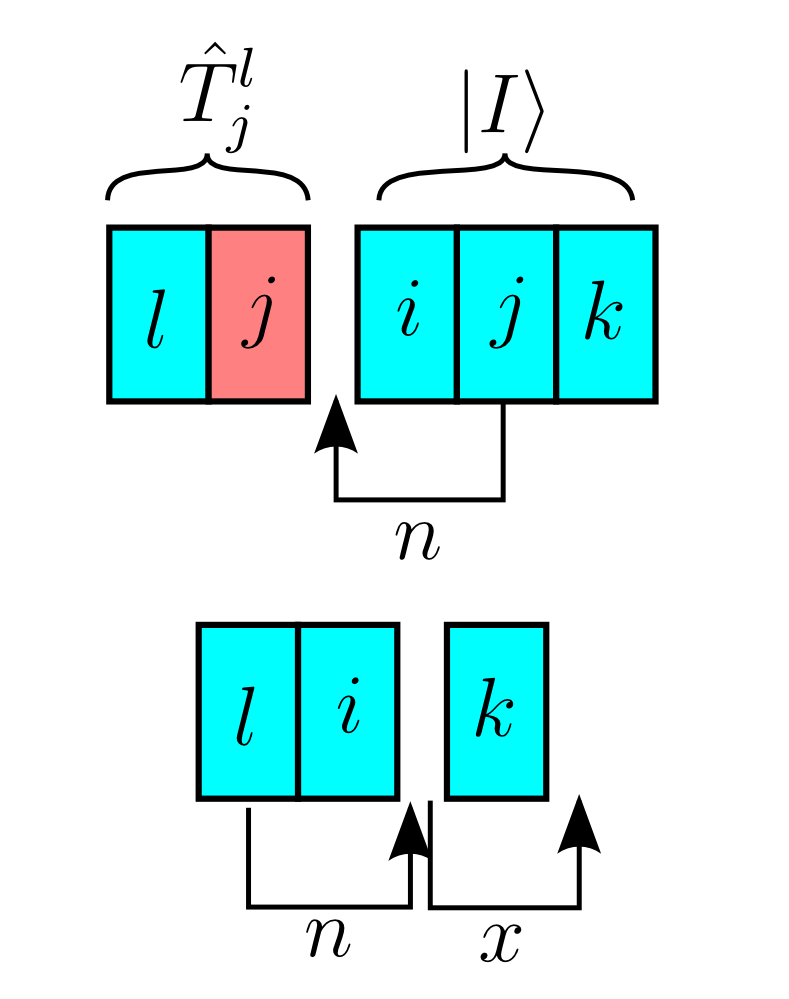
\includegraphics[width=0.3\columnwidth]{figures/determinant_driven/phasefactor}
		\caption{
		\label{phasefactor}%
		phasefactor
		}
	\end{center}
\end{figure}

\subsection{Treating spin parts separately}

It is not immediately obvious that $\alpha$ and $\beta$ spin parts can be treated independently. It is possible because our ordering packs together operators of same spin in the expression of both determinants (Eq.\eqref{eq:spinpack}) and excitations (Eq.\eqref{eq:spinpackexc}), and 
also because we never consider excitations where the spin is changed (spin-flips). 
Under these constraints, any excitation operator $\hat{T}$ can be expressed as 
$$\hat{T} = \hat{T}_\alpha \hat{T}_\beta .$$

\begin{align}
\label{eq:spin1}
\hat{T} \kI & = \hat{T}_\alpha \hat{T}_\beta \,  \hat{I}_\alpha \hat{I}_\beta \vac \\
\label{eq:spin2}
            & =  \qty(\hat{T}_\alpha \hat{I}_\alpha) \qty(\hat{T}_\beta  \hat{I}_\beta) \vac 
              = \hat{J}_\alpha \hat{J}_\beta  \vac = \kJ.
\end{align}

The number of creation and annihilation operators in an excitation operator is always even. Hence, going from Eq.\eqref{eq:spin1} to Eq.\eqref{eq:spin2} by permuting $\hat{T}_\beta$ with $\hat{I}_\alpha$ always requires an even number of permutations.
So the phase factors will be computed by reordering separately $\hat{T}_\alpha \hat{I}_\alpha$ and $\hat{T}_\beta  \hat{I}_\beta$.


%TODO : J'en suis la.


\subsection{Single excitation}

%In the case of a monoexcitation, only one spin part is involved. All indices refer to spinorbitals of same, arbitrary spin $\sigma \in \{\alpha, \beta\}$

For a given determinant $\ket S$ and $\ket{\alpha}=a^\dagger_{j'} a_{i'}  \ket S$, the phase factor of the matrix element $\Hij{S}{\alpha}$ can be determined by the parity of
$$N^{S}_{ij}=\sum_{i<k<j} occ^{S}_{k};i=min(i',j');j=max(i',j')$$
With $occ^{S}_{k}$ the occupation number of spinorbital $k$ for $\ket S$ or $\ket \alpha$. Note that occupation numbers in $\ket S$ and $\ket \alpha$ are by construction equal for any spinorbital $k \neq i \neq j$, so while we will use $\ket S$ in the following, we could as well use $\ket \alpha$. This is obvious from the fact that $\Hij{S}{\alpha}=\Hij{\alpha}{S}$  

Parity of an integer $X$ can be defined by $$p(X)=X \wedge 1$$
        
Indeed $p(X)=0$ if and only if X is even, $p(X)=1$ if and only if X is odd. $p(X)$ is of the same parity as $X$, so 
$$-1^{N_{perm}} = -1^{p(N_{perm})}$$
        
        

A bitstring $R_{ij}$, containing all orbitals in a given range $]i, j>i[$ can be built as follow
$$R_{ij}=ishft(not(0),i) \oplus ishft(not(0),j-1)$$


Be $S$ the bitstring reprensentation of $\ket S$, $N^{S}_{ij}$ The number of $\sigma$ electrons for $\ket S$ in the given orbital range can be evaluated as
$$N^{S}_{ij} = |S_\sigma \wedge R_{ij}|$$

Thus 

$$phase(ij, \ket S) = -1^{p(N^S_{ij})}$$
Using the above formulas and taking into account the bitstring's internal representation as arrays of integer*8 size $\Nint$, we get algorithm \ref{alg:PHASE_MONO}.   


\begin{algorithm}
	\caption{PHASE\_MONO}	
	\label{alg:PHASE_MONO}
				\SetKwFunction{FMain}{PHASE\_MONO}
	\SetKwProg{Fn}{Function}{:}{}
	
	\Fn(\tcc*[h]{Compute phase factor of $\Hij{I}{I_a^b}$}){\FMain{$I_\sigma, a, b$}}{
		\KwData{ $I_\sigma$ the bitstring representation of $\sigma \in \{\alpha, \beta\}$ spinorbitals of $\ket I$}
		\KwData{ $a,b$ indices of a hole and a particle created in $\sigma$ spinorbitals of $\ket I$ }
		\KwResult{ The phase factor associated with $\Hij{I}{I_a^b}$}
		$high \gets max(a,b)-1$ \;
		$low \gets min(a,b)-1$ \;
		$il \gets \frac{low}{64} + 1$ \;
		$ih \gets \frac{high}{64} + 1$ \;
		$l \gets mod(low, 64)$ \;
		$h \gets mod(high, 64)$ \; 
		\For{$i \gets il, ih-1$}{
			$mask[i] = NOT(0)$\;		
		}

		%$mask[ih] \gets ISHFT(NOT(0), h-63)$ \;
		%$mask[il] \gets IAND(mask[il], ISHFT(NOT(0), l))$ \;
		
		$mask[ih] \gets ISHFT(NOT(0), h+1)$ \;
		$mask[il] \gets IEOR(mask[il], ISHFT(NOT(0), l))$ \;
		
		
		$nperm \gets 0$ \;
		\For{$i \gets il,ih$}{
			$nperm \gets nperm + POPCNT(IAND(I_{i}, mask[i]))$ \;
		}
		}
\end{algorithm}
        

\subsection{Phasemasks}


Algorithm \ref{alg:PHASE_MONO} is a general one, efficient for computing the phase factor for two arbitrary determinants. However, a phase computation is typically needed every time an integral is accessed, resulting in a vast amount of computational power being consumed. When only this method was used in the quantum package, it wasn't uncommon to find that most computational power was used on phase computations.
Advantage can be taken of the fact that, in most cases, the considered determinants aren't actually arbitrary. Usually, phase computation will be performed repeatedly on a same determinant, or on determinants of the wavefunction. For a fairly modest computational price, it is possible to compress the phase information from a particular determinant and make it cheaper to extract. The underlying principle is little more than a cumulative sum. If, for a determinant $\ket S$ that is going to be used repeatedely for phase computation, we pre-compute
        
$$E^S_{i} = \sum_{k < i} occ^{S}_{k}$$
        
We can access $N^S_{ij}$ for any $i$ and $j>i$ with no need to loop over $occ^{S}_{k}$

$$\tilde N^S_{ij} = E^S_j - E^S_{i+1} ; i \neq j$$
$$N^S_{ij} = \tilde N^S_{ij} ; j>i$$

Note that $\tilde N^S_{ij}$ is still defined when $j<i$. The reason for this will be made clear later.
This requires to store $E^S$ which is an integer array of size $2 \times (\Norb+1)$. Note that there is a slight waste as $E^S_1 = 0 \forall \ket S$ ( there is always $0$ electrons under the first orbital ) and $E^S_{\Norb+1} = N_{electron,\sigma} \forall \ket S$ ( there is always $N_{electron,\sigma}$ electrons in all orbitals ). Those values are still stored for convenience.






\begin{comment}
This requires to store $E^S$ which is an integer array of size $2 \times (\Norb+1)$.
Note that although only $2 \times \Norb$ integers are required to store the whole information, for practical reasons the actual size of the array is $2 \times (\Norb+1)$ because when the last orbital is involved, we need to access $E_{\Norb+1}$. The reason for this loss is that $E_1$ contains no information - there are always 0 electrons under the first orbital, $E^S_1 = 0 \forall \ket S$.
\end{comment}

This may be somewhat memory consuming if we want to pre-compute and store $E$ for each determinant. However, because the actual information needed isn't $N^S_{ij}$, but merely its parity, we only need to store the so-called "phasemask" vector $P^S$

$$P^S_i = p(E^S_i)$$

which is 1 bit of information per spinorbital, as opposed to an integer big enough to accomodate a number of electrons.
       
$$E^S_i = 2 \times  \lfloor \frac{E^S_i}2 \rfloor + P^S_i$$
$$\tilde N^S_{ij} = E^S_j - E^S_{i+1} = 2 \times \big ( \lfloor \frac{E^S_j}2 \rfloor - \lfloor \frac{E^S_{i+1}}2 \rfloor \big ) + P^S_j - P^S_{i+1}$$
	    
In the last equation, $\tilde N^S_{ij}$ is expressed as a sum of 3 terms. The first one being even by construction, the parity of $\tilde N^S_{ij}$ is the parity of the rest of the sum.
$$p(\tilde N^S_{ij})=p(P^S_j - P^S_{i+1})$$
This can be rewritten in a slightly more efficent way as
$$p(\tilde N^S_{ij}) = P^S_j \oplus P^S_{i+1}$$

Note that using $E^S$ instead of $P^S$ would require an extra ADD instruction ( totalement negligeable ? )
$$p(\tilde N^S_{ij}) = (E^S_{i+1} - E^S_j) \wedge 1$$

We have used sorted indices $i<j$. But just like for the general algorithm, if we consider $\hat T_{i'}^{j'}$, it looks like we need to sort $i'$ and $j'$ to get the $i$ and $j$ indices used for phase computation.

$$i=min(i', j') ; j=max(i', j')$$

This however doesn't need to be done explicitely. We can arbitrarily choose $i=i'$ and $j=j'$, and reverse the phase if $j<i$. We effectively have computed $p(N^S_{i'j'})$ instead of $p(N^S_{j'i'})$, and it can be proven they are always of diffrent parity.

$$\tilde N^{S}_{i' j'} + \tilde N^{S}_{j'i'} = E^{S}_{j'} - E^S_{i'+1} + E^S_{i'} - E^S_{j'+1} = -(occ^S_{j'} + occ^S_{i'})$$

Because $\hat T_{i'}^{j'} \ket S \neq 0$, we know that $occ^S_{j'} + occ^S_{i'} = 1$. 

$$\tilde N^{S}_{j' i'} = -(\tilde N^{S}_{i'j'} + 1)$$

This translates to $\tilde N^{S}_{j' i'}$ and $\tilde N^{S}_{i'j'}$ being of different parity.


\begin{algorithm}
	\caption{PHASEMASK}	
	\label{alg:PHASEMASK}	
	\SetKwFunction{FMain}{PHASEMASK}
	\SetKwProg{Fn}{Function}{:}{}
	
	\Fn(\tcc*[h]{Compute a phasemask}){\FMain{$I$}}{
		\KwData{ $I$ the bitstring representation of $\ket I$}
		\KwResult{ $P$ is the phasemask vector associated with $\ket I$, as described in section XXXXX}
		   
		\For{$\sigma \in \{\alpha, \beta\}$}{
		 $p \gets 0$ \;
		\For{$i \gets 0, \Nint-1$}{
		 $n \gets min(64, \Norb - i \times 64)$ \;
		\For{$j \gets 0,n-1$}{
		 $P_\sigma[i \times 64 + j] \gets p$ \;
		\If{$BTEST(I, j)$}{
		 $p \gets IEOR(p, 1)$ \;
		%\Comment flips the first bit
		}
		}
		}
		 $P_\sigma [\Norb] \gets p$ \;
		}
		\KwRet{$P$} \;
		}
\end{algorithm}


\begin{algorithm}
	\caption{PHASEMASK\_bit}	
	\label{alg:PHASEMASK_bit}	
	\SetKwFunction{FMain}{PHASEMASK\_bit}
	\SetKwProg{Fn}{Function}{:}{}
	
	\Fn(\tcc*[h]{Compute a phasemask}){\FMain{$I$}}{
		\KwData{ $I$ the bitstring representation of $\ket I$}
		\KwResult{ $P$ is the phasemask vector associated with $\ket I$, as described in section XXXXX}
		   
		\For{$\sigma \in \{\alpha, \beta\}$}{
		$r \gets 0$ \;
		\For{$i \gets 0, N_{int}-1$}{
				$P_\sigma[i] \gets \text{IEOR}(I_\sigma[i], \text{ISHFT}(I_\sigma[i], 1)$ \;
				$d \gets 2$ \;
				\While{$d < bit\_kind\_size$}{
					$P_\sigma[i] \gets \text{IEOR}(P_\sigma[i], \text{ISHFT}(P_\sigma[i], d)$ \;
					$d \gets 2 \times d$ \;
				}
				$P_\sigma[i] \gets \text{IEOR}(P_\sigma[i], r)$ \;
				\If{$IAND(\text{POPCNT}(I_\sigma[i]), 1) == 1$}{
					$r \gets \text{NOT}(r)$ \;			
				}
			}
		}
		\KwRet{$P$} \;
		}
\end{algorithm}



\begin{algorithm}
	\caption{PHASE\_FROM\_PHASEMASK}	
	\label{alg:PHASE_FROM_PHASEMASK}	
	\SetKwFunction{FMain}{PHASE\_FROM\_PHASEMASK}
	\SetKwProg{Fn}{Function}{:}{}
	
	\Fn(\tcc*[h]{Compute phase from phasemask}){\FMain{$P^I$, $i$, $j$}}{
		\KwData{ $P^I$ is the phasemask vector associated with $\ket I$, as described in section XXXXX. $i$ and $j$ spinorbitals of spin $\sigma \in \{\alpha, \beta \}$ so that $\hat T_i^j \ket I \neq 0 $}
		\KwResult{ The phase factor of  $\Hij{I}{a_i a^\dagger_j \ket I}$.}

		\uIf{$j < i$}{
			$c \gets 1$ \;
		}
		\Else{
			$c \gets 0$ \;		
		}
		\KwRet{$-1^{(c \oplus P^I_\sigma[i+1] \oplus P^I_\sigma[j])}$} \;
		}
\end{algorithm}

                
\begin{figure}[h!]
	\begin{center}
		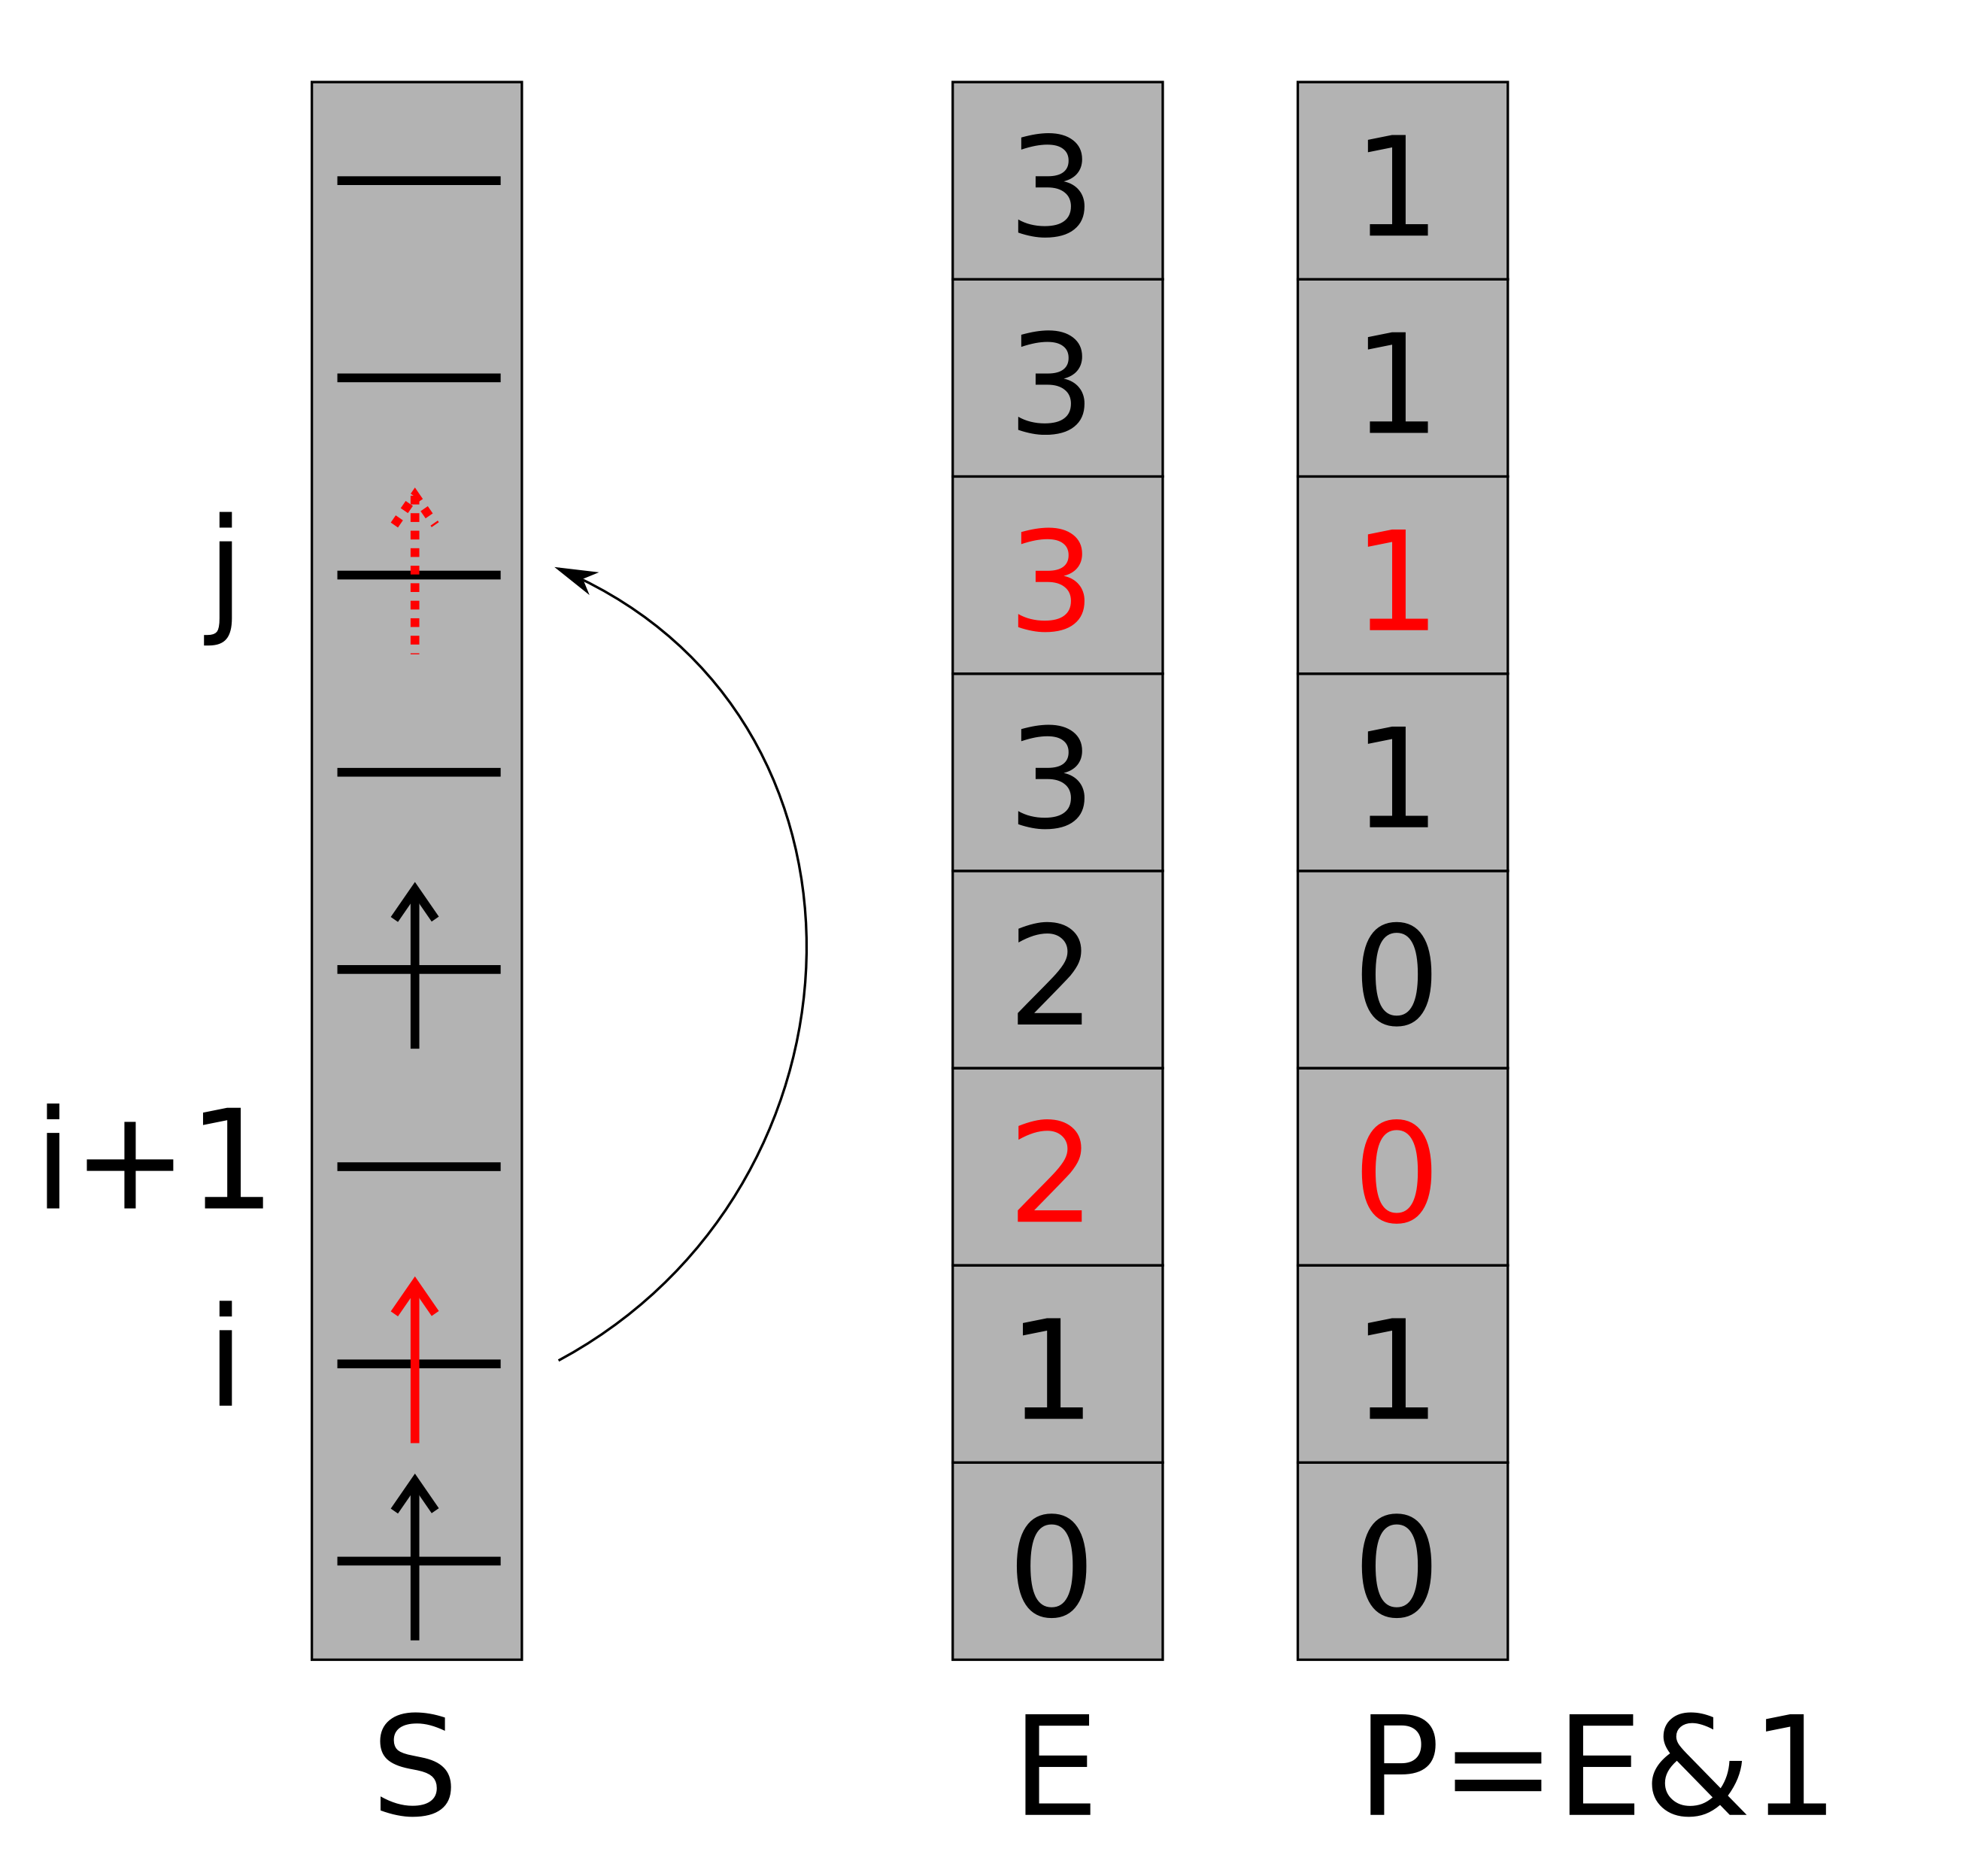
\includegraphics[width=0.6\columnwidth]{figures/determinant_driven/phase}
		\caption{
		\label{generators_selectors}%
		phasemask
		}
		commentt
	\end{center}
\end{figure}
        
Currently, the quantum package does not store the $P$ vector for each variational determinant, but re-computes it whenever needed before a loop. The memory cost being negligible this way, for CPU performance reason, each bit is stored on a separate 32-bit integer.
The algorithm for computing $P^S$ is show as algorithm \ref{alg:PHASEMASK}. 
With this method, the cost of computing a phase - after paying the overhead of computing $P$ - is accessing two integers and IEOR them together (and tests.......). Unlike the general method, its cost doesn't depend on $\Nint$, and doesn't require to deal with the boundaries of 64-bit integers which are ANNOYING AS FUCK.
        

\subsection{Double excitation}







A double excitation is a product of two single excitations.
In the case of an $\alpha \beta$ double excitation, the two single excitations are independant, so the phase factor is merely the product of the phase factors computed for each spin part. 


$$phase(\hat T_{p \bar q}^{r \bar s}, \ket I) = phase(\hat T_{p}^{r}, \ket I) \times phase(\hat T_{ \bar q}^{ \bar s}, \ket I) $$


There is a slight complication for $\alpha \alpha$ or $\beta \beta$ excitations. The ordering we defined for excitation operators is of importance. In order to write a double excitation as a product of two single ones, it must be ensured that the phase (ordering) matches the one we defined : lowest particle with lowest hole, highest particle with highest hole.

As far as phase computation goes, it is irrelevant which index of an exciation operator is a creation and which is an annihilation. So, for convenience, we can write single excitations without defining it

$$\tilde T_{ab} \in \{\hat T_a^b, \hat T_b^a \}$$




Considering a double excitation $\hat T^2$ involving 4 spinorbitals $p,q,r,s$ of same spin, there are two possible situations, shown in figure \ref{fig:biphasefactor}. 



%$$\hat T^2 = \hat T_{pr} \hat T_{qs}$$
%$$\hat T_{pr} \in \{ T_p^r, T_r^p\} ; p<r; \hat T_{qs} \in \{ T_q^s, T_s^q\};q<s$$ 

\begin{itemize}
\item
It can be expressed as two single excitations that do not cross, i.e.
$$\hat T^2=\tilde T_{pr} \tilde T_{qs};p<r<q<s$$
In this case, the numbers of particles in the ranges $]p, r[$ and $]q, s[$ remain unchanged, so we can write
$$phase(\hat T^2, \ket I) = phase(\tilde T_{pr}, \ket I) \times phase(\tilde T_{qs}, \ket I) $$

\item
It can be expressed as two single excitations that cross, i.e.
$$\hat T^2=\tilde T_{pr} \tilde T_{qs};p<q<r<s$$


As we can see in figure \ref{fig:biphasefactor}, applying  $\tilde T_{qs}$ results in a particle being created or annihilated in the range $]p,r[$, resulting in a change of parity for the number of particles in that range. Therefore
$$phase(\tilde T_{pr}, \tilde T_{qs} \ket I) = -phase(\tilde T_{pr}, \ket I)$$ 
$$phase(\hat T^2, \ket I) = -phase(\tilde T_{pr}, \ket I) \times phase(\tilde T_{ qs}, \ket I) $$

\end{itemize}



\begin{figure}[h!]
	\begin{center}
		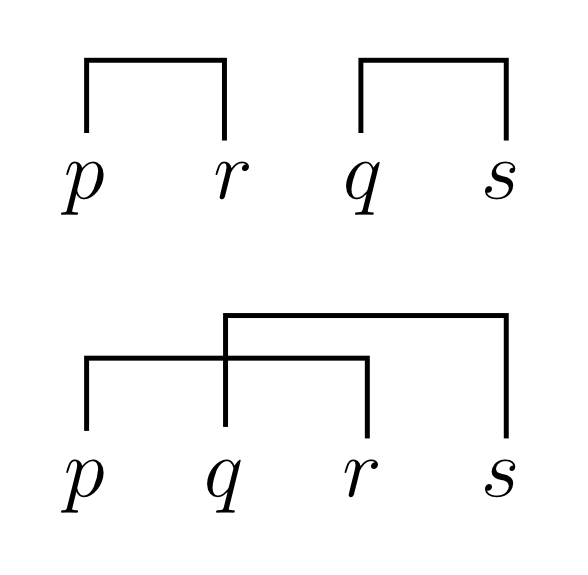
\includegraphics[width=0.4\columnwidth]{figures/determinant_driven/biphasefactor}
		\caption{
		\label{fig:biphasefactor}%
		Crossing of two single excitations
		}
		The third situation doesn't fit the ordering we imposed on excitation operators. $p \leftrightarrow s$ is either lowest electron to highest orbital, or highest electron to lowest orbital.
	\end{center}
\end{figure}

%extra permut si:
%$[(p-r) \oplus (p-s)] \vee [(q-r) \oplus (q-s)] > 0$


\section{integrals}
hashtable \\

\section{generating a subspace}
duplicates are avoided by checking connection to the past \\
******** (ptet exemple avec generator\_CAS versus generator\_full PSI is filtered with different function and supplied to the module using cas\_sd ( cas\_sd, mrcc ) or full\_ci ( pt2 stoch ) )?? \\
================

Generally speaking, a subspace is defined by a reference and a class of excitation applied to it. Because of the determinant-driven approach, it may not be possible to store all the determinants of the considered subspace. 

% - as a matter of fact there is no algorithm to systematically generate all determinants for a defined subspace. The idea to 


\paragraph{reference}

The quantum package allows to define either a CAS or the full-CI as the reference ( although the full-CI is a particular CAS, it is treated differently at the code level ).

\paragraph{excitation class}
The excitations to be applied to the reference are defined by 6 sets of spinorbitals
\begin{itemize}
\item
Holes and particles allowed for single excitations (2 sets)
\item
Holes and particles allowed for the first of a double excitation (2 sets)
\item
Holes and particles allowed for the second of a double excitation (2 sets)
\end{itemize}

This allows to accurately define a subspace. Typically, to define a CAS-SD

\begin{itemize}
\item
\emph{core orbitals} : part of no sets
\item
\emph{inactive orbitals} : part of all "hole" sets
\item
\emph{active orbitals} : part of all sets
\item
\emph{virtual orbitals} : part of all "particle" sets
\item
\emph{deleted orbitals} : part of no set
\end{itemize}


 As will be seen later, determinants are selected iteratively. The general procedure is shown 



\begin{algorithm}
	\caption{GENERAL\_SELECTION}	
	\label{alg:GENERAL_SELECTION}	
	$\ket {\Psi} \gets \ket {HF}$\;
	add CAS spinorbitals to $H_0, H_1, H_2, P_0, P_1, P_2$ \;
	$\hat T$ the list of excitations allowed on the reference based on $H_0, H_1, H_2, P_0, P_1, P_2$ \;
	
	\While{some condition}{
		$C$ the list of determinants of $\Psi$ that are part of the CAS reference \;
		\ForAll{$C_i \in C$}{
			\ForAll{$T_j \in T ; T_j \ket {C_i} \neq 0$}{
				$\ket \alpha \gets T_j \ket {C_i}$ \;
				\If{$not(T_k \ket {C_{l<j}} = \ket \alpha) \&\ Selection\_criterion$}{
					add $\ket \alpha$ to $\Psi '$ \;			
				}
			}
		}
		do some selection in $\Psi'$ \;
		add selected determinants to $\Psi$ \;
		diagonalize $\Psi$ \;
	}
\end{algorithm}

\end{document}


\chapter{Davidson}
\minitoc
\documentclass[./thesis.tex]{subfiles}

 
\begin{document}

Need for variational coefficients. \\
boils down to find connected determinants. \\
Computing excitation is extremely fast already. \\
need to avoid doing comparisons at all \\
Davidson : connections inside a given set \\


\section{def}

\alert{
\begin{itemize}
\item Expliquer que la diagonalisation est en $\order{N^3}$, et donc pas viable pour des millions de determinants. On n'est interesse que par les plus basses valeurs propres de $H$, donc on peut utiliser une methode iterative pour les obtenir.
\item Raconter ce qu'il y a dans le papier original : [ E.R.  Davidson, J.  Comput.  Phys.  17 (1975) 87 ].
\item Mettre le pseudocode de l'algorithme.
\item Parler de quelques ameliorations depuis : [ J.  Olsen, P.  Joregensen and J.  Simons, Chem.  Phys.  Letters 169 (1990) 463 ], [F.X.  Gadea /Chemical Physics Letters 227 (1994) 201-210] 
\item Dire qu'on utilise l'algorithme original parce qu'on a toujours un bon guess (CIPSI)
\item Pour etre fonction propre de $S^2$ on utilise une penalty method, comme dans [10.1021/acs.jctc.7b00466]. (D'ailleurs dans ce papier il y a un pseudocode pour Davidson). Et tu peux ajouter qu'on calcule $S^2c$ en meme temps que $Hc$.
\end{itemize}
}

    
\section{general approach}
Algorithmically, the expensive part of the Davidson diagonalization is the computation of the matrix-vector products $\mH \mc$.

Determinants are connected by $\mH$ only if they differ by no more than two spinorbitals. Therefore, the number of non-zero elements per line of $\mH$ is equal to the number of single and double excitation operators, namely $\order{\Nelec^2 \times (\Norb - \Nelec)^2}$. As $\mH$ is symmetric, the number of non-zero elements per column is identical. This makes the $\mH$ matrix very sparse, but for large basis sets the whole $\mH$ matrix may not fit in the memory of a single node, as the number of non-zero entries to store is $\order{\Ndet \times \Nelec^2 \times (\Norb - \Nelec)^2}$. 
One possibility would be to distribute the storage of Hamiltonian among multiple compute nodes, and use a distributed library such as PBLAS\cite{pblas} to perform the matrix-vector operations. Another approach is to use a so-called \emph{direct} algorithm, where the matrix elements are computed \emph{on the fly}, and this is the approach chosen in the \QP.


This effectively means iterating over all pairs of determinants $\ki$ and $\kj$, checking whether $\ki$ and $\kj$ are connected by $\mH$ and if they are, accessing the corresponding integral(s) and computing the phase factor.
Even though we presented a very effective method to compute the excitation degree between two determinants, the number of such computations to be made scales as $\Ndet^2$, which can be prohibitively high. To get an efficient implementation it is mandatory to filter out all pairs of determinants that are not connected by $\mH$.
The base approach to this problem is to sort, or rather classify, determinants so as to build sets that are by construction disconnected from others. Generally speaking, the set of all determinants is split in disjoint sets $S_c$, $c$ being a mathematical object of the set $\mathcal{T}$. $\mathcal{D}$ is the set of determinants. For a specific method, we have the functions
\begin{itemize}
	\item
	$C : \mathcal{D} \rightarrow \mathcal{T}$, a function that takes a determinant and returns a value in $\mathcal{T}$
	\item
	$p : \mathcal{T}^2 \rightarrow \{ \TRUE, \FALSE \}$, a function that takes a pair $(x,y) \in \mathcal{T}^2$, and returns $\FALSE$ if all the determinants of $S_x$ are disconnected to all the determinants of $S_y$, $\TRUE$ otherwise.
	\item
	$D \in S_{C(D)}$
\end{itemize}  

%TODO : J'en suis la 

Although it's not formally needed, it is pretty much necessary in practice to have some comparison operator for elements of $\mathcal{T}$, so that sets can be easily formed by sorting determinants according to their respective $C(D)$. However, the choice for this operator is entirely arbitrary and doesn't affect the method, so it will not be discussed.
    
    
We can then represent the cost of computing $\mH$ using a matrix $\mathbf{M}$ of same size, where each element $M_{ij}=1$ if the corresponding element $H_{ij}$ needs to be computed, and $M_{ij}=0$ if it is known to be zero by construction.

\alert{
Theoretical representation of $\mathbf{M}$ with 3 classes of determinants $A$, $B$, and $C$, $A$ and $C$ being by construction disconnected. $H_{ij}$ elements corresponding to the white area are, by construction, known to be null. Those in the yellow area need to be computed.
}
    
\begin{figure}[h!]
	\begin{center}
		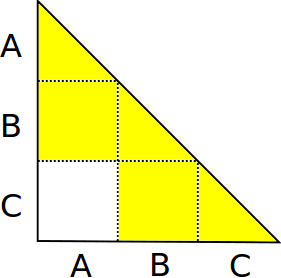
\includegraphics[width=0.4\columnwidth]{figures/davidson/disconnected_classes}
		\caption{{\label{generators_selectors}
		}}
	\end{center}
\end{figure}

Because the number of determinants used in the following examples is 500k, $M$ is shown as a density map.

As an example, one of the first attempted classification was according to the number of electrons in $s$ a subset of orbitals. Indeed, if $\ket I$ has $n$ electrons in an arbitrary subset of orbitals, and $\ket J$ has $n-3$, quite obviously it will take at least 3 excitations to excite from $\ket I$ to $\ket J$.
\begin{itemize}
	\item
	$\mathcal{T}$ is type scalar
	\item
	$C(D)$ returns the number of electrons in the chosen subset.
	\item
	$p(x, y) = |x-y| \leq 2$
\end{itemize}

Computation of $C(D)$ can be acheived using bitstrings. With $S$ a bitstring containing the orbitals wanted in the subset. The number of electrons in this subset for a determinant $\ket I$ represented by a $\alpha \beta$-bitstring $I$ is
\begin{equation}
C(I)=|I_{\alpha} \wedge S|+|I_{\beta} \wedge S|
\end{equation}

Using a subset is equivalent to using the complementary subset, so it is best to pick $N_{orb}/2$ orbitals. For a better entropy, it is of course better to interleave the chosen orbitals.
\begin{equation}
S=binary(...101010101...)
\end{equation}
    
Determinants are sorted according to this criterion. Using ClBr with 500k determinants, and sorting determinant in increasing order of their respecive $C(D)$, we got matrix $M$ shown in figure \ref{fig:num_subspace}

\begin{figure}[h!]
	\begin{center}
		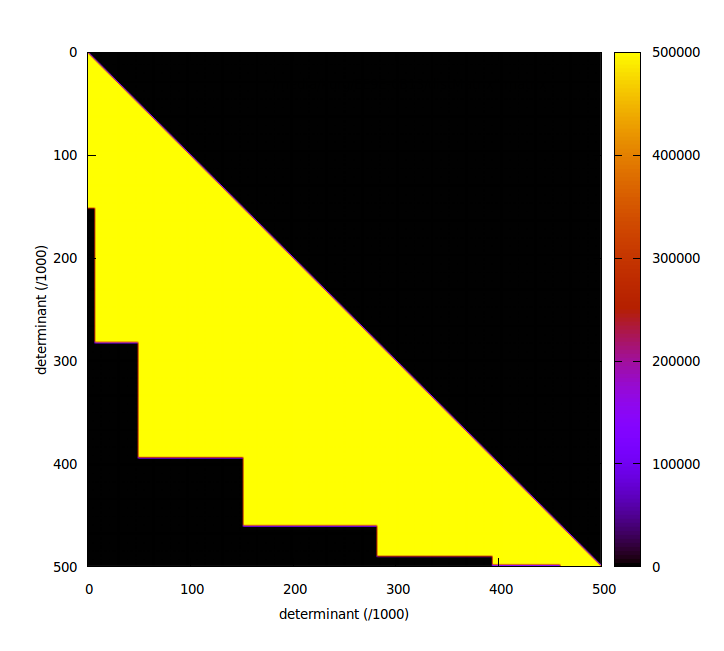
\includegraphics[width=0.6\columnwidth]{figures/davidson/num_subspace}
		\caption{{\label{fig:num_subspace}
		}}
	\end{center}
\end{figure}
    
As expected, the farther away two determinants $\ket I$ and $\ket J$ are in the sorted determinant vector, the likelier it is that $|C(I)-C(J)| > 2$ which makes them disconnected by construction. The "staircase" aspect shows the boundaries of each class.
However, only a relatively small area of $H$ is null by construction. It is possible to further reduce the area to be explored by chosing several orbital subsets $S_1$ to $S_n$ instead of a single one. In this case, $C(D)$ returns $c$ a vector of size $n$ with $c_{i}$ the number of electron in subset $S_i$ for $D$

\begin{itemize}
	\item
	$\mathcal{T}$ is type vector size $n$
	\item
	$C(D)$ returns $c$ a vector of size $n$, $c_i$ the number of electron in subset $S_i$
	\item
	$p(x, y) = |x_i - y_i| \leq 2 \forall i$
\end{itemize}



Using $n=3$ uncorrelated subsets
\begin{equation}
S_1 = binary(...010101010101...)
\end{equation}
\begin{equation}
S_2 = binary(...110011001100...)
\end{equation}
\begin{equation}
S_3 = binary(...111100001111...)
\end{equation}
The resulting $M$ in figure \ref{fig:num_subspace3} looks awesome but the area isn't reduced much.

\begin{figure}[h!]
	\begin{center}
		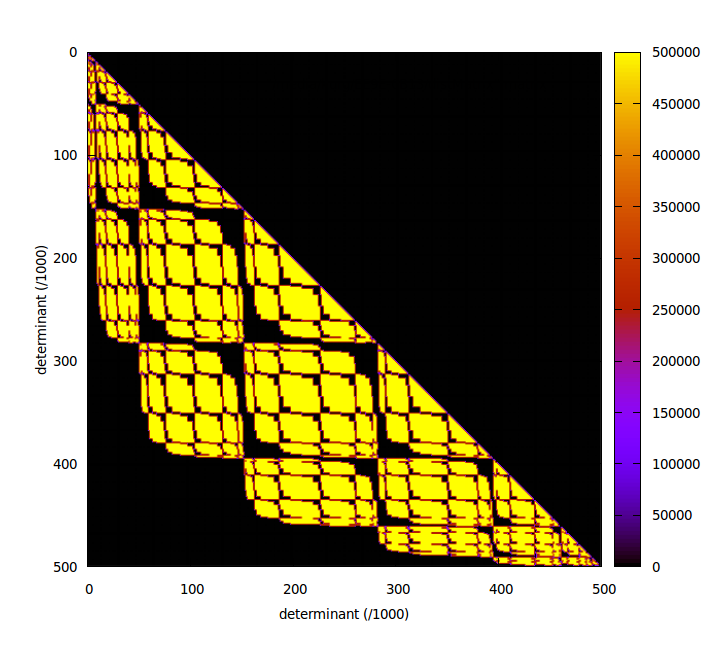
\includegraphics[width=0.6\columnwidth]{figures/davidson/num_subspace3}
		\caption{{\label{fig:num_subspace3}
		}}
	\end{center}
\end{figure}


\section{A few methods of interest}

A few methods happened to be of interest
\subsection{Highest electrons}
This method hasn't been explored throughoutly, but is still mentioned as it showed potentially interesting results, and can be use in combination with other methods.
The highest electrons are the most mobile ones, so they are the most likely not to match between two determinants. 

\begin{itemize}
	\item
$n \geq 3$ is a parameter of the method. 
	\item
$\mathcal{T}$ is a set of $n \geq 3$ electrons. 
	\item
$C(D)$ returns the set of the $n$ highest occupied spinorbitals of $D$. To make this unambiguous, it is arbitrarily decided that $\alpha$ spinorbitals are considered higher than their $\beta$ counterpart of same index.
	\item
$p(x, y) = n - |x \wedge y)| \leq 2$
\end{itemize}

$n$ is typically 3 or 4, as a greater value will result in lots of singletons, and the whole point of grouping determinants into sets being defeated. In the extreme case where $n = N_{electron}$, $C(D) = D$
   


\subsection{Singly occupied orbitals}
If there are $n$ orbitals that are singly occupied in $\ket I$ and not singly occupied in $\ket J$, it will take at least $n$ excitations to excite between $\ket I$ and $\ket J$.

\begin{itemize}
	\item
$\mathcal{T}$ is a set of orbitals
	\item
$C(D)$ returns the set of singly occupied orbitals in $D$
	\item
%$p(x, y) = max \big [popcnt(iand(x, z)), popcnt(iand(y, z)) \big ] > 2 ; z = ieor(x, y)$
$p(x, y) = max (|x|, |y|) - |x \wedge y| \leq 2$
\end{itemize}

Matrix $M$ for that method is shown in figure \ref{fig:xor_subspace}.
This method has one interesting property. If we compare determinants only with those contained in the same set - which is a tiny fraction of the total number of comparisons to be performed - we are guaranteed to find all excitations of the form $\hat T_{a \bar a}^{b \bar b}$ and $\hat T_{a \bar b}^{b \bar a}$, which are typically the largest non-diagonal matrix elements. Indeed, those excitations imply there was no change in singly occupied orbitals. And since they are the only one to do so, we are also guaranteed not to find any other type of excitation within a set.

\begin{figure}[H]
	\begin{center}
		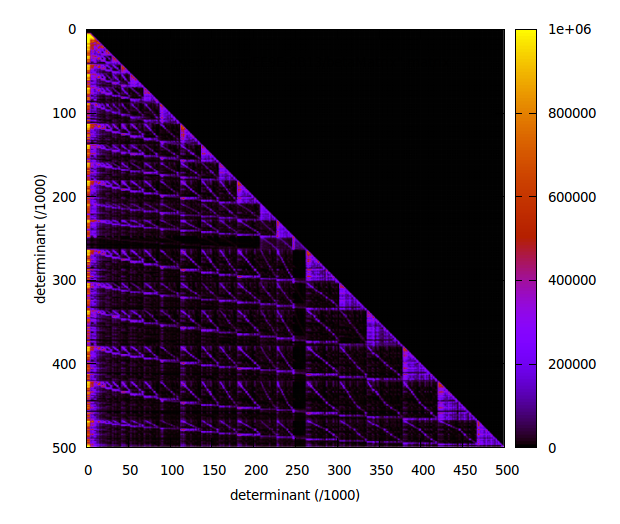
\includegraphics[width=0.6\columnwidth]{figures/davidson/xor_subspace}
		\caption{{\label{fig:xor_subspace}
		}}
	\end{center}
\end{figure}


\subsection{Simple spin part}
This methods has been implemented but was overriden by Composite spin part, introduced next. It is mostly mentioned for comprehension.

\begin{itemize}
	\item
$\mathcal{T}$ is a set of $\alpha$ spinorbitals
	\item
$C(D)$ returns $D_\alpha$, the set of occupied $\alpha$ spinorbitals in $D$
	\item
$p(x, y) = \frac{|x \oplus y|}{2} \leq 2$
\end{itemize}

$\frac{|x \oplus y|}{2}$ computes the excitation degree between $x$ and $y$ spin parts. 
    

    
\subsection{Composite spin part}
What can be noticed in the previous method, is that when we compute $p(x, y)$ to check if two sets $S_x$ and $S_y$ are disconnected, the value returned is the excitation degree for the $\alpha$ part between any $D_1 \in S_x$ and $D_2 \in S_y$. If $p(x, y)=2$, it means, $D_1$ and $D_2$ can only be connected if the excitation for the $\beta$ part is 0, in other words, if they share the same $\beta$ part. This in turn means that, when we compare determinants from $S_x$ and $S_y$, we are only looking for determinants with equal $\beta$ spin part.
Had we chosen $C(D)$ to return the $\beta$ spin part instead of the $\alpha$ one, $D_1$ and $D_2$ would have ended in the same set.
Taking this into account, we can set up a method that is made of two sub-methods, each one finding of a subset of possible excitations.

\begin{itemize}
\item
Find all connections between determinants that share the same $\alpha$ spin part. In other words, it finds all purely $\beta$ excitation,$\hat T_{\bar a}^{\bar b}$ and $\hat T_{\bar a \bar b}^{\bar c \bar d}$
\begin{itemize}
	\item
$\mathcal{T}_\alpha$ is a set of $\alpha$ spinorbitals
	\item
$C_\alpha(D)$ is the set of occupied $\alpha$ spinorbitals in $D$
	\item
%$p_\alpha(x, y) = max \big [popcnt(iand(x, z)), popcnt(iand(y, z)) \big ] > 2$, with $z = ieor(x, y)$
$p_\alpha(x, y) = (x = y)$
\end{itemize}
\item
Find all connections between determinants that are at most singly excited in their $\beta$ part.
This includes purely $\alpha$ excitation as well as $\alpha+\beta$ ones, $\hat T_a^b$, $\hat T_{ab}^{cd}$ and $\hat T_{\bar a b}^{\bar c d}$.
\begin{itemize}
	\item
$\mathcal{T}_\beta$ is a set of $\beta$ spinorbitals
	\item
$C_\beta(D)$ is the set of occupied $\beta$ spinorbitals in $D$
	\item
$p_\beta(x, y) = \frac{|x \oplus y|}{2} \leq 1$
\end{itemize}
\end{itemize}
    

All types of double excitations are found by either sub-method. The resulting $M$ matrices are shown in figures \ref{fig:aabb_subspace} and \ref{fig:ab_subspace}.
The point of this method compared to the previous one, is that the $p$ condition is drastically tightened, resulting in many more sets being by construction disconnected. For the simple spin part method, given a spin part $x$, the cardinality of the set of all $y$ spin parts so that $p(x, y) = TRUE$ is the number of possible double excitations. For composite spin part, it is respectively 1 ($p_\alpha$) and the number of single excitations ($p_\beta$).
As can be seen, the first method, although it finds all purely $\beta$ excitations, and could as well be used to find purely $\alpha$ ones, explores a minuscule area of $H$. As a matter of fact, finding those is pretty much "free", the vast majority of computational time is spent finding $\alpha \beta$ excitations.
As previously seen, the most important of excitations, those of the form $\hat T_{a \bar b}^{b \bar a}$, happen to be $\alpha \beta$ ones and can also be obtained for a very small cost using the singly occupied orbitals method. ( et donc? )

    
    \begin{figure}[H]
	\begin{center}
		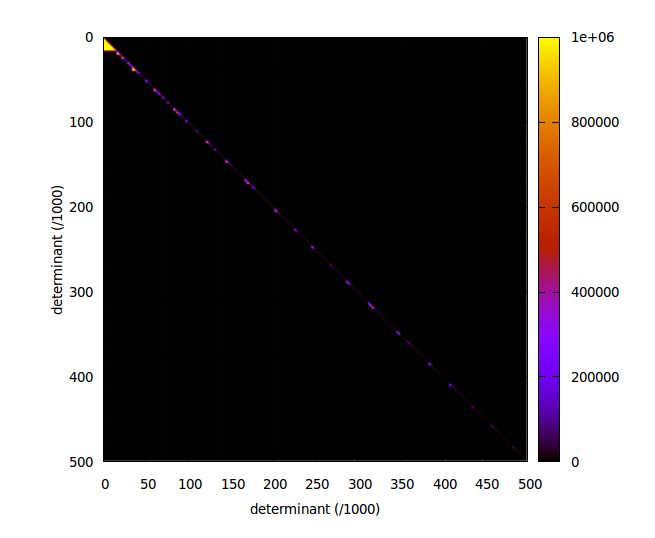
\includegraphics[width=0.6\columnwidth]{figures/davidson/aabb_subspace}
		\caption{{\label{fig:aabb_subspace}
		}}
	\end{center}
\end{figure}

\begin{figure}[H]
	\begin{center}
		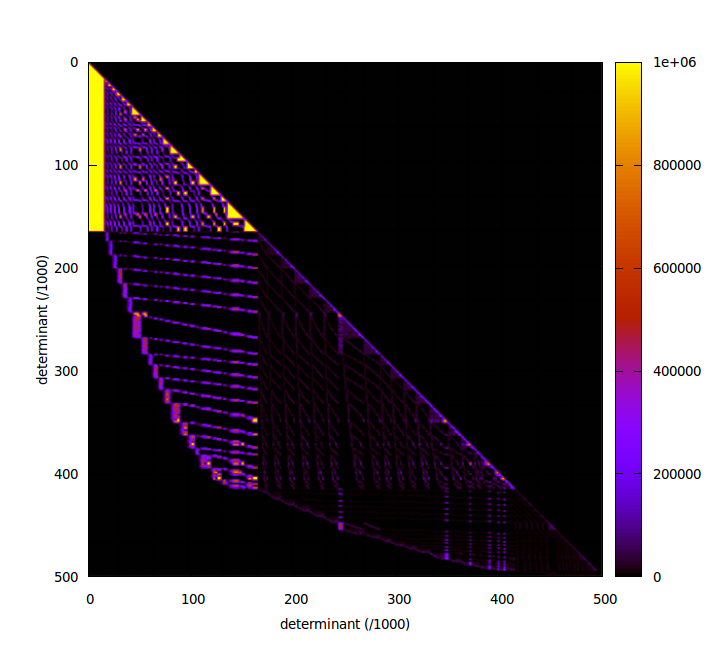
\includegraphics[width=0.55\columnwidth]{figures/davidson/ab_subspace}
		\caption{{\label{fig:ab_subspace}
		}}
	\end{center}
\end{figure}

\section{excitation driven(?) - (TOTO, INUTILE DE LIRE) a reecrire/tester}

There is a way to find connections using an 'excitation driven' approach, that would be closer to an integral-driven approach. Essentially, it is possible to find all determinants of an arbitrary set that connects by a particular excitation, with a complexity linear (logarithmic???) with $N_{det}$.
To understand this approach, we will considered bitstrings as single integers of arbitrary size.

SCHEMA


\begin{equation}
\hat T_{a}^{b} D = E
\end{equation}

\begin{equation}
ibclr(ibset(I_D, b), a)
\end{equation}
 
 
\begin{equation}
ibclr(X, a) = X - ISHFT(1,a) ; ibtest(X,a) == TRUE
\end{equation}

\begin{equation}
ibset(X, b) = X + ISHFT(1,b) ; ibtest(X,b) == FALSE
\end{equation}

If $\hat T_{a}^b$ can be applied to $D$, 
\begin{equation}
ibtest(I_D,a)\ and\ not\ ibtest(I_D,b)
\end{equation}

\begin{equation}
I_E = I_D + I_T ; I_T = ISHFT(1,b) - ISHFT(1,a)
\end{equation}

As can be seen, it is possible to have an integer representation of an excitation.

\begin{equation}
TD = E \implies I_E = I_D + I_T ; E \neq 0
\end{equation}

It must be noted that, if $T$ cannot be applied to $D$, $I_E = I_D + I_T$ will, in most cases, not be a valid reprensentation of a determinant ; that is, $popcnt(I_{E_\alpha}) \neq N_{e,\alpha} \vee popcnt(I_{E_\beta}) \neq N_{e,\beta}$. However, there are rare instances where this isn't true.

EXEMPLE avec 8bit?

Therefore, if $I_E - I_D = I_T$, additional checks are required to establish that $TD = E$.


Implementing this in Fortran may not looks straightforward considering in this language, integers are always signed, thus the leftmost bit has a special status. However, it is actually of no relevance except when it comes to sorting, and merely changing the sorting order won't cause any malfunction.
If "signed" sorting is however desired, it can easily be emulated. Be $X$ and $Y$ two 64-bit integers, $u_comp$ the unsigned comparison operator (the one used by Fortran) and $s_comp$ the signed comparison operator.

\begin{equation}
s\_comp(X,Y) = u\_comp(IEOR(X,ISHFT(1,63)), IEOR(Y,ISHFT(1,63))
\end{equation}


$IEOR(X,ISHFT(1,63)$ returns $X$ with bit at position 63 flipped. Bit are indexed from 0 so bit at position 63 is the leftmost one for 64-bit integers.

The algorithm for "excitation driven" connection finding is detailed in algorithm XX.

=========


\begin{comment}




\begin{algorithm}
	\caption{base functions}
		
	\SetKwFunction{FMain}{AddBigint}
	\SetKwProg{Fn}{Function}{:}{}
	
	\Fn(\tcc*[h]{co}){\FMain{some args}}{
		$overflow \gets 0$ \;
		\For{$i=1,N_{int}$}{
			$may \gets IOR(I[i], J[i])$ \;
			$will \gets IAND(I[i], J[i])$ \;
			$R[i] = I[i] + J[i] + overflow$ \;
			$overflow = ISHFT(IOR(will, IAND(may, not(R[i]))), -63)$ \;
		}
	}
\end{algorithm}


\begin{algorithm}
	\caption{base functions}
		
	\SetKwFunction{FMain}{AddBigint}
	\SetKwProg{Fn}{Function}{:}{}
	
	\Fn(\tcc*[h]{co}){\FMain{some args}}{
		$i \gets 1$ \;
		$j \gets 1$ \;
		\While{$i \leq N_i \& j \leq N_j$}{
			\For{$\sigma = \{\alpha, \beta\}$}{
			$overflow \gets 0$ \;
			\For{$k=1,N_{int}$}{
				$m \gets I_i[k,\sigma] + E[k, \sigma] + overflow$ \;
				\uIf{$m > J_j[k, \sigma]$}{
					$j \gets j+1$ \;
					cycle i,j loop \;
				}\ElseIf{$m < J_j[k, \sigma]$}{
					$i \gets i+1$ \;
					cycle i,j loop \;
				}
				$may \gets IOR(I_i[k,\sigma], E[k, \sigma])$ \;
				$will \gets IAND(I_i[k,\sigma], E[k, \sigma])$ \;
				$overflow \gets ISHFT(IOR(will, IAND(may, not(m))), -63)$ \;
			}
			}
			\If{$EXC(I_i, J_j) \leq 2$}{
				$assert(J=EI)$ \;			
			}
		}
	}
\end{algorithm}





\begin{algorithm}
	\caption{base functions}
	\label{EXCITATION_DRIVEN}
	\SetKwFunction{FMain}{EXCITATION\_DRIVEN}
	\SetKwProg{Fn}{Function}{:}{}
	
		\Fn(\tcc*[h]{A VERIFIER}){\FMain{some args}}{
		$i \gets 1$ \;
		$j \gets 1$ \;
		

		\While{$i \leq N_i \& j \leq N_j$}{
			$aim \gets APPLY(I_i, E, ok)$ \;
			\If{$not\ ok$}{
				$i \gets i+1$ \;
				cycle \;
			}
			\While{$j \leq N_j$}{
				\tcc{find the index of $aim$ in $J$ in the range $[j, N_j]$. If not found, return the lowest $j$ so that $detCmp(aim, J_j) = 1$, or $N_{j}+1$ if $aim > J_{N_j}$.}
				$j \gets find(aim, J, j, N_j, ok)$ \;
				\If{$ok$}{
					found \;
				}
				%				$cmp \gets DetCmp(J_j, aim)$ \;
%				\uIf{$cmp = 1$}{
%					break \;
%				}\ElseIf{$cmp = 0$}{
%					found \;
%					break \;
%				}
%				$j \gets j+1$ \;
			}
		}

	}
	
			
	\SetKwFunction{FDetCmp}{DetCmp}
	\SetKwProg{Fn}{Function}{:}{}
	
	\Fn(\tcc*[h]{co}){\FDetCmp{$I$, $J$}}{
		\For{$\sigma = \{\alpha, \beta\}$}{
		\For{$k=1,N_{int}$}{
			\uIf{$I_\sigma[k] > J_\sigma[k]$}{
				\KwRet{1} \;
			}\uElseIf{$I_\sigma[k] < J_\sigma[k]$}{
				\KwRet{-1} \;
			}
		}
		}
		\KwRet 0 \;
	}
\end{algorithm}
\end{comment}



\begin{algorithm}
	\caption{EXCITATION\_DRIVEN}
	\label{EXCITATION_DRIVEN}
	\SetKwFunction{FMain}{EXCITATION\_DRIVEN}
	\SetKwProg{Fn}{Function}{:}{}
	
		\Fn(\tcc*[h]{CHECK}){\FMain{$I$, $J$}}{
		$i \gets 1$ \;
		$j \gets 1$ \;
		

		\While{$i \leq N_I \& j \leq N_J$}{
			$aim \gets APPLY(I_i, E, ok)$ \;
			$j \gets find\_first\_geq(aim, J, j, N_j, match)$ \;				
			
			\If{$not(match) \& j \leq N_j$}{
				$aim \gets REVERSE\_APPLY(J_j, E, ok)$ \;
				$i \gets find\_first\_geq(aim, I, i, N_i, match)$ \;
				
			}
			\If{$match$}{
				\If{$ok$}{
					assert $J_j = \hat EI_i$ \;	
				}
				$i \gets i+1$ \;
			}
		}
	}

	
	
			
	\SetKwFunction{FDetCmp}{DetCmp}
	\SetKwProg{Fn}{Function}{:}{}
	
	\Fn(\tcc*[h]{REPLACE WITH find\_first\_geq}){\FDetCmp{$I$, $J$}}{
		\For{$\sigma = \{\alpha, \beta\}$}{
		\For{$k=1,N_{int}$}{
			\uIf{$I_\sigma[k] > J_\sigma[k]$}{
				\KwRet{1} \;
			}\uElseIf{$I_\sigma[k] < J_\sigma[k]$}{
				\KwRet{-1} \;
			}
		}
		}
		\KwRet 0 \;
	}
\end{algorithm}


Final idea : alpha/beta with integrals in hashtable \\
%Next idea(?) : singly occupied with T|I> = T+I \\
parallelisation  ************* \\

\end{document}


\chapter{CIPSI}
\minitoc
\documentclass[./thesis.tex]{subfiles}


\begin{document}
\label{chap:CIPSI}


\section{The basic algorithm}
My initial and most important work has been the improvement of the implementation of the CIPSI algorithm present in the \QP, that had been implemented by my predecessor.\cite{giner:tel-01077016} As was briefly described in section~\ref{sec:meth_cipsi}, it is an \emph{on the fly} iterative selection algorithm, where determinants are added to the variational wavefunction according to a perturbative criterion. Because it gathers a large amount of information, this CIPSI implementation has been the basis for other subsequent works presented in the next chapters.

The $n^\text{th}$ iteration of CIPSI can be described like so:

\begin{enumerate}
\item

The variational function $\ket {\Psi^{(n)}}$ is defined over a set of determinants $\{\ket{D_I}\}^{(n)}$ in which we diagonalize $\widehat{H}$
\begin{equation}
\ket{\Psi^{(n)}} = \sum_{I} c_I^{(n)} \kI
\end{equation}
The determinants in $\{\ket{D_I}\}^{(n)}$ will be characterized as \emph{internal}.

\item
For all \emph{external} determinants $\kalpha \notin \{\ket{D_I}\}^{(n)}$, we compute the perturbative contribution
\begin{equation}
e_\alpha = \frac{\Hij{\Psi^{(n)}}{\alpha}^2}{E^{(n)} - \Hij{\alpha}{\alpha}}.
\end{equation}
As we use Epstein-Nesbet perturbation theory, $E^{(n)}=\Evar^{(n)}$ is the variational energy of the wavefunction at the current iteration (note that another perturbation theory could be used here).

\item Summing the contributions of all the external determinants gives the second order perturbative correction
\begin{equation}
\EPT^{(n)} = \sum_{\alpha} e_\alpha
\end{equation}
and the FCI energy $\EFCI$ can be estimated
\begin{equation}
\EFCI \approx \Evar^{(n)} + \EPT^{(n)}
\end{equation}

\item
We extract $\{ \ket{\alpha_\star} \}^{(n)}$ the subset of determinants $\kalpha$ with the largest contributions $e_\alpha$, and add them to the variational space
\begin{equation}
\{\ket{D_I}\}^{(n+1)} = \{\ket{D_I}\}^{(n)} \cup \{ \ket {\alpha_\star} \}^{(n)}
\end{equation}

\item
Go to iteration $n+1$, or exit on some criterion (number of determinants in the wavefunction, low $\EPT^{(n)}$, \dots).

\end{enumerate}



As can be seen, CIPSI involves the creation of an external space and a precise knowledge of how it interacts with the internal space. Algorithmically speaking, we will need to enumerate all connections between all internal and all external determinants.
There are, perhaps schematically, two ways to do this :

\begin{itemize}
\item
``external to internal'', looping over all possible $\kalpha$ and computing $e_\alpha$.
\item
``internal to external'', looping over all internal determinants $\kI$ and all single or double excitations $\hat T$, creating $\kalpha = \delta \qty(\braket{\Psi}{\alpha} ) \ordering \hat T \kI$, then incrementing $\tilde e_{\alpha}$ by $c_I\Hij{D_I}{\alpha}$. Finally get $e_{\alpha} = \frac{\tilde e_\alpha^2}{E^{(n)} - H_{\alpha \alpha}}$.
\end{itemize}

%\begin{figure}[h!]
	\begin{center}
		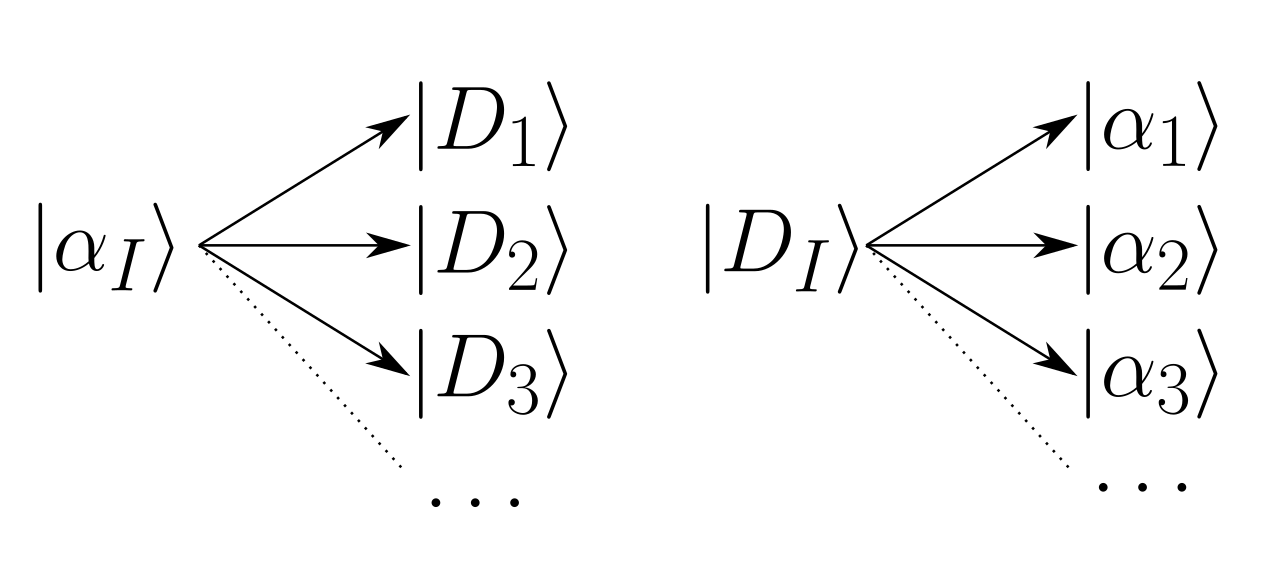
\includegraphics[width=0.45\columnwidth]{figures/matrix_dressing/interactions}
	\end{center}
	%\caption{\label{interactions}}
%\end{figure}

The first approach is less tempting, as it means finding connections between the arbitrary set of internal determinants, and another arbitrary set of $\kalpha$ typically orders of magnitude larger.

While the second approach sounds more straightforward, it has the obvious issue of requiring all $e_\alpha$ to be stored in memory simultaneously. Unfortunately this is usually not feasible, since their number scales as $\order{\Ndet \times \Nalpha^2 \times \qty(\Norb - \Nalpha)^2}$.
The first approach therefore seems simpler when it comes to computing $e_\alpha$, but it begs the question of how to generate all possible $\kalpha$ with no duplicates. 

Both our former and newer implementations of CIPSI generate the external space in an ``internal to external'' way, that is, by applying single and double excitations to internal determinants ; a determinant used to generate $\kalpha$ is referred to as a \emph{generator}.
Ensuring each $e_\alpha$ is considered only once is done by checking that all the determinants $\kalpha$ generated by the generator $\kI$ are not connected to any of the generators in $\{ \ket{D_{J<I}} \}$.
If a connection $\hat T$ is found, it means that $\kalpha$ is generated from $\kJ$ as $\ordering \hat T \kJ$, and should not be considered by the current generator.

\section{Approximations}
\label{sec:cipsi_approx}

Given the qualitative nature of this procedure ---~each $\kalpha$ is either selected or not~--- it is possible to save a vast amount of computational time with minimal approximations. These were present in the original implementation and retained in the new one.

From now on, we will consider that the determinants are sorted such that 
\begin{equation}
c^2_{I} \ge c_{I+1}^2
\end{equation}

Two approximations are made :

\begin{itemize}
\item
The first approximation restricts the set $\{\kalpha\}$. It is very unlikely $\ket \alpha$ will be selected if it is not connected to any $\kI$ with a large coefficient. Therefore, it is possible to only consider the determinants of larger coefficient as generators. We choose a number of generators $\Ngen$ and only consider $\ket{D_{I \leq \Ngen}}$ as generators. In practice we set $\Ngen$ according to a norm threshold $n_g$, picking $\Ngen$ as the highest value fulfilling
\begin{equation}
\sum_{I \leq \Ngen} c_I^2 \leq n_g.
\end{equation}
This approximation is a variant of the \emph{three-class CIPSI},\cite{Evangelisti_1983}
and typically $n_g=0.99$ is used in the calculations.
\item The second approximation reduces the cost of $e_\alpha$.
We do not need extremely accurate values for $e_\alpha$ as small differences are unlikely to substantially change the subset of the largest ones.
So  connections to $\ket {D_I}$ with small coefficients $|c_I|$ can be neglected
in the expression of $e_\alpha$.
This approximation is achieved in a similar way by defining a threshold $n_s$
on the norm of the wavefunction, and $N_{sel} \geq \Ngen$ a number of so-called
\emph{selectors}. We approximate 
\begin{equation}
  \Hij{\Psi}{\alpha} \approx \sum_{I \leq N_{sel}} c_I \Hij{D_I}{\alpha}.
\end{equation}
Typically, we use $n_s = 0.999$.

\end{itemize}

Note that generator determinants are a subset of selector determinants. See figure \ref{fig:generators_selectors}.


\begin{figure}[h!]
        
        \begin{center}
                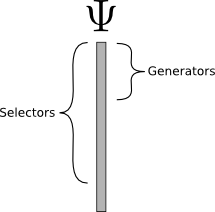
\includegraphics[width=0.25\columnwidth]{figures/cipsi/selexemple2}
        \end{center}
        \caption{Determinants are sorted by decreasing $c_I^2$ ; generator and selector subsets are defined.}
        \label{fig:generators_selectors}
\end{figure}



\section{Initial implementation}

Originally, the \QP generated the external space in a ``internal to external'' way, by applying all excitations on all determinants ; but the computation of $e_\alpha$ itself was a straightforward ``external to internal'', computing a single $e_\alpha$ at a time, avoiding the problem of keeping track of all $e_\alpha$ simultaneously.

\begin{algorithm}
        \caption{Simple CIPSI}
        \label{alg:cipsi_manu}
                \KwData{ $\ket \Psi$ with $c_I^2$ sorted in decreasing order. }
                \KwResult{Guarantees all $e_\alpha$ are computed only once.}
                \For{$g \gets 1, \Ngen$}{
                \tcc{apply all double excitations on $|D_g \rangle$}
                \ForAll {$\ket \alpha$ ; $\langle D_g | H | \alpha \rangle \neq 0$}{
                \For{$p \gets 1, g-1$}{
                        \If{$\ket \alpha$ connected to $\ket {D_p}$}{
                                \tcc{$\ket \alpha$ has already been generated by $\ket {D_p}$}
                                discard this $\ket \alpha$ \;
                        }
                }
                \If{$\kalpha \in $ $\{D_{\Nsel+1},\ldots,D_{\Ndet}\}$}{
                        \tcc{$\kalpha \in \mathcal{D}$}
                        discard this $\kalpha$
                }
                 $R \gets 0$ \;
                \For{$s \gets g, \Nsel$}{
                        $R \gets R + c_s \Hij{D_s}{\alpha}$ \;      
                        \tcc{$\ket {D_s}=\kalpha$ is noticed when computing $\Hij{D_s}{\alpha}$}       
                        \If{$\ket {D_s}=\kalpha$}{
                                \tcc{$\kalpha \in \mathcal{D}$}
                                discard this $\ket \alpha$
                        }
                }
                 assert $R = \Hij{\Psi}{\alpha}$  \;
                 $e_\alpha = \frac{R^2}{\Evar - \Hij{\alpha}{\alpha}}$
                }
                }
\end{algorithm}

While this relatively simple implementation has been abandoned, it is briefly presented for pedagogical reasons. A slightly more detailed algorithmic version is shown as algorithm \ref{alg:cipsi_manu}.

\begin{enumerate}
\item Loop over generators $\ket{G} \in \left \{ \ket{D_{I \le \Ngen}} \right \}$.
\item
Generate all singly and doubly excited determinants connected to $\ket G$.
\item
From this set, discard those that appear in $\{ \ket{D_{I}} \}$. This is now a set of $\ket \alpha$.
\item
From this set, discard those that are connected $\{ \ket{D_{J\le I}} \}$. This is now a set of unique $\ket \alpha$.
\item
Compute $e_\alpha = \frac{\Hij{\Psi}{\alpha}^2}{\Evar - \Hij{\alpha}{\alpha}}$ for those new $\ket \alpha$.
\end{enumerate}



\section{Principle of the new algorithm}

The current approach is intermediate between computing $e_\alpha$ one by one, and keeping track of all of them at the same time.
It creates a subset, or \emph{batch} of external determinants small enough to fit into memory, and importantly, that isn't arbitrary.
A batch $G_{pq}$ is defined by a doubly ionized generator
\begin{equation}
\ket {G_{pq}} = a_p a_q \ket G.
\end{equation}
Determinants contained in the $G_{pq}$ batch, some of which may be unique $\kalpha$, can be systematically defined by two indices $r$ and $s$ with
\begin{equation}
\ordering a^\dagger_r a^\dagger_s a_p a_q  \ket G = \Gpqrs.
\end{equation}

Essentially, determinants in a batch are defined by their difference to $\ket{G_{pq}}$. Therefore, comparing $\ket{G_{pq}}$ to a selector determinant allows to systematically determine which $\kalpha$ of the batch it will connect to, and by what excitation. Additional filtering mechanisms are set up to avoid considering selectors that do not interact with the current batch. Those will be made explicit later on. Comparing figures \ref{fig:old_cipsi} and \ref{fig:new_cipsi} hints the differences between the former an newer algorithm. Note that because generators are a subset of selectors, a particular $\kalpha$ generated from $\ket{D_g}$ must be checked for connection to all selectors either as generators or as selectors.

\begin{itemize}
\item
$\left \{\ket{D_I} \; ; \; I < g \, \right \}$ as generators to check if $\kalpha$ has been previously generated
\item
$\left \{\ket{D_I} \; ; \; g \le I \le \Nsel \, \right \}$ as selectors to compute $\Hij{\Psi}{\alpha}$.
\end{itemize}


\begin{figure}[h!]
        \begin{center}
                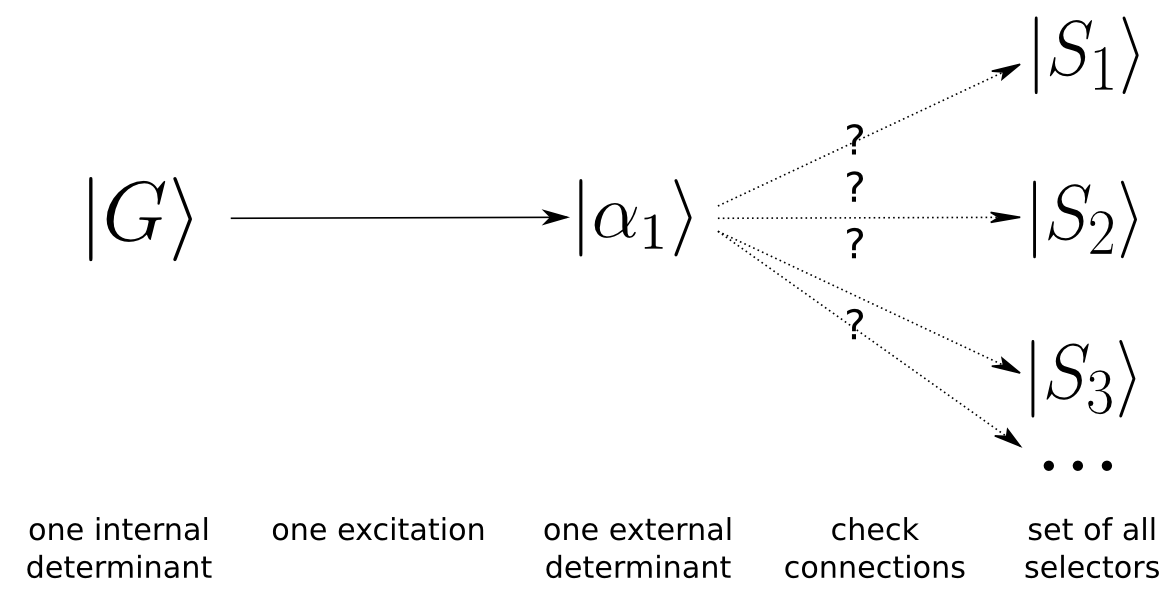
\includegraphics[width=0.6\columnwidth]{figures/cipsi/old_cipsi}
        \end{center}
        \caption{Original CIPSI schematic representation, some details omitted}
        \label{fig:old_cipsi}
\end{figure}


\begin{figure}[h!]
        \begin{center}
                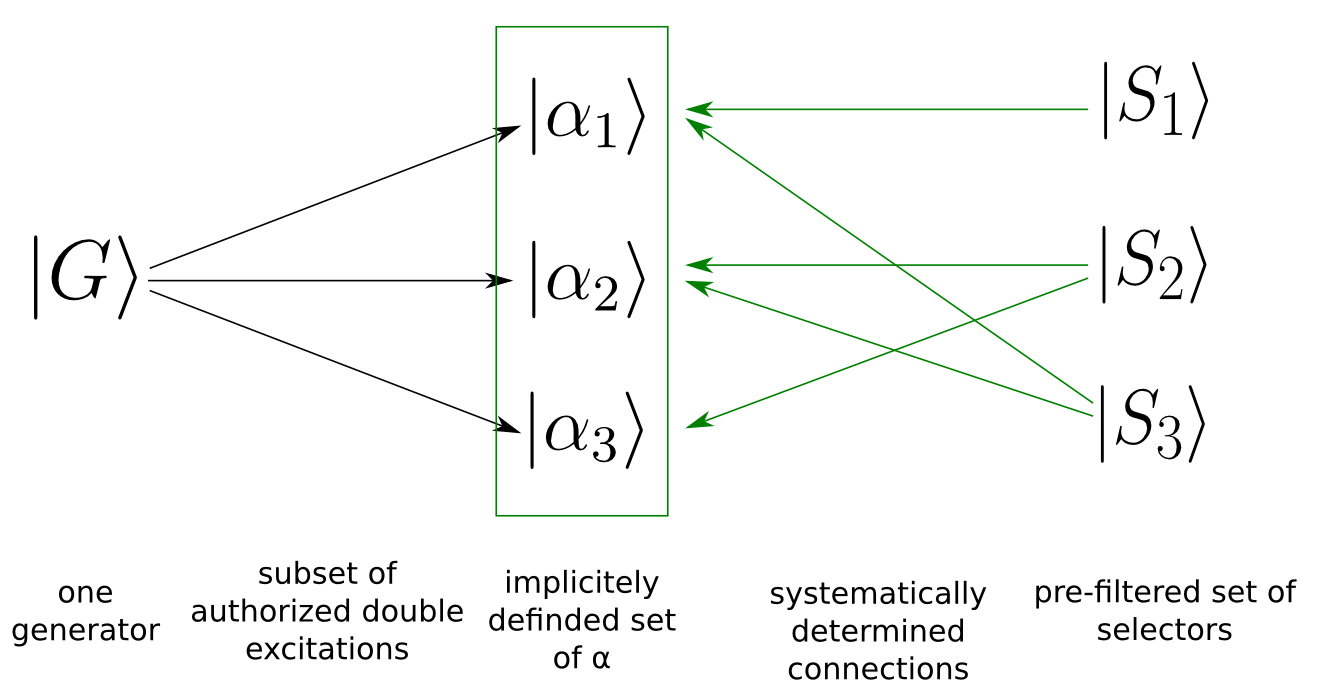
\includegraphics[width=0.6\columnwidth]{figures/cipsi/new_cipsi}
        \end{center}
        \caption{New CIPSI schematic representation, some details omitted.}
        \label{fig:new_cipsi}
\end{figure}

\subsection{Unfiltered algorithm}

Filtering of selectors is a somewhat natural idea that was actually implemented before the batch approach. It however can easily be understood as something added ``on top'' of it, so it will be detailed in the next section and ignored in this one.



\begin{enumerate}
%\setlength{\itemindent}{2em}
\item
Iterate over $\ket {G} \in \left \{ \ket{D_{I \leq \Ngen}} \right \}$.
\item
Iterate over all possible $a_p a_q \ket G = \ket {G_{pq}}$.
\item
Allocate a zero-initialized array for the matrix $P(G_{pq})$ indexed by $r$ and $s$. Each cell is associated with $\ordering a^\dagger_r a^\dagger_s a_p a_q  \ket G = \Gpqrs$. Some cells will be tagged as not being associated with a unique $\ket \alpha$, but either one of :
\begin{itemize}
\item
a determinant already present in the wavefunction
\item
an \emph{exclusion principle violating} determinant (EPV), i.e. $\Gpqrs = 0$
\item
a non-unique $\ket \alpha$ (either a double excitation of a previous generator, or a single excitation of the current one)
\end{itemize}

\item
Since two electrons cannot occupy the same spinorbital, tag cells where $r$ or $s$ is occupied in $\ket {G_{pq}}$ as well as those with $r=s$.
\item
Apply single excitation tagging. This ensures single excitations of $\ket G$ are generated exactly once. It is described in section \ref{single_tagging}.
\item
\textbf{selector loop}: Iterate over $\ket {S} \in \left \{ \ket{D_{J \le \Nsel}} \right \}$
\item
Determine whether there is an $(r,s)$ pair so that $\ket S = \ket {G_{pq}^{rs}}$. In other words, look for $\ket S$ in the current batch. If it is found, tag the corresponding cell, $\Gpqrs \in \{\ket{D_I}\}$.
\item
Determine $(r,s)$ pairs so that $\ket {G_{pq}^{rs}}$ is connected to $\ket S$
\item
If $J<I$, tag the corresponding cells ; $\Gpqrs$ is generated by $\ket{D_J}$.
\item
If $J \geq I$, increment all untagged $P_{rs}(G_{pq})$ matrix elements by $\Delta P_{rs}(G_{pq}) = c_J \Hij{S}{G^{rs}_{pq}}$. Note that the excitation operator $\hat{T}$ so that $\ket S= \pm \hat{T} \Gpqrs$, useful for computing the associated matrix element, can be determined at the same time as the $(r,s)$ pair.
\item
End \textbf{selector loop}. All untagged cells are guaranteed to be associated with a unique $\ket \alpha$ and $P_{rs}(G_{pq}) = \Hij{\Psi}{G^{rs}_{pq}}$. $e_\alpha$'s for the current batch can be computed, with $\kalpha = \ket {G_{pq}^{rs}}$, as
\begin{equation}
e_\alpha = \frac{P_{rs}(G_{pq})^2}{\Evar-\Hij{\alpha}{\alpha}}
\end{equation}
\item
End of other loops. All $e_\alpha$ have been computed a single time.

\end{enumerate}


\subsection{Tagging}

Tagged cells are simply tracked using a boolean matrix $B(G_{pq})$ with $B_{rs}(G_{pq})$ keeping the tag status of $\Gpqrs$, defaulting to $\FALSE$.
In some cases, full columns/rows are to be tagged. Keeping track of fully tagged rows or columns is useful for performance purpose, as it allows to bypass some loop iterations. A simple way to do it, is to add an extra column and an extra row of index $0$ to $B$ ; $B_{0s}(G_{pq}) = \TRUE\,$ means the whole $s$ column is tagged, $B_{r0}(G_{pq}) = \TRUE\,$ means the whole $r$ line is tagged. The actual tag status of $\Gpqrs$ becomes
\begin{equation}
B_{r0}(G_{pq}) \vee B_{0s}(G_{pq}) \vee B_{rs}(G_{pq}).
\end{equation}
While significant, this optimization is fairly simple to set up and use, so for simplification purpose, it will be ignored in the text.


\subsection{Single excitation tagging}
\label{single_tagging}
The algorithm is designed to generate all $\ket {G_{pq}^{rs}}$, which are doubly excited from $\ket G$. The singly excited determinants are not explicitly generated, but are formally present as $\ket{G_{pq}^{ps}}$.
The issue is that $\ket{G_{pq}^{ps}}$ refers to the same determinant $\ordering a^\dagger_s a_q \ket{G}$ regardless of $p$, and the base algorithm only tags a $\kalpha$ as duplicate if it can be generated by $\ket {D_{J < I}}$, i.e. if
\begin{equation}
\ket {G_{pq}^{rs}} = \ket {K_{p'q'}^{r's'}} \; ; \; \ket G = \ket{D_I} 
\end{equation}
As can be seen this doesn't cover the case where $\ket{G_{pq}^{ps}} = \ket{G_{p'q}^{p's}}$.

To solve this issue, we default to tag $\ket {G_{pq}^{ps}}$, which prevents generating single excitations, and selectively untag in certain cases:


\begin{itemize}
\item
\textbf{Untagging all $\uparrow$-spin single excitations of $\ket G$ exactly once}:

Pick $P$ any ``non-frozen'' $\downarrow$ spinorbital occupied in $\ket G$. We arbitrarily choose the lowest one. Untag $\ket {G_{Pq}^{Ps}}$ whenever $q,s$ are of $\uparrow$ spin. Any $\uparrow$-spin single excitation $q \rightarrow  s$ is untagged a single time.

$P$ cannot be chosen of $\uparrow$ spin, because single excitations $P \rightarrow  s$ and $q \rightarrow  P$ would be formally present as $\ket{G_{PP}^{Ps}}$ and $\ket{G_{Pq}^{PP}}$, which aren't ever generated, since for obvious reasons the base algorithm never considers the batch $\ket{G_{qq}}$ or the determinants $\ket {G_{pq}^{rr}}$.
\item
\textbf{Untagging all $\downarrow$-spin single excitations of $\ket G$ exactly once}:

Pick $Q$ any ``non-frozen'' $\uparrow$ spinorbital occupied in $\ket G$. Again we arbitrarily choose the lowest one. If $p,q$ are of $\downarrow$ spin, untag $\ket{G_{pQ}^{rQ}}$. Any $\downarrow$-spin single excitation $p \rightarrow  r$ is untagged a single time.
\end{itemize}



\section{Systematic determination of connections}

\begin{figure}[h!]
        \begin{center}
                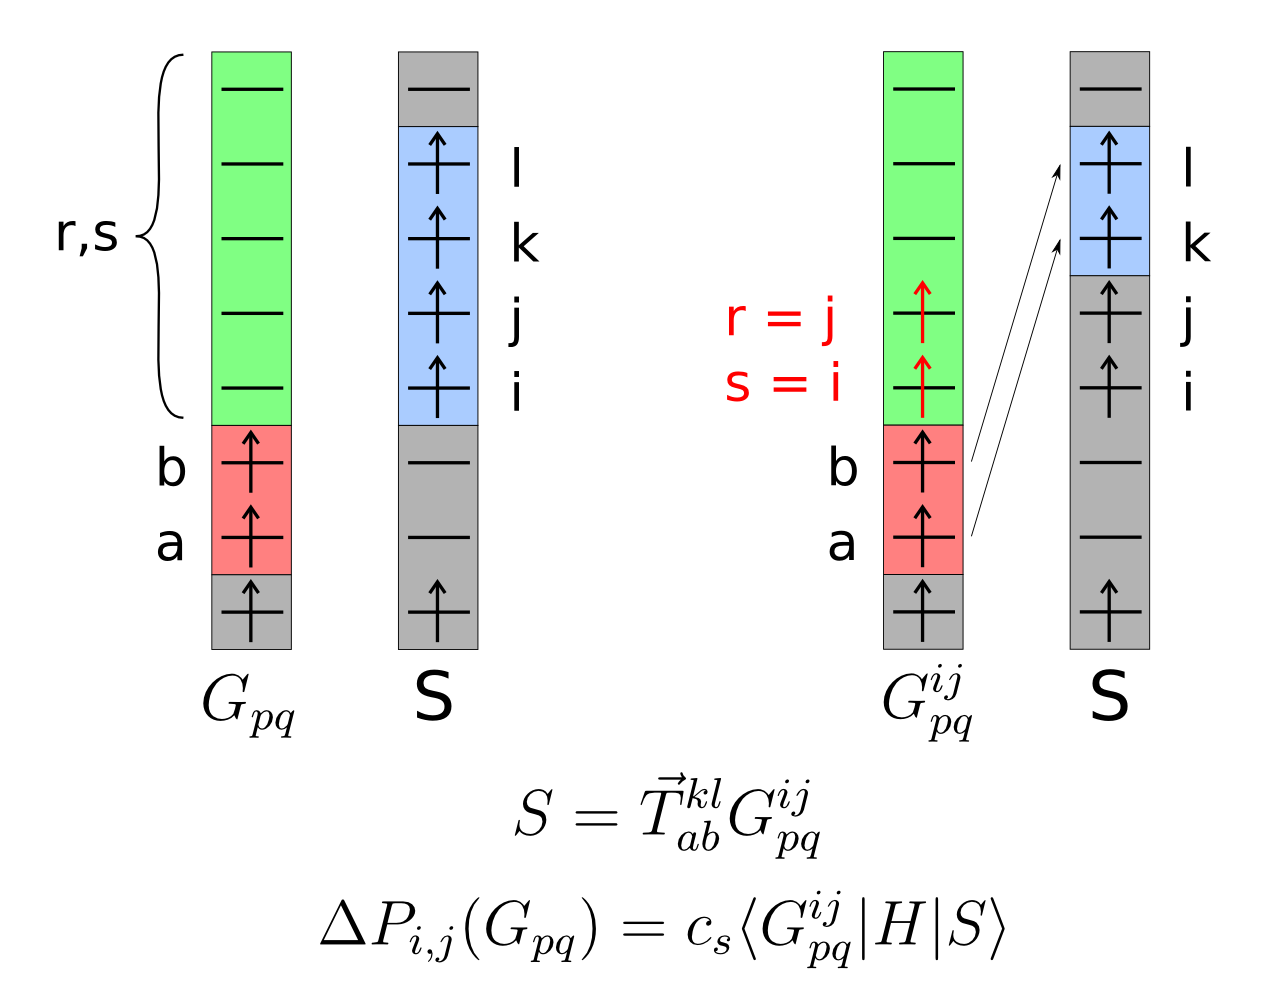
\includegraphics[width=0.70\columnwidth]{figures/cipsi/systematic_determination}
        \end{center}
        \caption{Illustrative example of systematic determination of the connection between a selector $\ket S$ and determinants of the $\ket {G_{pq}}$ batch when $p$ and $q$ have the same spin. $c_S$ is the coefficient of $\ket S$ in $\ket \Psi$.}
        \label{fig:systematic_determination}
        
\end{figure}


\begin{figure}[h!]
        \begin{center}
                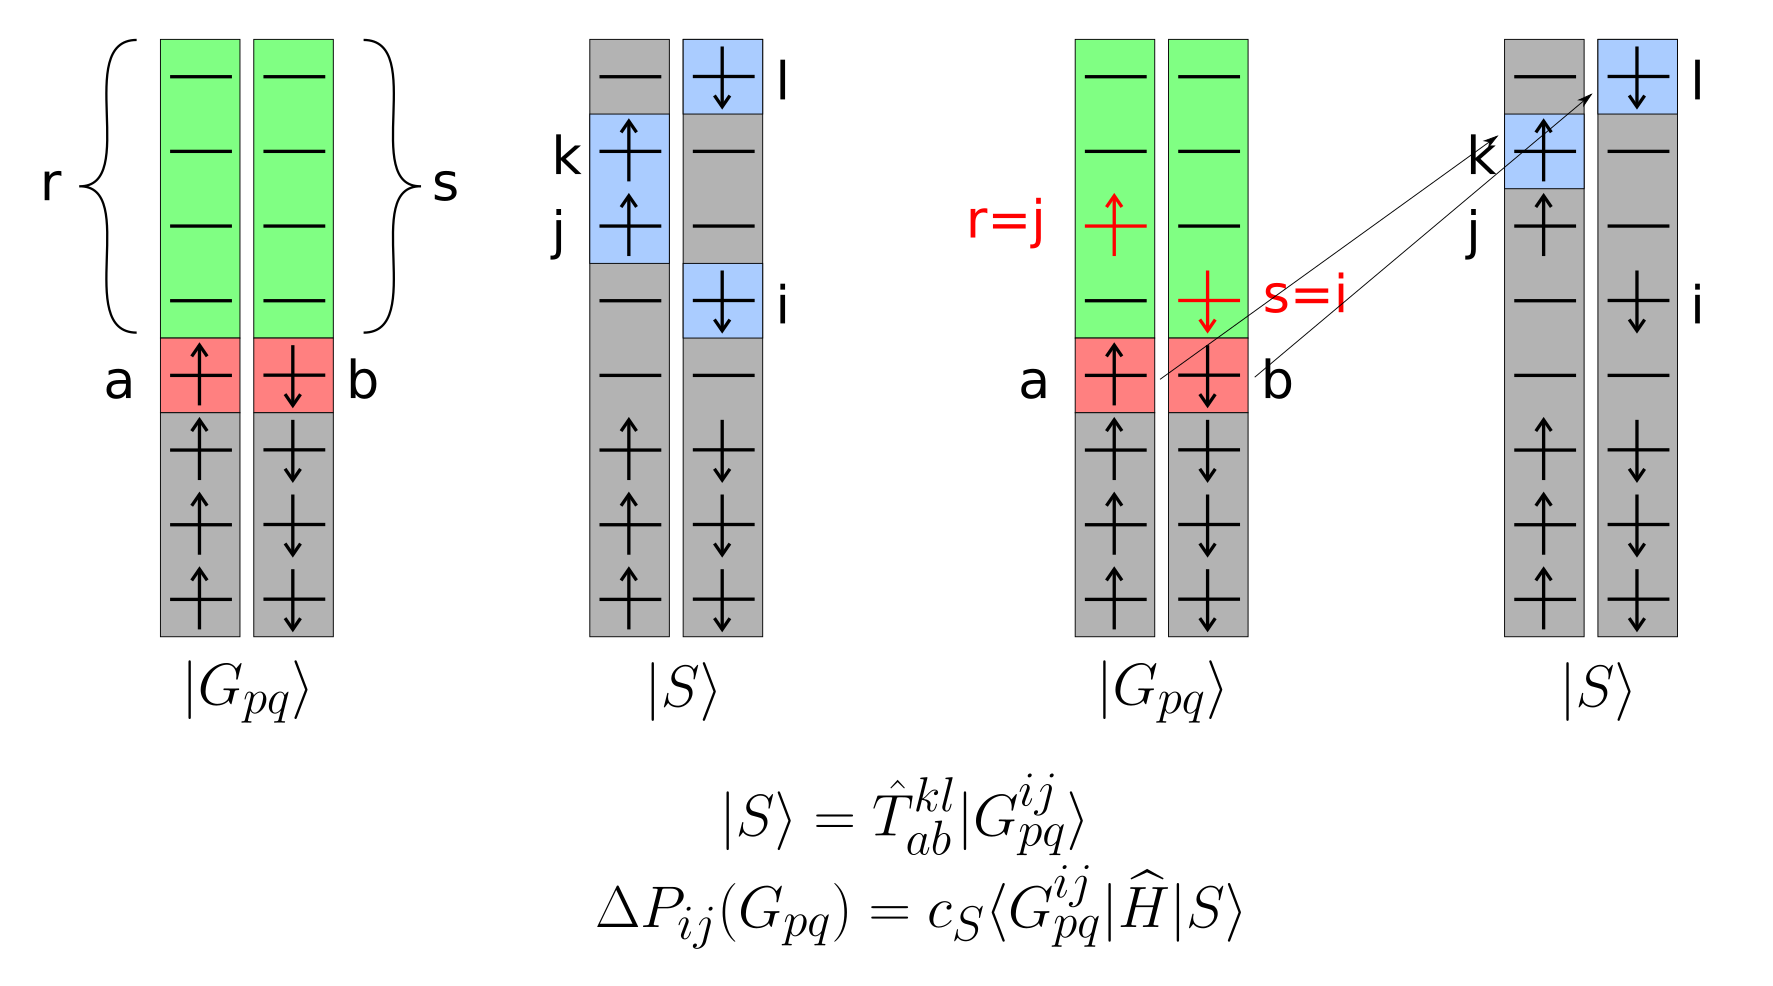
\includegraphics[width=0.90\columnwidth]{figures/cipsi/systematic_determination2}       
        \end{center}
        \caption{Illustrative example of systematic determination of the connection between a selector $\ket S$ and determinants of the $\ket {G_{pq}}$ batch when $p$ and $q$ are of different spins. $c_S$ is the coefficient of $\ket S$ in $\ket \Psi$.}
        \label{fig:systematic_determination2}
\end{figure}


The systematic determination of connections between $\ket S$ and determinants from the ${G_{pq}}$ batch is done by comparing $\ket S$ to the doubly ionized determinant $\ket {G_{pq}}$. This yields a set of spinorbitals whose occupation status differ. Remembering $\ket S$ has two extra electrons compared to $\ket {G_{pq}}$, there are 4 cases of interest:
\begin{itemize}

\item
$i$,$j$ are occupied in $\ket S$ but not in $\ket {G_{pq}}$
\item
$i$,$j$,$k$ are occupied in $\ket S$ but not in $\ket {G_{pq}}$ ; $a$ is occupied in $\ket {G_{pq}}$, but not in $\ket S$
\item
$i$,$j$,$k$,$l$ are occupied in $\ket S$ but not in $\ket {G_{pq}}$ ; $a$,$b$ are occupied in $\ket {G_{pq}}$, but not in $\ket S$
\item
More differences : $\ket S$ isn't connected to any $\ket {G_{pq}^{rs}}$ and can be ignored. 

\end{itemize}

Based on these indices, it is possible to immediately deduce any $(r,s)$ pair so that $\ket {G_{pq}^{rs}}$ is at most a double excitation of $\ket S$, as well as the excitation operator $\hat{T}$ so that $\ket {G_{pq}^{rs}}=\ordering \hat{T} \ket S$. Figures \ref{fig:systematic_determination} and \ref{fig:systematic_determination2} show two possible cases as examples.

While this could be done in a more compact way, we took a ``case by case'' approach, allowing more specialized code for each situation. Taking spin into account, the different cases are listed in table \ref{tab:systematic_determination}.


It is noticeable that, because of the ``wildcard'' indices $X$ and $Y$ :
\begin{itemize}

\item
Cases of the form $a,ijk$ cause full rows/columns of $P(G_{pq})$ to be tagged or incremented.
\item
Cases of the form $ij$ cause the whole $P(G_{pq})$ matrix to be tagged or incremented. Obviously, tagging the whole matrix means stopping the computation for ${G_{pq}}$.
\end{itemize}


\begin{algorithm}
        \caption{Unfiltered CIPSI selection}
        \label{alg:selection}
        \tcc{For simplification purpose, a determinant $\ket S$ is here represented by a single bitstring $S$ of size $2\Norb$ where each bit is associated with a spinorbital}
        \KwData{ $\ket \Psi$, i.e. $\{D_I\}$ the set of internal determinants and their coefficients $c_I$}
        \KwData{ $\Ngen$, $\Nsel$, $\Ndet$}
        %\KwResult{ $\Hij{\alpha}{\Psi} \neq 0$ has been computed exactly once for any $\alpha \notin \Psi$ }
        \KwResult{ $e_\alpha \neq 0$ has been computed exactly once for any $\kalpha \notin \{D_I\}$ }
                
        \For{$g \gets 1, \Ngen$}{
        \ForAll{$(p,q) \; ; \; a_p a_q \ket {D_g} \neq 0$}{
        	
                $\ket {G_{pq}} \gets \ordering a_p a_q \ket {D_g}$\;
                \tcc{$B$ and $P$ are indexed by spinrobitals}
                $B$ a $\FALSE$-initialized boolean matrix of size $2\Norb \times 2\Norb$ \;
                $P$ a zero-initialized real matrix size $2\Norb \times 2\Norb$ \;
                
                Apply EPV and single excitations tagging (algorithm \ref{alg:unblock_single}) \;
                
                \For{$t \gets 1,N_{det}$}{
                        $\ket S \gets \ket {D_t}$ \; 
                        $C \gets S \wedge \neg G_{pq}$ \; %c \gets \IAND{S}{\NOT{G_{pq}}}$ \; 
                        \If{$||C|| = 2$}{
                                $e \gets \texttt{LIST\_FROM\_BITSTRING}(C)$\; 
                                $B_{e[0]\, e[1]} \gets \TRUE$\;                     
                        }                       
                        \tcc{see table \ref{tab:systematic_determination} for $(r,s)$ pairs}
                        \uIf{$t < g$}{
                                    
                                \ForAll{$(r, s) \; ; \; \Hij{S}{G_{pq}^{r s}} \neq 0$}{
                                  $B_{rs} \gets \TRUE$ \;
                                } 
                        }
                        \ElseIf{$t \leq \Nsel$}{
                                \ForAll{$(r, s) \; ; \; \neg B_{rs} \wedge \Hij{S}{G_{pq}^{r s}}\neq 0 $ }{
                                  $P_{rs} \gets P_{rs} + c_t \Hij{S}{G_{pq}^{rs}}$ \;
                                }
                        }
                }
                \ForAll{$(r,s) \; ; \; \neg B_{rs}$}{
                  $\kalpha = \Gpqrs$ is a unique $\kalpha$ \;
                  $e_\alpha = \frac{{P_{rs}}^2}{\Evar - \Hij{\alpha}{\alpha}}$ \;
                  %$P_{rs}$ is $\Hij{G_{pq}^{rs}}{\Psi}$ \;
                }
        }
        } 
\end{algorithm}


\begin{algorithm}
        \caption{EPV and single excitations tagging}
        \label{alg:unblock_single}
        \KwData{$B$, $q$, $p$ and $\ket {G_{pq}}$ from outer scope. }
        \KwResult{Updates $B$ so as to tag EPVs, and determinants that are generated by a generator of lower index from a single excitation on $\ket G$}

        \tcc{tag EPV}
        \ForAll{$r$}{
        	$B_{rr} \gets \TRUE$ \;
        }
                \ForAll{$r \; ; \; (a_r \ket {G_{pq}} \neq 0) \vee (r=p) \vee (r=q)$}{
                        $B_{*r} \gets \TRUE$ \;
                        $B_{r*} \gets \TRUE$ \;
                }
        \tcc{tag duplicate single excitations}
                \If{($q$ is $\uparrow$) $\wedge$ ($p$ is the lowest ``non-frozen'' occupied $\downarrow$ spinorbital in $\ket G$)}{
                                $B_{*p} \gets \FALSE$ \;  
                                $B_{p*} \gets \FALSE$ \;          
                        }
                        
                        \If{($p$ is $\downarrow$) $\wedge$ ($q$ is the lowest ``non-frozen'' occupied $\uparrow$ spinorbital in $\ket G$)}{
                                $B_{*q} \gets \FALSE$ \; 
                                $B_{q*} \gets \FALSE$ \;         
                        }
\end{algorithm}



\section{Filtering and loop breaking}

A large amount of CPU time is wasted because every doubly ionized generator $\ket {G_{pq}}$ is compared to all internal determinants. In the vast majority of cases, it will show no connection can be made and the internal determinant will be ignored. Thus, it is interesting to filter internal determinants in the outermost loops (loop over generators, and loop over first ionization).

This can be done using the distance $f_A^B = f_B^A$, defined as the minimal number of operations ---~moving, annihilating or creating an electron~--- that must be done to go from a determinant $\ket A$ to a determinant $\pm \ket B$ (i.e. ignoring the phase factor) with respectively $n_A$ and $n_B$ electrons.
Alternatively, it can be defined as the maximum between the number of annihilations and the number of creations required to go from $\ket A$ to $\pm \ket B$.




\begin{equation}
f_A^B = \frac{\norm{A_\uparrow \oplus B_\uparrow} + \norm{A_\downarrow \oplus B_\downarrow} + |n_A-n_B|}{2}
\end{equation}


Considering $\ket S$ a selector determinant and $\ket X$ a generator determinant in a state of ionization from 0 to 2 (it essentially is a wildcard for $\ket G$, $\an p \ket G$ or $\an p \an q \ket G = \ket {G_{pq}}$).

\begin{itemize}
\item
$f_X^\alpha + f_\alpha^S \geq f_X^S$
\item
$\ket \alpha$ can be generated from $\ket X$ iff $f_X^\alpha \leq 2$
\item
$\ket \alpha$ is connected to $\ket S$ iff $f_\alpha^S \leq 2$
\item
$0 \leq \qty(f_Y^S - f_X^S) \leq 1$ with $\ket Y = a_p \ket X$
\end{itemize}


From the rules above, we can deduce that given any $\ket X$ and $\ket S$, there exists an $\kalpha$ generated from $\ket X$ so that $\Hij{\alpha}{S} \neq 0$ only if $f_X^S \leq 4$.
Based on this, a filtering mechanism can be set up, as shown on figure \ref{fig:selection}. The diagram is somewhat convoluted and deserves comments.

\paragraph{Internal determinants' path}
 
A triple loop is shown

\begin{enumerate}
\item
over generators $\ket G$
\item
over $p$ a first ionization $\ket{G_p}$
\item
over $q$ a second ionization $\ket{G_{pq}}$, i.e. over batches.
\end{enumerate}

In each one some filtering takes place. The internal determinants ``flow'' from the top $\{ \kI \}$ into intermediate lists, that are fully constructed before proceeding to the inner loop, as they will be the sources of determinants for that inner loop.
A selector can only be duplicated at the node denoted by a black circle. Otherwise, it follows a single path, always going for the horizontal path if it satisfies the associated condition.
If it doesn't satisfy the condition of a horizontal path, and there is no further vertical path, it is discarded.

\paragraph{``Drop'' instructions}
\emph{Drop} instructions are reached when, predictably, the current loop iteration will not yield any unique $\kalpha$. If a determinant reaches a \emph{drop}, the current loop iteration ends immediately.

\begin{itemize}
\item
\emph{drop} $G_{pq}$ is reached in the case where the whole $P(G_{pq})$ matrix is to be tagged, i.e. the possible values for $(r,s)$ given by table \ref{tab:systematic_determination} are two wildcards ($X,Y$ and $X,\bar Y$).
This corresponds to the case where $\ket {G_{pq}}$ has already been created from a previous generator $\ket K$, i.e. $\ket {G_{pq}} = \ket {K_{p'q'}}$, therefore for any pair $(r,s)$ we have $\ket {K_{p'q'}^{rs}} = \ket {G_{pq}^{rs}}$.\\
\item
\emph{drop} $G_{p}$, in the same fashion, is reached when $a_p \ket G = \ket {G_{p}}$ has already been created from a previous generator $\ket K$, i.e. $\ket {G_{p}} = \ket{K_{p'}}$. For any $(q,r,s)$ triplet there will be $\ket {K_{p'q}^{rs}} = \ket {G_{pq}^{rs}}$, so no new $\kalpha$ will be created.
\end{itemize}


\paragraph{Paths and loops}
There are roughly a left and a right path. The reason for this, is that we want to reach \emph{drop} instructions as fast as possible. Incidentally, in each loop, the implementation should prioritize operations that may cause a reach to \emph{drop}.

%Not trying to reach \emph{drop} $G_{PQ}$ means we might completely compute the $P$ matrix, only to find that the last selector determinant tags it entierly, for the reson mentioned above.
%Not trying to reach \emph{drop} $G_{P}$ means we might iterate over batches $\Gpqrs$ that are all to be "tagged out" by a single particular selector.

\begin{enumerate}

\item
The first loop discards some internal determinants and separates the others in two disjoint categories.


\begin{itemize}
\item
Right branch : determinants that may contribute to the $P(G_{pq})$ matrix or tag previously generated $\ket \alpha$. In other words, selectors that may connect to some $\ket {G_{pq}^{rs}}$. 

\item
Left branch : Determinants that aren't selectors, but are equal to some $\ket {G_{pq}^{rs}}$. Being non-selectors, those will not be checked for connection to any $\ket {G_{pq}^{rs}}$, but they still must be checked for equality in order to ensure $\ket {G_{pq}^{rs}} \notin \left \{ \kI \right \}$
\end{itemize}


This step sets the complexity of the algorithm with respect to $\Ndet$. Naively, $f_G^S$ must be computed for all pairs of internal determinants, setting the complexity to $\mathcal{O}(\Ndet^2)$.
\begin{comment}
\begin{algorithm}
\caption{Filtering internal determinants for generator $\ket G$}
\label{alg:generators_filtering}
\KwData{$U_\uparrow, U_\downarrow$~: the set of unique $\uparrow$ and $\downarrow$ strings used
to build the $\Ndet$ determinants. $\ket G$ a generator determinant.}
\KwResult{Finds all $\ket S$ internal determinants so that $f_G^S \leq 4$}
\For{$S_\uparrow \in \{U_\uparrow \}$}{
$a \gets \texttt{EXC\_DEGREE}(S_\uparrow, G_\uparrow)$ \;
\If{$a \leq 2$}{
        find $S_\downarrow \in \{U_\downarrow\}_{G_\uparrow}$ so that $\text{EXC\_DEGREE}(S_\downarrow, G_\downarrow) + a \leq 4$  \; 
}
}
\For{$S_\downarrow \in \{U_\downarrow \}$}{
$b \gets \text{EXC\_DEGREE}(S_\downarrow, G_\downarrow)$ \;
\If{$b \leq 1$}{
        find $S_\uparrow \in \{U_\uparrow \}_{G_\downarrow}$ so that $\text{EXC\_DEGREE}(S_\uparrow, G_\uparrow) + b \leq 4$  \; 
}
}
\end{algorithm}
\end{comment}

\begin{algorithm}
\caption{Filter internal determinants $\ket S$ so that $f_G^S \leq 4$ }
\label{alg:generators_filtering}
\KwData{$\ket G$: a generator determinant.}
\KwData{$\Nalphadet$: the number of unique $\uparrow$ spin parts present in $\ket \Psi$.}
\KwData{$D^\uparrow$: the array of determinants present in $\ket \Psi$, sorted by $\uparrow$-major order (all determinants sharing the same $\uparrow$ part are next to each other).}
\KwData{$A^\uparrow$: the arrays so that $A^\uparrow[n]$ is the index of the first occurence of the $n^{th}$ unique $\uparrow$ spin part in $D^\uparrow$. For algorithmic convenience we set $A^\uparrow[\Nalphadet +1] = \Ndet+1$.}
\KwData{$\Nbetadet$, $D^\downarrow$, $A^\downarrow$: the $\downarrow$ counterparts.}

\For{$a \gets 1, \Nalphadet$}{
$e \gets \text{EXC\_DEGREE}(D^\uparrow[A^\uparrow(a)]_\uparrow, G_\uparrow)$ \;
\If{$e \leq 2$}{
	\For{$b \gets A^\uparrow(a), A^\uparrow(a+1)-1$}{
		\If{$e + \text{EXC\_DEGREE}(D^\uparrow[b]_\downarrow, G_\downarrow) \leq 4$}{
			retain $D^\uparrow[b]$ \;		
		}
	}
}
}

\For{$a \gets 1, \Nbetadet$}{
$e \gets \text{EXC\_DEGREE}(D^\downarrow[A^\downarrow(a)]_\downarrow, G_\downarrow)$ \;
\If{$e \leq 1$}{
	\For{$b \gets A^\downarrow(a), A^\downarrow(a+1)-1$}{
		\If{$e + \text{EXC\_DEGREE}(D^\downarrow[b]_\uparrow, G_\uparrow) \leq 4$}{
			retain $D^\downarrow[b]$ \;		
		}
	}
}
}
\end{algorithm}

Our current implementation quickly discards $f_G^S > 4$ by using a method similar to what we used in the Davidson diagonalization, adapted to seek excitation degrees $\leq 4$ rather than $\leq 2$. The key difference is that, for parallelism reasons, the research has to be done individually for each generator~; that is, we are not computing all $f_G^S$ at the same time, but all $f_G^S$ for a given $\ket G$ separately. The procedure is shown as algorithm \ref{alg:generators_filtering}. The complexity is reduced from $\order{\Ndet^2}$ to $\order{\Ndet^{3/2}}$.




Note that the only point of separating those two categories rather than merging them in the same list, is to avoid additional \emph{past} and \emph{selector} tests in the second loop.
%If both those lists were merged, a $selector$ condition would need to be added for reaching the right list of the second loop, and $past$ tests would be performed pointlessly on those determinants that would have gone in the left list of the first loop.
This most likely is of little interest, depending on the implementation.
%$past$ and $selector$ should at worst mean fetching an index in an array of indices, and compare it to $D_I$ or $N_{sel}$ respectively.
But because it is the actual implementation and because it reduces the number of operations, it is still shown.

\item
The second loop discards some internal determinants and separates the other in two categories, this time not disjoint.

\begin{itemize}
\item
Right branch : Selectors that may connect to some $\Hij{\Psi}{\alpha}$.
\item
Left branch : Determinants that may be equal to some $\ket {G_{pq}^{rs}}$. Those can be found in both lists built in the first loop.
\end{itemize}

As previously discussed, if there is a previous generator $\ket K$ so that $a_{p'} \ket K = a_p \ket G$, it will result in $P(G_{pq})$ being fully tagged for any $q$, hence a need to reach \emph{drop} $G_p$ to avoid unnecessary computations.
The reach for \emph{drop} $G_p$ can be put on the path between the right list of the first loop and the left list of the second loop.

Indeed, $a_{p'} \ket K = a_p \ket G$ with $\ket K$ a previous generator translates to
\begin{equation}
\qty(f^K_{G_{p}} = 1) \wedge \text{past}
\end{equation}
The right list of the first loop contains all internal determinants so that
\begin{equation}
\qty(f^K_G \leq 4) \wedge \text{selector}
\end{equation}
However 
\begin{equation}
f^K_{G_{p}} = 1 \implies f^K_G \leq 1 \implies f^K_G \leq 4
\end{equation}
\begin{equation}
\text{past} \implies \text{selector}
\end{equation}
\begin{equation}
\qty(f^K_{G_{p}} = 1) \wedge \text{past} \implies\qty (f^K_G \leq 4) \wedge \text{selector}
\end{equation}

Therefore any internal determinant able to reach \emph{drop} $G_p$ will be present in that list. Trivially, from there it will always take the left path because $f^K_{G_{p}} = 1 \implies f^K_{G_{p}} \leq 2$.


\item
Third loop :
\begin{itemize}

\item
Right branch :
Final filtering to keep only selectors that do connect to some $\Gpqrs$
\item
Left branch : $f_{G_{pq}}^S = 2$ implies there exists $(r,s)$ so that $\ket S=\Gpqrs$. When one is found :
\begin{itemize}
\item
If $\text{past}$
\begin{equation}
\ket S=\ket {G_{pq}^{rs}} \implies \ket {S_{rs}} = \ket {G_{pq}}
\end{equation}
As explained above, it leads to $P(G_{pq})$ being fully tagged, and thus \emph{drop} $G_{pq}$ can be reached.
\item
If $\neg \text{past}$, $\ket {G_{pq}^{rs}}$ must be tagged for referring to a determinant of the internal space.
\end{itemize}



\end{itemize}

\end{enumerate}



\newcommand{\Gpq}{\ket {G_{pq}}}
\newcommand{\Gpbq}{\ket {G_{p \bar q}}}

\begin{table}

\caption{Systematic ``case by case'' determination of connections between a selector $\ket S$ and determinants of a batch $G_{pq}$} 
\label{tab:systematic_determination}
\begin{center}
\begin{minipage}[l]{0.6\textwidth}
        \begin{tabular}{ c|c|c }
                \hline \hline \rule{0pt}{3ex}
                $\ket S$                                                                        &$ r, s$        & $\hat T$ such that $\hat T \ket S = \pm \Gpqrs$     \\
                \hline \hline \rule{0pt}{3ex}
                $\ac {ij} \Gpq$                                         & $X,Y$         &$ij \rightarrow XY$            \\
                                                                                        & $X,i$         &$j \rightarrow X$              \\
                                                                                        & $i,j$         &$\hat 1$                    \\
                \hline \rule{0pt}{3ex}
                $\an a \ac {ijk} \Gpq$                          &$X,i$          &$aX \rightarrow jk$            \\
                                                                                        &$i,j$          &$a \rightarrow k$              \\
                \hline \rule{0pt}{3ex}
                $\an {\bar a} \ac {\bar i jk} \Gpq$     &$X,j$          &$\bar a k \rightarrow \bar i X$                \\
                                                                                        &$j,k$          &$\bar a \rightarrow \bar i$            \\
                \hline \rule{0pt}{3ex}
                $\an {ab} \ac {ijkl} \Gpq$                      &$i,j$          &$ab \rightarrow kl$            \\
                \hline \rule{0pt}{3ex}
                $\an {a  \bar b} \ac {ijk \bar l} \Gpq$                 &$i,j$          &$a \bar b \rightarrow k \bar l$                \\
                \hline \rule{0pt}{3ex}
                $\an {\bar a \bar b} \ac {i j \bar k \bar l} \Gpq$      &$i,j$          &$\bar a \bar b \rightarrow \bar k \bar l$              \\
                
                \hline \hline \rule{0pt}{3ex}
                $\ket S$                                                                        &$ r, \bar s$   & $\hat T ; \hat T \ket S = \ket {G_{p \bar q}^{r \bar s}}$     \\
                \hline \hline \rule{0pt}{3ex}
                $\ac {i \bar j} \Gpbq$                          & $X, \bar Y$   &$i \bar j \rightarrow X \bar Y$                \\
                                                                                        & $i,\bar X$            &$\bar j \rightarrow \bar X$            \\
                                                                                        & $X,\bar j$    &$i \rightarrow X$              \\
                                                                                        & $i,\bar j$    &$\hat 1$                    \\
                                                                                        
                                                                                        
                \hline \rule{0pt}{3ex}
                $\an a \ac {ij \bar k} \Gpbq$           &$X,\bar k$             &$aX \rightarrow ij$            \\
                                                                                        &$i,\bar k$             &$a \rightarrow j$              \\
                                                                                        &$i,\bar X$             &$a \bar k \rightarrow j \bar X$                \\
                                                                                        
                \hline \rule{0pt}{3ex}
                $\an {ab} \ac {ijk \bar l} \Gpbq$                       &$i,\bar l$             &$ab \rightarrow jk$            \\
                \hline \rule{0pt}{3ex}
                $\an {a  \bar b} \ac {ijk \bar l} \Gpbq$                        &$i,j$          &$a \bar b \rightarrow k \bar l$                \\
                \hline \rule{0pt}{3ex}
                $\an {a  \bar b} \ac {ij \bar k \bar l} \Gpbq$                  &$i,\bar k$             &$a \bar b \rightarrow j \bar l$                \\
        \end{tabular} 
\end{minipage}
\begin{minipage}[r]{0.3\textwidth}
\begin{itemize}
\item
the bar notation $\bar a$ is used to indicate relative spins
%, i.e. $ab$ means $a$ and $b$ are of same spin, $a\bar b$ means they are of different spin.
\item
$\an{ij\ldots}$ is a compact notation for $\an i \an j \ldots$
\item
$X$ and $Y$ are ``wildcard'' indices referring to any spinorbital unoccupied in both $\ket S$ and $\ket {G_{pq}}$ 
\end{itemize}
%- "is in wavefunction" : $\ket {G_{pq}^{rs}} = S$. There is no need to compute $\langle \ket {G_{pq}^{rs}}|H|S \rangle$ since $\ket {G_{pq}^{rs}}$ is necessarily tagged for being present in the wavefunction.
\end{minipage}
\end{center}
\end{table}


\begin{figure}[h!]
        \begin{center}
                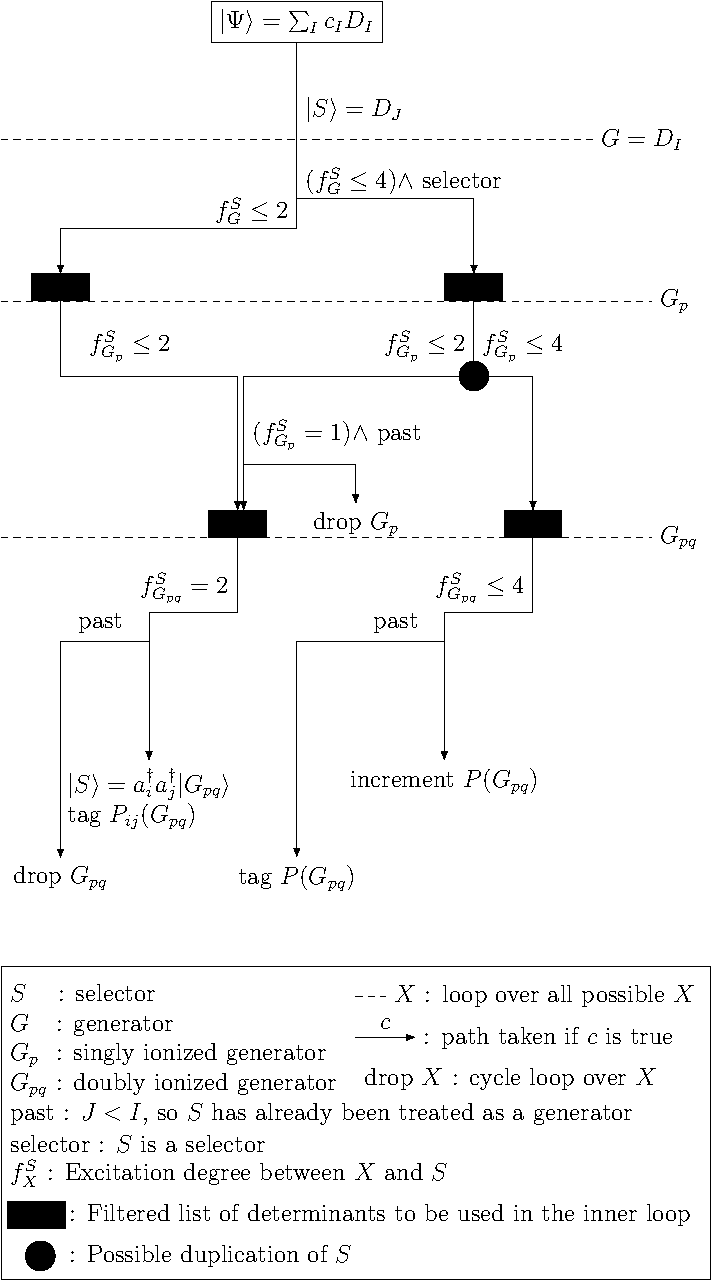
\includegraphics[height=0.90\textheight]{figures/cipsi/selection}
        \end{center}
        \caption{$\ket S$ is the internal determinant currently flowing down the chart.
        Tagging is fully computed, and \emph{drop} instructions eventually reached before any update is done to $P(G_{pq})$.}
        \label{fig:selection}   
\end{figure}

\clearpage
\section{Parallel computation}

Arguably the simplest way to make an algorithm parallel is, whenever possible, to create independent tasks corresponding to one iteration of the outermost loop.
As figure \ref{fig:selection} suggests, iterations for the outermost loop --- over generators --- are independent. This is due to our choice to perform the initial filtering on a ``generator by generator'' basis (algorithm \ref{alg:generators_filtering}). The cost for this initial filtering could be reduced with a ``spin part by spin part'' basis as in our Davidson algorithm, but since the CIPSI selection is more expensive than the Davidson diagonalization, the filtering steps only account for a few percent of the total CPU time, so for simplicity and load balancing we stuck to 1 task = 1 generator. Even so, the cost for different tasks is still very much unbalanced, the first few generators with large coefficients being very expensive, and the cost quickly decreasing.

For a better load balancing, we split the first, expensive tasks into smaller \emph{fragments}, using a fairly simple approach. Essentially, some tasks will require computing just a subset of the ${G_{pq}}$ batches associated with a generator $\ket G$, as opposed to all of them. This implies some overhead, since some filtering steps will be duplicated. Fortunately, only a relatively small number of expensive tasks need to be split.


Each generator $\ket {D_i}$ defines as a ``logical'' task $i$, and for each one we define $F_i$ a fragmentation level, defining the number of independent ``actual'' tasks it should be decomposed in.
We have empirically chosen the following expression for the fragmentation of the tasks:
\begin{align}
F_{\max} & = 1 + \min \qty( \Nelec (\Nelec-1)/2, \lfloor \sqrt{\Nsel} \rfloor/10 ) \\
F_i & = 1 + F_{\max} \qty( \max_{k=1}^{\Nst} |c_{ik}|^{1/2} )
\end{align}
where $F_i$ is an estimated cost of task $i$. In practice $F_i = 1$ for the majority.

Task $i$ is put in the task queue $F_i$ times, each time associated with a `fragment'' index $s$ ranging from $0$ to $F_i-1$, which together with $F_i$ defines the subset of batches this task corresponds to.
%Disjoint subsets are created using modulus, so that subsets are interleaved and thus more balanced.
% Cette phrase n'etait pas facile a comprendre. Le plus simple, c'etait de la virer...
 
\begin{algorithm}
        \caption{Task splitting, pseudocode for master}
        \label{alg:tasksplit_master}
        \tcc{A logical task is the computation of $e[i]$, the sum of $e_\alpha$ over all unique $\kalpha$ generated from generator $\ket {D_i}$}
        choose $F_i$ for all $i$\;
        \For{$i\gets 1,\Ngen$}{
        \For{$s\gets 0,F_i-1$}{
                add task $(i,s)$ to the queue   
        }
        }
        $f$,$e$ are arrays size $\Ngen$ initialized with $0$ \;
        \While{not all $e[i]$ printed}{
                get $(i,\text{sum})$ from a slave \;
                $e[i] \gets e[i] + \text{sum}$ \;
                $f[i] \gets f[i] + 1$ \;
                \If{$f[i] = F_i$}{
                        print $e[i]$ \;
                }
        }
\end{algorithm}

\begin{algorithm}
        \caption{Task splitting, pseudocode for slave}
        \label{alg:tasksplit_slave}
        \While{}{
                get task $(i, s \in [0,F_i-1])$ from the queue \;
                $E \gets 0$ \;
                $c \gets 0$ \;
                $G \gets D_i$ \;
                \tcc{duplicated computation if $F_i > 1$}
                filtering for $G$ (see figure \ref{fig:selection}) \;
                \ForEach{$G_p$}{
                \tcc{duplicated computation if $F_i > 1$}
                filtering for $G_p$ (see figure \ref{fig:selection}) \;
                \ForEach{$G_{pq}$}{
                        $c \gets c + 1$ \;
                        \If{$s = c \mod F_i$}{
                                increment $E$ with all unique $e_\alpha$ in this batch \;
                        }
                }
                }
                send $(i, E)$ to master \;
        }
\end{algorithm}

This fragmentation scheme can be shown in a simpler and more general way when used to compute $\EPT$ in chapter \ref{chap:PT2}. In a nutshell, we can see it as a toy problem where we want to print for each generator the sum of $e_\alpha$ over all unique $\kalpha$ it has generated. The algorithms for this on the master side and slave side are shown as algorithms \ref{alg:tasksplit_master} and \ref{alg:tasksplit_slave} respectively.


For the determinant selection, we still use the mixed MPI/OpenMP paradigm, where one MPI process per node is used for efficient broadcasting of the replicated data. But, as opposed the Davidson implementation where each task was parallelized with OpenMP, here each OpenMP thread handles independently a task, computed with a single core. The first reason is that the number of tasks is larger than $\Ndet$, which is usually orders of magnitude larger than the number of CPU cores. Moreover, the computation of a task in parallel would require a synchronization barrier at the beginning and the end of the OpenMP section. Here, all the OpenMP threads are completely independent during the whole calculation of the selection, and this explains the very good scaling properties of the implementation, as shown in chapter~\ref{chap:PERF}.

\section{Obtaining spin-pure states}
\label{sec:cipsi_s2}

The presented algorithm generates a wavefunction which is expressed on a truncated space of Slater determinants. Determinants are not necessarily eigenfunctions of the $\widehat S^2$ operator, so the eigenfunctions of the truncated Hamiltonian are not guaranteed to be also eigenfunctions of $\widehat S^2$.

A conventional solution to avoid this issue is to work in the basis of \emph{Configuration State Functions} (CSFs). These are linear combinations of determinants which are eigenfunctions of $\widehat S^2$, and with the desired eigenvalue. Diagonalizing $\widehat H$ in this basis ensures that the solution is spin pure.

Working with CSFs instead of determinants has the additional advantage that the space of CSFs is smaller than the space of determinants. CSFs could in principle be used for CIPSI, but that makes the computation of the matrix elements of $\widehat H$ less straightforward.

We have chosen a more practical solution.\cite{Bytautas_2009} After the selection step, we add to the variational space all the determinants that are necessary to obtain a spin pure solution. These determinants correspond to all the possible spin flips in open shell determinants with the constraint that $\Nalpha$ and $\Nbeta$ are constant. The diagonalization of $\widehat H$ will automatically yield spin pure eigenfunctions at the cost of increasing the size of the wavefunction with many determinants with very small weights.

\section{Conclusion}

The novel implementation of the CIPSI algorithm runs orders of magnitude faster than the former one thanks to several key improvements.
\begin{itemize}
\item
Excitations do not need to be computed explicitly using algorithms such as those presented in chapter \ref{chap:DET_DRIVEN}. However the associated phase factors still have to be computed.
\item
Although not directly related to the CIPSI algorithm, the computation of the phase factors has been made much cheaper thanks to the use of phase masks (see section~\ref{chap:PHASEMASK}).
\item
Selector determinants are simultaneously compared to $\qty(\Norb-\Nalpha)^2$ external determinants $\kalpha$ thanks to the batch approach.
\item
Selector determinants go through a filtering mechanism that narrows down the number of selector determinants to be considered against a particular $\kalpha$ (a particular batch of $\kalpha$).
\end{itemize}

This made way for applications that were not affordable before, such as those presented in chapter~\ref{chap:APPLICATIONS}, as well as an additional application to copper complexes.\cite{1806.05115}
The algorithms presented in this chapter also lead to the methods presented in the next chapters.

\end{document}


\chapter{PT2}
\minitoc
\documentclass[./thesis.tex]{subfiles}

 
\begin{document}

\section{def}

\section{PT2 vs CIPSI}

CIPSI and PT2, all approximations aside, both imply computation of all $\epsilon(\alpha)$, so both can be computed at the same time. CIPSI is about identifying the set of the largest ones, PT2 is about computing the sum over all of them. There are two main consequences to this
\paragraph{PT2 is one iteration behind CIPSI}
In a practical sense, CIPSI is ahead of PT2. A iteration $n$, identifiying the most significant $\ket \alpha$ is about building $\Psi^{n+1}$ while summing them is about estimating the cost of truncation for $\Psi^{n}$. Computing PT2 for a "final" wavefunction therefore requiers an extra iteration, which applies to a larger $\Psi$ and thus is more costly. ( autres implementation de PT2 possible ).

\paragraph{CIPSI can take more approximations}
Fully computing the sum has to be more costly than just identifying the greatest terms. As was said in SELECTION, the CIPSI algorithm can take pretty drastic approximations%, because we only try to identify the set of $\ket \alpha$ with the largest contributions $\epsilon(\alpha)$.
	\begin{itemize}
		\item{$t_g$}
		allows to explore a reduced subset of $\ket \alpha$ in which we are almost sure to find those of interest.
		\item{$t_s$}
		allows for a less accurate and less expensive computation of $\epsilon(\alpha)$, which is unlikely to significantly change the identified set.
	\end{itemize}
	These approximations do not apply when computing PT2. The very large number of smaller contributions makes them much harder to neglect. Unfortunately, increasing $t_g$ and $t_s$ thresholds dramatically increases the computational cost.


\paragraph{}

Unfortunately, a partial computation of PT2 results in a biased value. Since $\epsilon(\alpha)$ is an energy contribution, it's necessarily negative, and PT2 is a sum of same-sign contributions. Therefore, truncating it inevitably results in a bias, some energy is missing but there is little clue how much exactly. The $t_g$ and $t_s$ thresholds used in CIPSI can be seen as ways of minimizing this truncation's amplitude for a given computational cost.

Before the stochastic computation of PT2 was set up, our best choice was to set low thresholds for $t_g$ and $t_s$ while performing CIPSI and accept very approximated values for PT2 of intermediary wavefunctions ; then, once the selection was completed, we would highen them just for a final, very costly ``PT2 only'' iteration. In fact, an exact computation with $t_g=N_{gen}$ and $t_s=N_{det}$ was often prohibitively long, so the final PT2 was still biased. 


We eventually solved this problem by turning the bias into an error bar. The base idea is that, instead of trying to get the largest possible chunk of contribution, we can randomly pick $\epsilon(\alpha)$ contributions and make a Monte-Carlo estimate for the sum over all $\ket \alpha$. In this case, to avoid any bias we must set

$$t_g = N_{gen} ; t_s = N_{det}$$

Not only the estimate will be unbiased and much closer to the actual PT2, but we will have an estimate for the error. Because PT2 is itself used as an approximation

$$E_{var} + E_{PT2} \simeq E_{fullCI}$$

An error significantly smaller than the typical accuracy of $E_{var} + E_{PT2}$ VS $E_{fullCI}$ is certainly acceptable.


For different reasons, the actual Monte-Carlo computation is significantly more convoluted than simply drawing random $\ket \alpha$.


\section{The sample space}


\paragraph{Initial note : ``Sample'' and ``Comb''}
Because of its original nature, this algorithm casts some ambiguity on what should be refered to as a ``sample''. We are going to estimate a sum of elementary contributions $E(I)$, compute and store them individually, and draw them based on a repartition function ; therefore they will be refered to as the \emph{samples}. But the values actually treated as samples in the statistical sense, are sums over several $E(I)$, refered to as \emph{combs}.




\paragraph{$\epsilon(\alpha)$ are packed into elementary contributions $E(I)$}
Individual $\epsilon(\alpha)$ are expensive to compute. In the CIPSI algorithm, each generator determinant creates a number of unique $\alpha$, and computes $\epsilon(\alpha)$ for each one of them.
Essentially, $\ket \alpha$ are grouped in $N_{gen}$ disjoint sets, each associated with a generator determinant, as shown in figure \ref{fig:mu_sample}.

	$$\epsilon(\alpha) \in \mathcal{A}_i ; \Hij{\alpha}{\Psi_i} \neq 0 ; \Hij{\alpha}{\Psi_{j<i}} =0 $$

Because of the numerous tricks used, we can compute all $\epsilon(\alpha)$ from one set considerably faster than if we had to compute each one separately. Therefore, in order to access a larger chunk of data, the stochastic PT2 algorithm will not consider individual $\epsilon(\alpha)$, but instead sums of all $\epsilon(\alpha)$ from the same set.
The elementary contributions we are considering, aren't $\epsilon(\alpha)$, but
	$$E(I) = \sum_{\alpha \in \mathcal{A}_I} \epsilon(\alpha)$$
Indeed
    $$E_{PT2} = \sum_{I} E(I)$$
    
$E(I)$ are already explicitely computed by our CIPSI implementation, which returned the aggregated values of $\epsilon(\alpha)$ for one job, one job being essentially a generator determinant.

\paragraph{$E(I)$ can be stored to avoid re-computation}
Each elementary contribution is associated with a generator determinant, so there are only $N_{gen}$ elementary contributions. This is small enough so, when a $E(I)$ contribution is computed, its value can be stored and simply re-used if the same sample is drawn again. This, in turn, means the exact result will eventually be known once every sample has been computed. The cost for this will essentially be the same as that of the purely deterministic computation, with a negligible additional cost due to the Monte-Carlo related computations ( drawing random numbers, finding the associated samples... ).

\paragraph{The sample space is divided in $N_{teeth}$ \emph{teeth}}
	Generator determinants are sorted with decreasing absolute values of $C_I$.
	As can be seen in figure (pas mise dans le git), the values of $E(I)$ span many orders of magnitude and decrease rapidly with $I$, in an exponential-ish way. Smoothed values for $E(I)$ are shown in figure \ref{fig:p_i}. There are a few reasons for that.
\begin{itemize}
	\item
	The values for the denominator $\Delta E_\alpha$ used in the computation of $\epsilon(\alpha)$ tend to increase, as variational determinants tend to be more and more excited and to populate higher orbitals ( detailler ? )
	\item
	The number of unique $\ket \alpha$ per generator decreases. Indeed, the more ``previous generators'' there is, the likelier it is that a generated $\ket \alpha$ was generated before.
	\item
	Unique $\ket \alpha$ are, by construction, disconnected from all previous generators, which mean they connect to a smaller and smaller norm of $\Psi$ ( see figure \ref{fig:a_con} ). 
\end{itemize}
It is not ideal for a Monte-Carlo computation to deal with sample values that span many orders of magnitude. A repartition function can alleviate the issue to some extent.
The last reason given for the decrease of $E(I)$ is the most important one, and leads us to consider
$$\tilde w_i = C_i^2$$
as a repartition function for $E(I)$ (detailler un poil). This is however not the exact repartition function used in the Monte-Carlo scheme. We will later introduce some slight modifications to it, for algorithmic reasons.

As can be seen in figure \ref{fig:eici2}, $$p_I = \frac{E(I)}{C_I^2}$$ is  still similar to $E(I)$ in that it spans orders of magnitude and overall decreases.
It follows that values in a small range of $p_I$ are relatively close. The entire space of $p_I$ is split in $N_{teeth}$ ranges refered to as \emph{teeth}. In figure \ref{fig:p_i}, the space of $p_I$ has been split in four teeth $P_1$ to $P_4$. The variance inside each tooth is expected to be, quite clearly, much smaller than the variance for the whole space.

As a matter of fact, the values actually sampled, are sums of 1 sample taken in each subspace, so-called ``combs''.
Essentially, the sum of ``one large, one average and one small'' has a lower variance than the sum of ``three at random''.

<formule qui permet de tout parfaitement comprendre un un clin d'oeil>


\paragraph{fully-computed teeth are moved to a ``deterministic'' part}


Because $E(I)$ decreases rapidly, most of the contribution is contained in the first samples. We can entierely compute the first samples, and only make a stochastic estimation for the sum of the smaller ones. This effectively splits $E(I)$ in two ranges, a deterministic one, then a stochastic one (hence the hybrid characteristic of this method), and our estimated energy

$E = E_D + E_S$

with $E_D$ the exact energy for the deterministic part, and $E_S$ the estimated energy of the stochastic part. The error bar only applies to $E_S$, which is a fraction of the whole sum.
We have to define the threshold between those two ranges. A simple solution would be to arbirarily define it based on $c_I$.
But because we have already defined ranges as teeth, we take a dynamical, more flexible approach : given the first $E(I)$ whose value is unknown (that has not been drawn yet by the Monte-Carlo scheme), and $P$ the tooth it belongs to, the deterministic range extends to $P$, exclusive.

\section{Practical considerations}

There are a few more practical details that must be dealt with.

\subsection*{initial deterministic part}

For each comb, we draw a sample $E(I)$ in each teeth. When a tooth is entirely computed, it is moved to the deterministic part. Thus, it is immediately obvious that a tooth containing a single sample makes no sense, as it will be instantly moved to the deterministic part ; it can as well be considered part of it. Because it's usually accepted (???) that it takes at least 30 samples to estimate a variance, we can go further and consider that a tooth with fewer than 5-10 samples will be moved to the deterministic part too fast to be of real interest. In fact because of the "tooth filling" mechanism described later on, we know the first tooth has to contain at least 31 samples to ever be non-deterministic.






\subsection*{building teeth}

We are sampling combs, but we have defined a repartition function for $E(I)$. What does this mean? Since we impose that the same number of $E(I)$ are drawn in each tooth - one per comb - we effectively give all teeth the same weight $N_{teeth}^{-1}$ in the Monte-Carlo scheme. Therefore, the actual weight given to $E(I) \in P_x$ is

$$w_I = \frac{\tilde w_I}{N_{teeth} \times \sum_{J \in P_x} \tilde w_J}$$

To leave the repartition function unaltered, we need all teeth to actually weight $N_{teeth}^{-1}$

$$\sum_{J \in P_x} \tilde w_J = N_{teeth}^{-1}$$

Clearly this is not acheivable for any reartition function $\tilde w$. Schematically, it would require the threshold between two teeth to exactly match the threshold between two $E(I)$. It is possible to artificially split a $E(I)$ to get a matching threshold, but this adds some complexity algorithmically speaking.

We have enforced that all teeth contain at least 5-10 samples - and often a lot more, up to hundreds of thousands. Therefore, a simpler solution is to ``round'' the teeth thresholds to the $E(I)$ threshold directly above, which will result in teeth with weights close to $N_{teeth}^{-1}$, and thus the actual repartition function will be little different from the one we initially defined. Since our repartition function is an extremely rough estimation of $E(I)$, to say the least, it is unlikely to cause any significant change in convergence speed.
Essentially, we will use $\tilde w$ only to define which sample goes in which tooth, then use $w$ as the actual repartition function. This gives us, by definition, teeth weighting exactly $N_{teeth}^{-1}$.

\subsection*{tooth filling}

This is an empirical mechanism to balance the stochastic and deterministic aspect of this method. For a tooth containing $n$ samples of equal weight, full computation is acheived after on average (A VERIFXXXXXXXXXXXXXXXXXXXXXXX)

$$\sum_{i=0}^{n-1} \frac{n}{n-i}$$

combs are drawn. Thus, teeth containing thousands of determinants are very hard to move to the deterministic part. A tooth containing 10000 samples with a single uncomputed one, only needs computation of a single sample to be moved to the deterministic part, but one has to wait ~10000 more combs are drawn until by chance the right sample is computed.
A convenient way to avoid this frustrating situation is, everytime a comb is drawn, to additionally compute the first uncomputed sample of the whole space. This ensures smooth filling of teeth, and that that the full deterministic computation will be achieved before $N_{det}$ combs are drawn.

\section{implementation}


Essentially, we want all teeth to have at least $n$ samples, but we want them to have similar weights. To acheive this, we are going iteratively move the first determinants to an "initial" deterministic part, until the first tooth contains 





\begin{figure}[h!]
	\begin{center}
		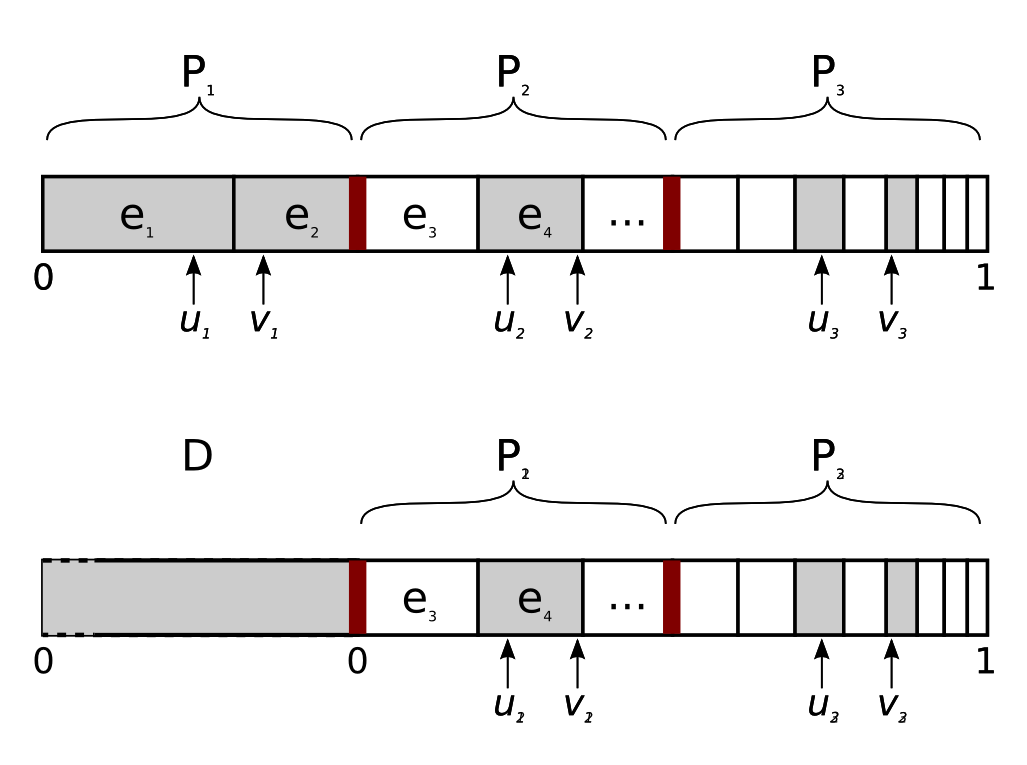
\includegraphics[width=0.9\columnwidth]{figures/pt2/move_to_deterministic}
		\caption{A REFAIRE NOTATION.............}
		\label{fig:move_to_deterministic}
		$E(I)$
	\end{center}
\end{figure}


\begin{figure}[h!]
	\begin{center}
		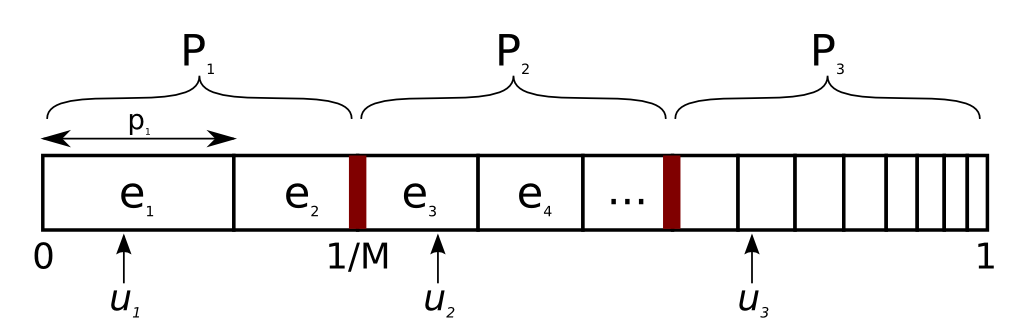
\includegraphics[width=0.9\columnwidth]{figures/pt2/comb}
		\caption{A REFAIRE NOTATION.............}
		\label{fig:comb}
		$E(I)$
	\end{center}
\end{figure}


\begin{figure}[h!]
	\begin{center}
		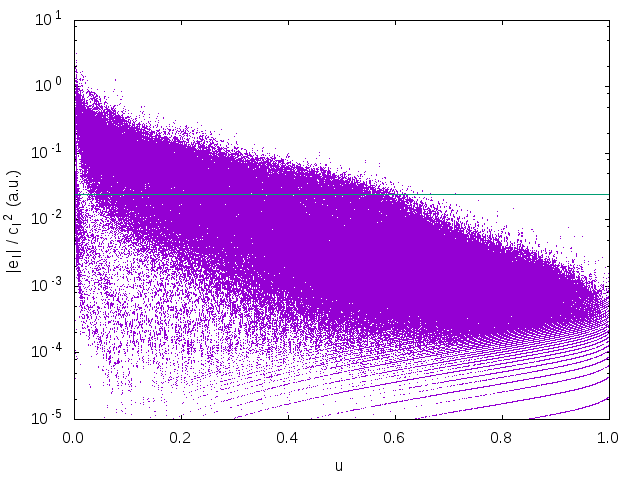
\includegraphics[width=0.9\columnwidth]{figures/pt2/eici2}
		\caption{A REFAIRE NOTATION.............}
		\label{fig:eici2}
		$E(I)$
	\end{center}
\end{figure}


\begin{figure}[h!]
	\begin{center}
		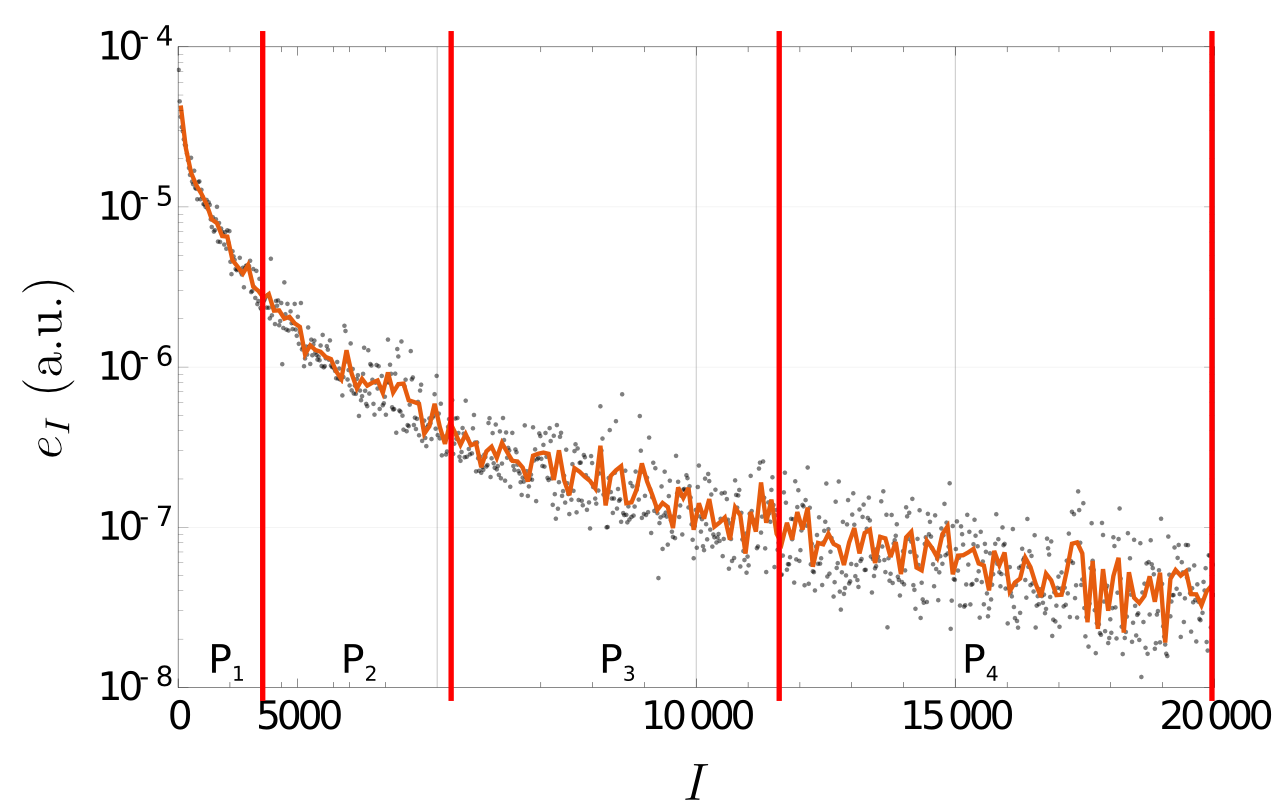
\includegraphics[width=0.9\columnwidth]{figures/pt2/P_i}
		\caption{A REFAIRE NOTATION.............}
		\label{fig:p_i}
		$E(I)$
	\end{center}
\end{figure}


\begin{figure}[h!]
	\begin{center}
		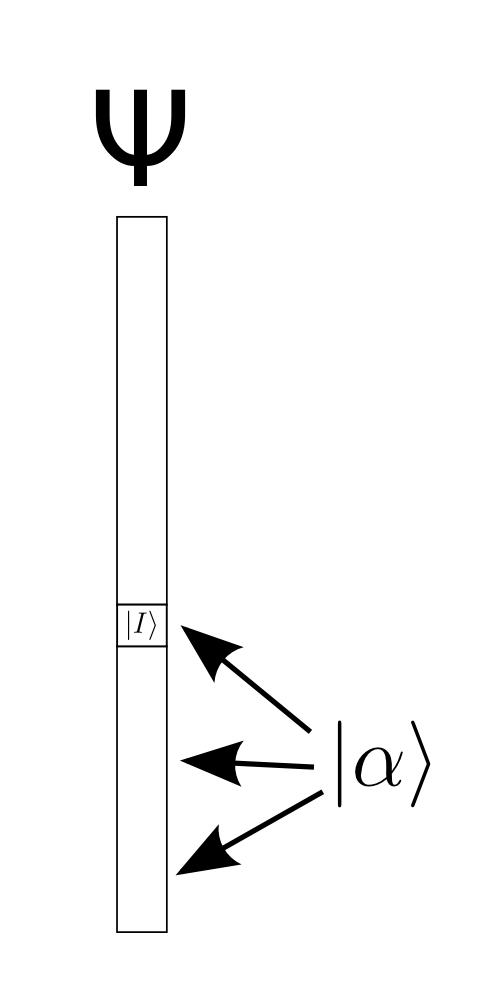
\includegraphics[width=0.2\columnwidth]{figures/pt2/a_con}
		\caption{A REFAIRE NOTATION.............}
		\label{fig:a_con}
		$\ket \alpha$ generated by increasing $\Psi_i$ connect to smaller and smaller norm of $\Psi$.
	\end{center}
\end{figure}

\begin{figure}[h!]
	\begin{center}
		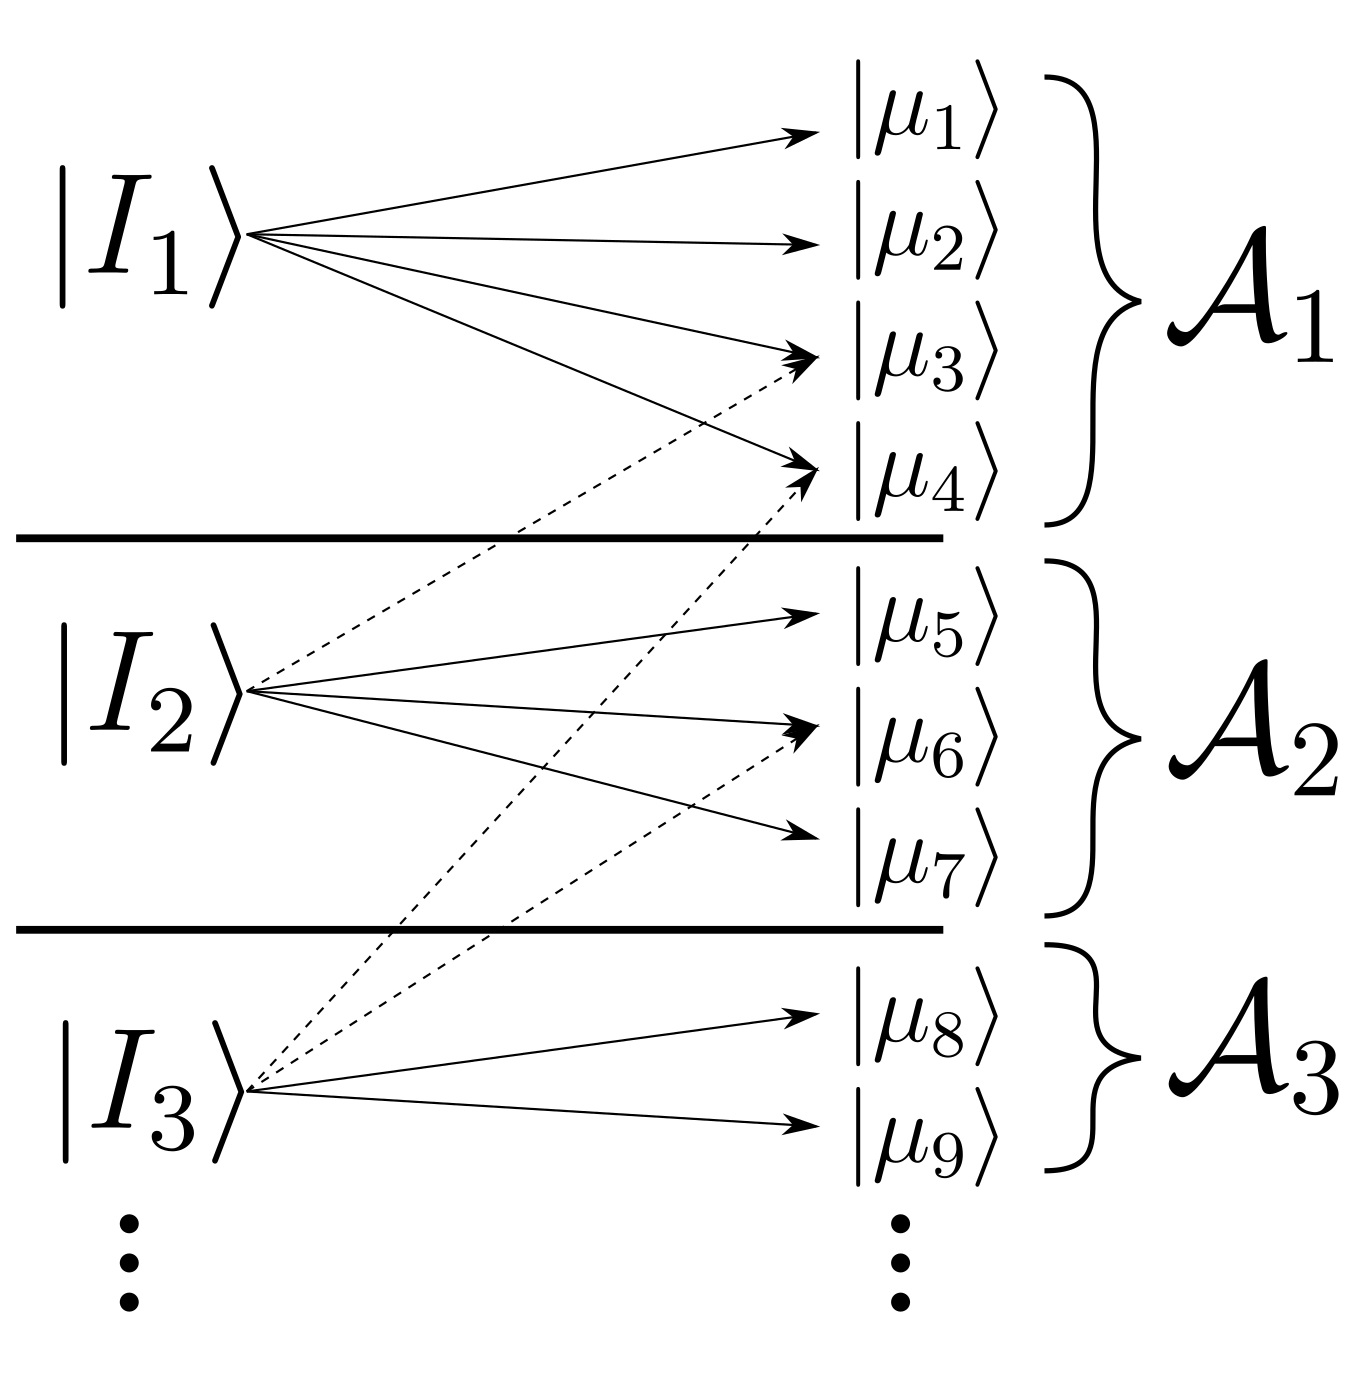
\includegraphics[width=0.5\columnwidth]{figures/pt2/mu_sample}
		\caption{}
		\label{fig:mu_sample}
		Construction of batches of $\ket \alpha$
	\end{center}
\end{figure}



\begin{figure}[h!]
	\label{comb_variables}
	\begin{center}
		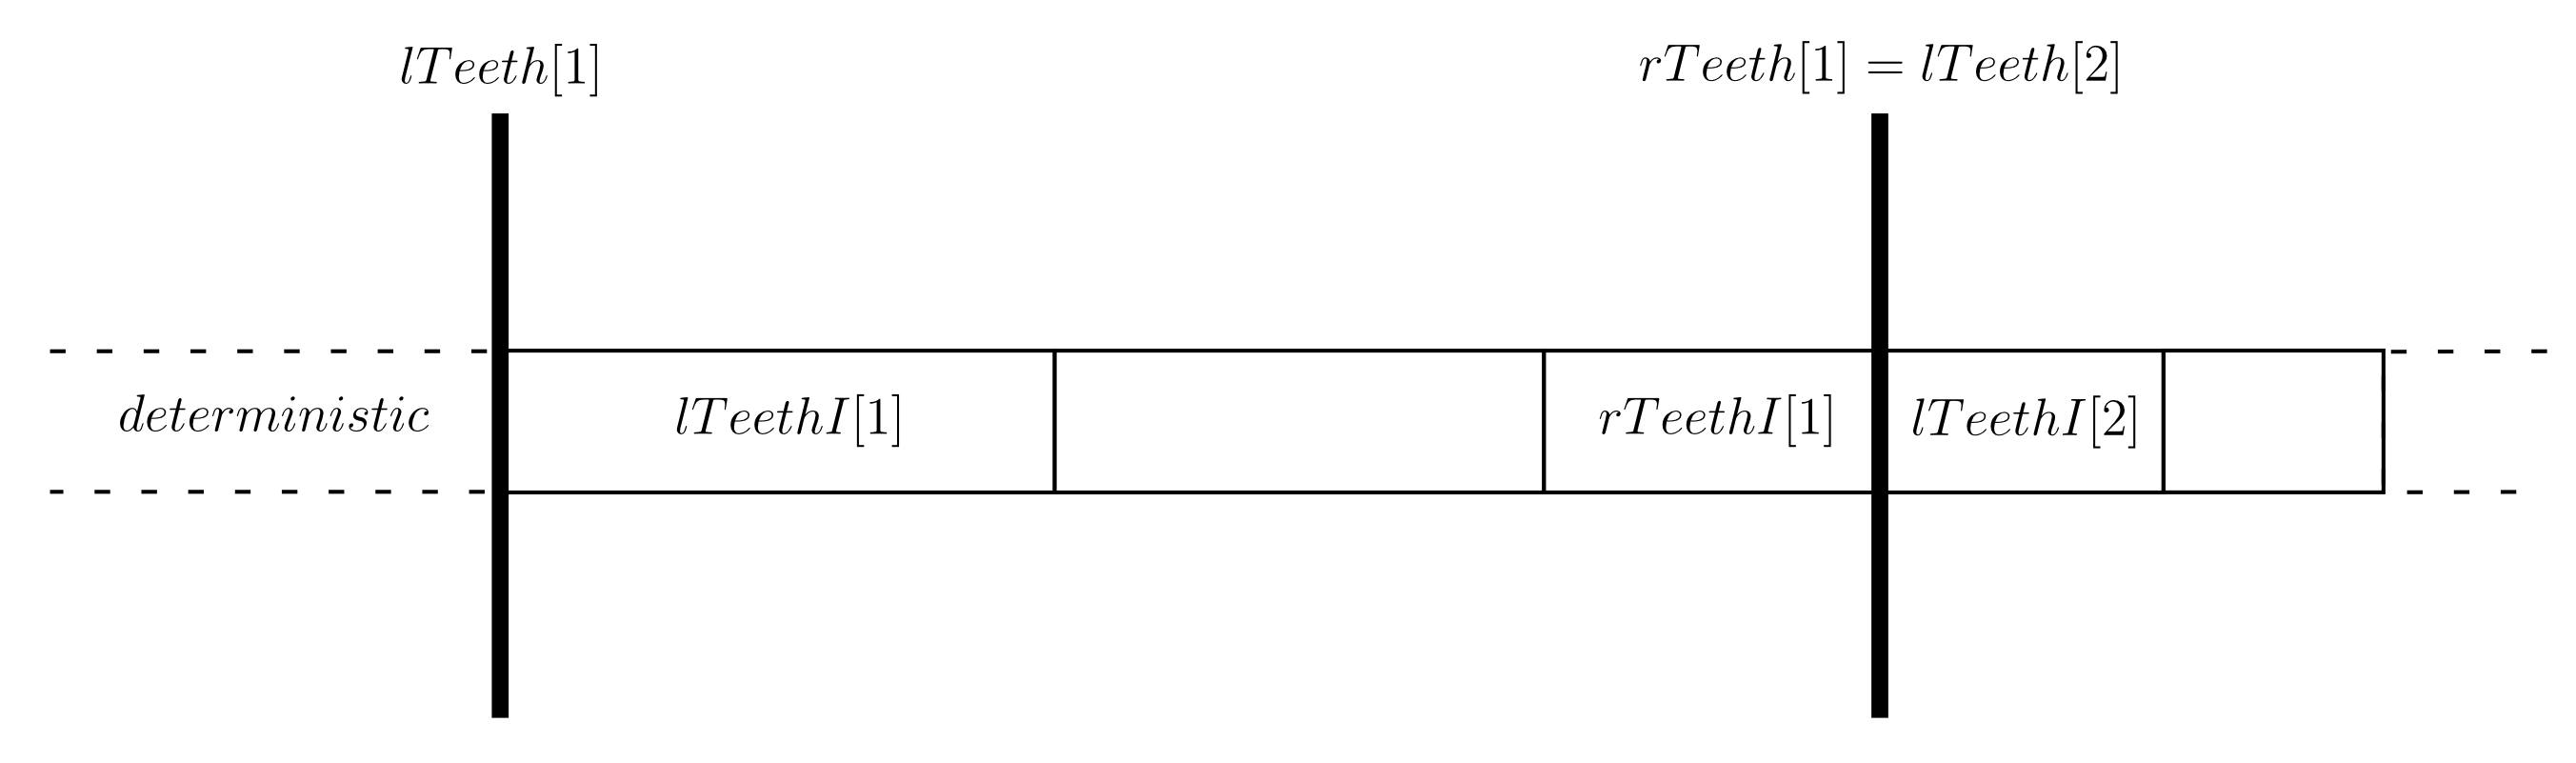
\includegraphics[width=1.00\columnwidth]{figures/pt2/teeth}
		\caption{comb}
		Variable names for the "comb" partition of $\Psi$. In boxes are shown indices, above are shown probabilities
		$$toothOfDet[i] = t ; i \in \big [ lTeethI[t],rTeethI[t] \big ]$$
		$$toothSize[t] = rTeeth[t] - lTeeth[t]$$
	\end{center}
\end{figure}

\begin{figure}[h!]
	\begin{center}
		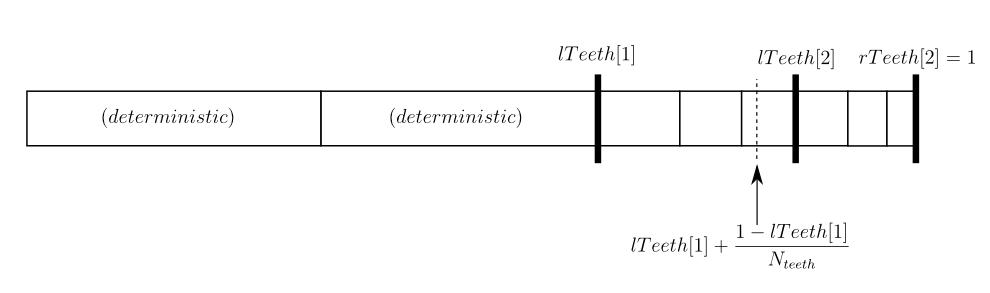
\includegraphics[width=1.00\columnwidth]{figures/pt2/teeths}
		\caption{\label{filtering}}
		Construction of teeth with $N_{teeth} = 2$ and 2 samples in the initial deterministic set.
	\end{center}
\end{figure}

\begin{figure}[h!]
	\begin{center}
		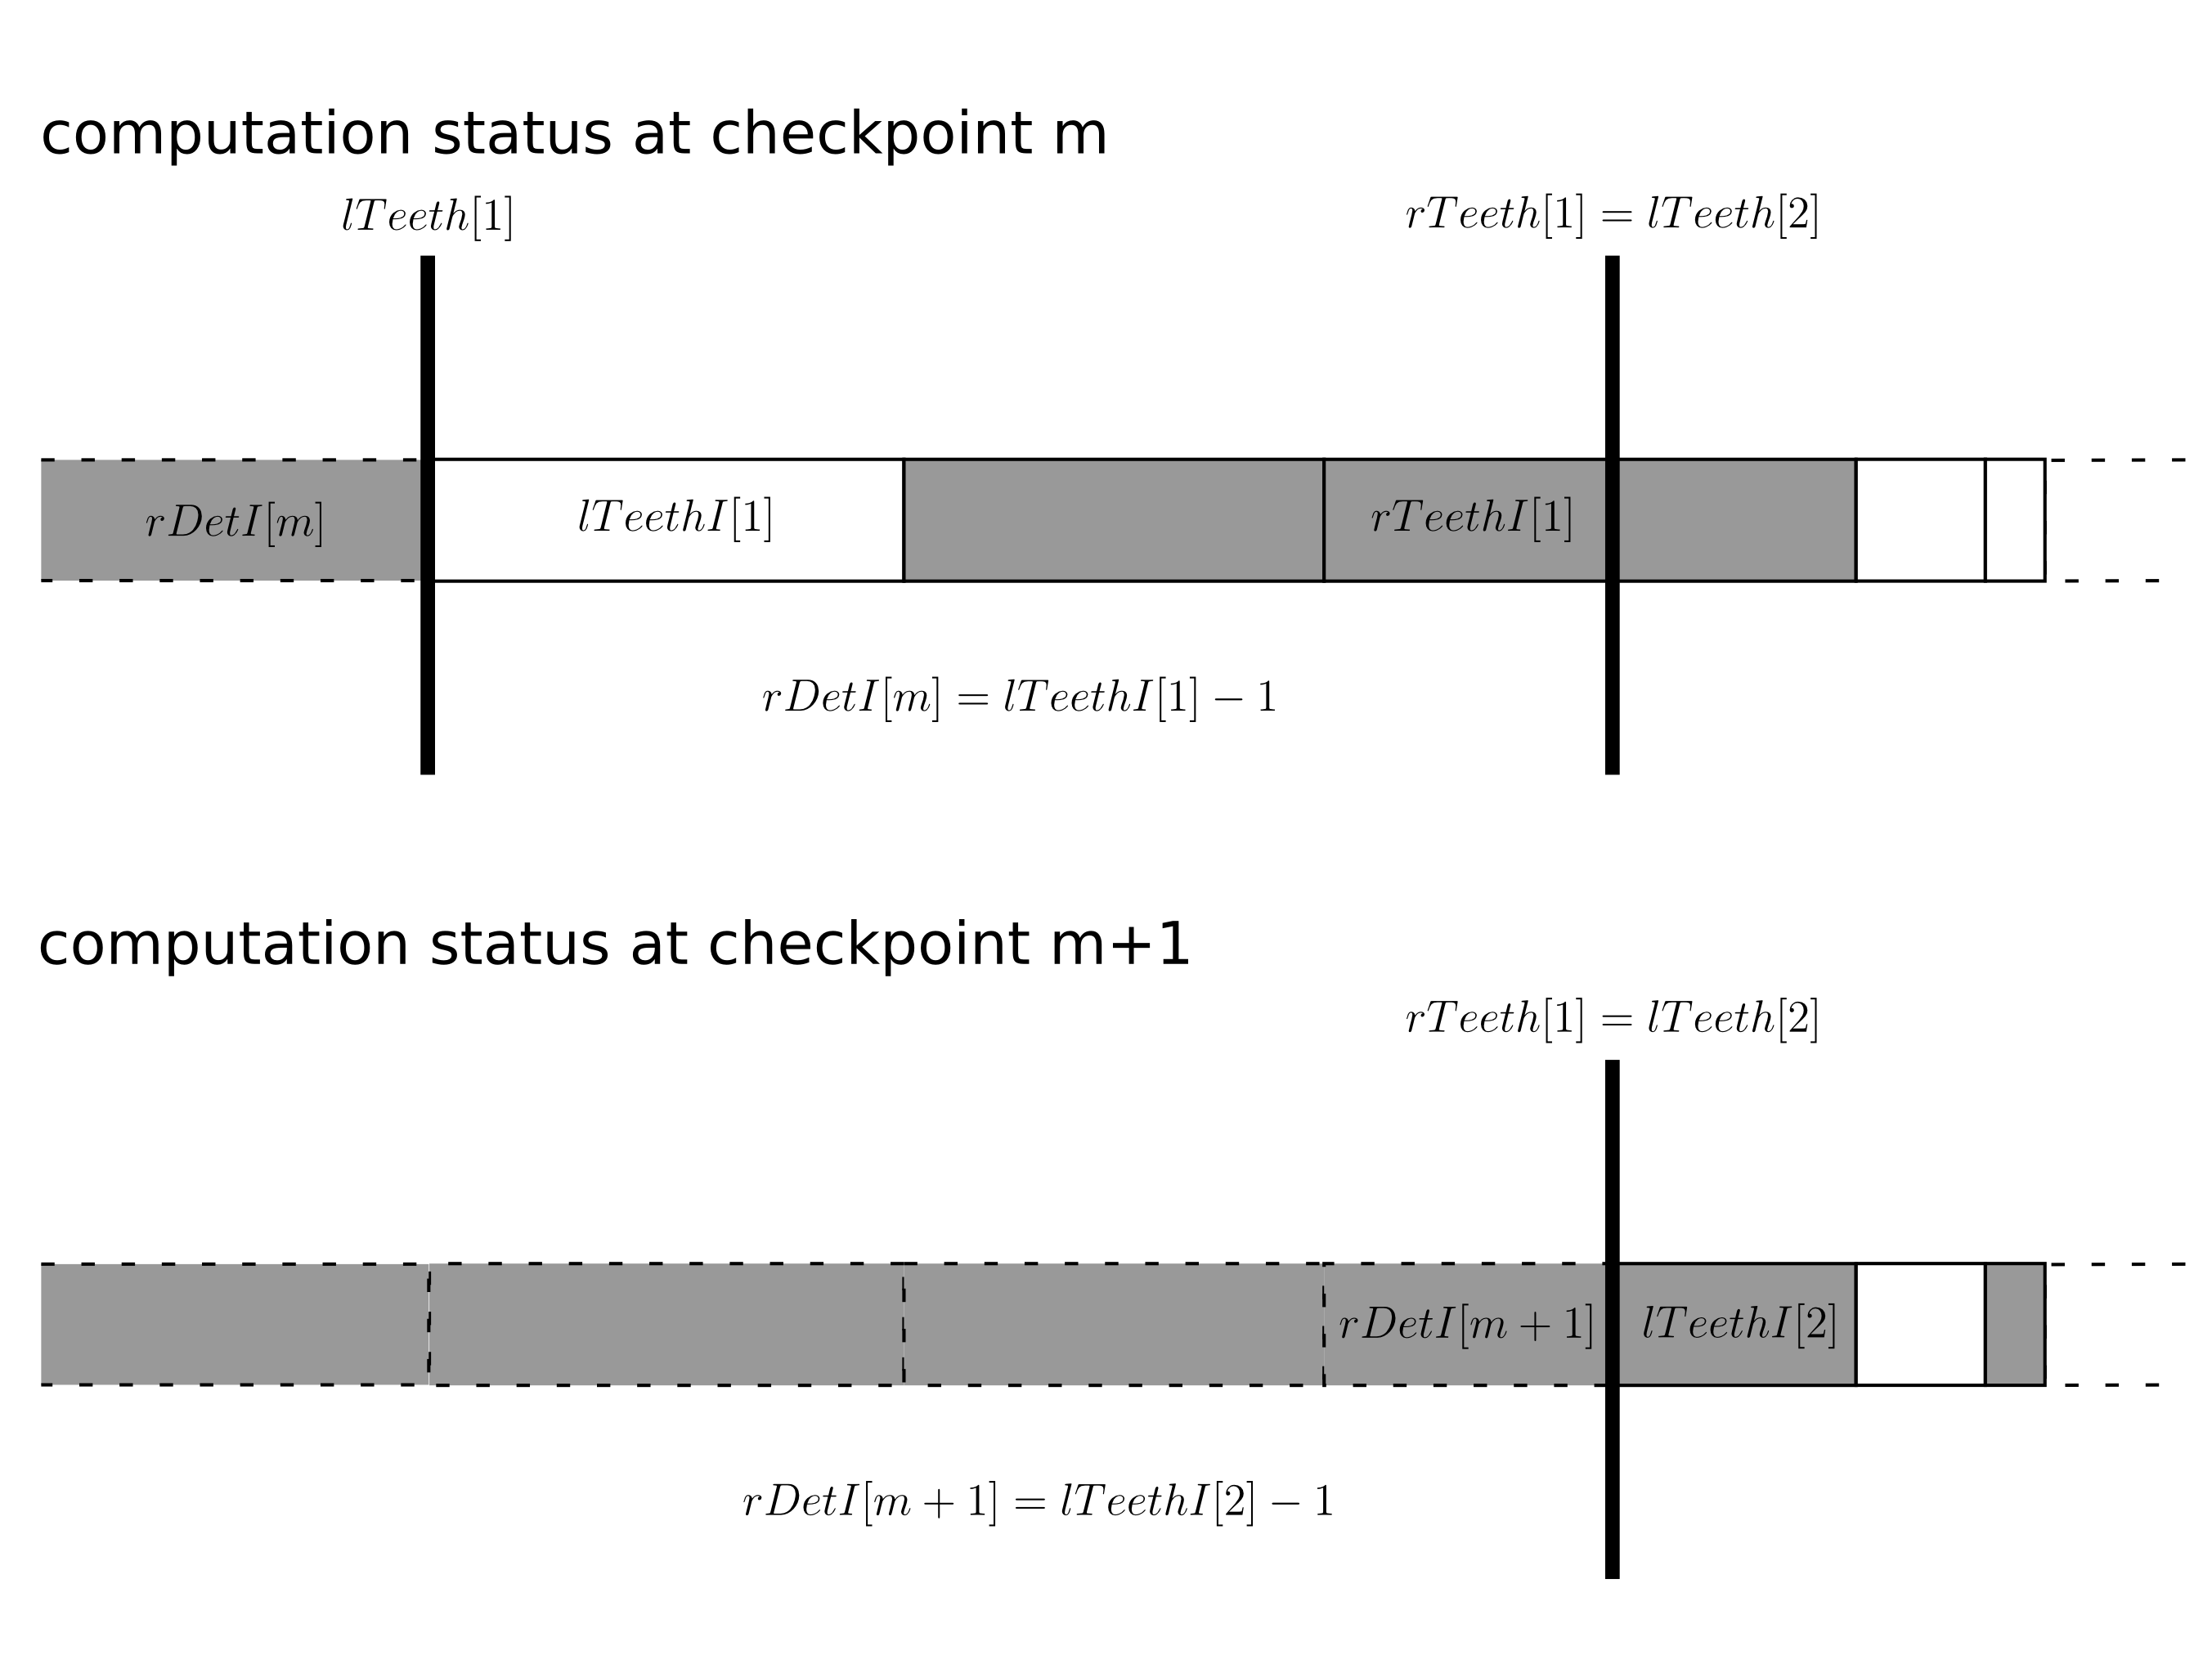
\includegraphics[width=1.00\columnwidth]{figures/matrix_dressing/deterministic_cp}
		\caption{\label{filtering}}
		$rDetI[m]$ gives the index of the last sample of the deterministic part at checkpoint $m$, or $0$ if there is no deterministic part.
		Greyed samples have been computed. Dotted samples are in the deterministic part. Sample $lTeethI[1]$ has been computed between checkpoints $m$ and $m+1$, resulting in tooth $1$ begin fully computed and thus moved into the deterministic part.
	\end{center}
\end{figure}

\end{document}



\chapter{Matrix dressing}
\minitoc
\documentclass[./thesis.tex]{subfiles}

 
\begin{document}

since alpha/alpha interactions are by design ignored, computation of a c\_alpha should only require knowledge of it's connection with internal space \\
SUPER costly done naively \\
list of connection supplied by QP \\
general mode \\
mircolist for connection \\
feuille de PQ to avoid duplicates \\
( custom buffers for more complex cases ) \\
repeated excitation mode(?)  \\
existing excitations are listed \\
alphas are generated through repeating excitations \\

microlisted \\
\section{def}
Idea is to create an external space and compute its influence on our selected space.
External space is only defined by c\_I\_alpha ; user should be able to only define that
By design, intern->extern and extern->extern influence isn't taken into account ( that's why it's called "external space"... )
Take into account c\_I\\alpha in the diagonalization of H : Matrix dressing
Matrix dressing
c\_I\\alpha may be derived from c ; in which case self-consistence/iteration


\section{implementation}
Plein de variable, subsection pour resumer la notation?
For clarity, indices will be named depending on what they refer to
\begin{itemize}
\item
$i,j$ refer to samples/generator determinants
\item
$m$ refers to checkpoints
\item
$t$ refers to teeth
\end{itemize}

In some respect, computing the dressing vector is akin to computing PT2. Matrix dressing can be seen as a sum of elementary dressing vectors $\delta_\alpha$, each one associated with a particular $\ket \alpha$, just like PT2 is a sum of $\epsilon(\alpha)$. It is possible to pack those elementary vectors together like we packed $\ket \alpha$ together for PT2.

\begin{equation}
\Delta_I = \sum_{\alpha \in \mathcal{A}_I} \delta_\alpha
\end{equation}


\begin{equation}
\Delta = \sum_{I} \Delta_I
\end{equation}

Thus, both are a sum over all external determinants, and require to find connections between those determinants and the internal wavefunction. Presumably, the norm of resulting elementary dressing vectors, will scale in a fashion similar to that of $E(I)$ ( je sais pu la notation )
With that in mind, is seems possible, theoritically, to generalize our hybrid stochastic-deterministic PT2 for computing dressing vectors.
However there are a few significant difference.
\begin{itemize}
\item
We were estimating a scalar, now we are estimating a vector. What should the error bar refer to?
\item
In both cases we have $N_{gen}$ samples, however for PT2 each sample is a scalar, here each sample is a vector size $N_{det}$. It is easy to store $N_{gen}$ scalars, not to store $N_{gen}$ vectors size $N_{det}$
\item
In the case of PT2 ( at least in it Epstein-Nesbet version ), each connection found, only requires an increment of some elements of $P(G_{pq})$. At no point 2 connections need to be known at the same time. This is different for methods implemented with matrix dressing( or even with other version of PT2? ). It is possible that the detail of which variational determinants a $\ket \alpha$ connects to, needs to be known in ordrer to be able to compute $delta_\alpha$.
\end{itemize}

To address the first problem, we decided to compute the error bar for $E_{\Delta}$ the energy contribution of $\Delta$. Our dressed matrix being $H + \Delta$, its energy is
    
\begin{equation}
\frac{\langle \Psi |H + \Delta | \Psi\rangle}{\langle \Psi | \Psi \rangle} = \frac{\langle \Psi |H  | \Psi\rangle}{\langle \Psi | \Psi \rangle} + \frac{\langle \Psi |\Delta | \Psi\rangle}{\langle \Psi | \Psi \rangle} = E_H + E_{\Delta} 
\end{equation}


$E_{\Delta}$ will be estimated just like we did for $E_{PT2}$. A vector size $N_{gen}$ is allocated to store individual $E_{\Delta_I}$.

\subsection{storage}

The core idea is that, in a Monte-Carlo scheme, even an "exotic" one like our own, the estimated result has to be a linear combination of all samples. At any point $m$ of the Monte-Carlo, corresponding to a number of samples being drawn, we can write our estimated dressing vector $\Delta^m$ as :


\begin{equation}
\Delta^m = \sum_{I=1}^{N_{gen}} \epsilon^m_{I} \Delta_I
\end{equation}


The values for $\epsilon^m_I$ have no dependence on those of $\Delta_I$. They only depend on what samples have been drawn so far. If we decide beforehand in what order samples are to be drawn, we can compute $\epsilon$ vector for any point of the Monte-Carlo before any sample has been computed. This allows us to set up predetermined "checkpoints".

\begin{figure}[h!]
	\begin{center}
		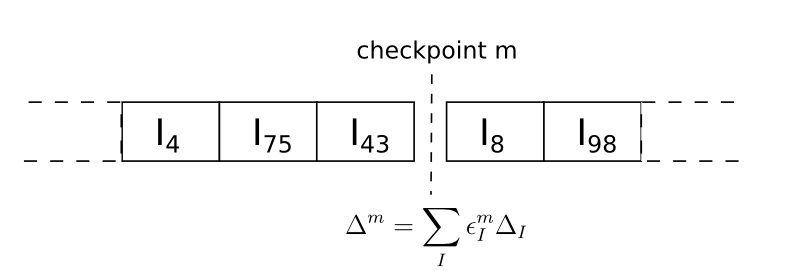
\includegraphics[width=1.00\columnwidth]{figures/matrix_dressing/checkpoint}
		\caption{\label{checkpoint}}
		CONFUSION ENTRE CHECKPOINT ET DENT POSSIBLE, RENDRE VERTICAL?
	\end{center}
\end{figure}


Those checkpoints can be set at any arbitrary point, but they must be determined beforehand and cannot be changed during the computation ; we will only be able to get results at those points.
For checkpoint $m$, we start with a null vector $\tilde \Delta^m$. Each time an elementary vector $\Delta_I$ is computed
we increment it 



\begin{equation}
\tilde \Delta^m \gets \tilde \Delta^m + \epsilon_I^m \Delta_I
\end{equation}


Once this has been done, $\Delta_I$ can be discarded. Indeed, when checkpoint $m$ is reached, $\tilde \Delta^m = \Delta^m$, as obviously $\epsilon_I^m = 0$ for any $\Delta_I$ sample that hasn't yet been drawn at $m$. ( preciser que c'est l'ordre de CALCUL pas de TIRAGE ).( VARIABLES DEFINI NORMALEMENT DANS LE CHAPITRE PT2... )

$\epsilon$ is defined as follow


\begin{equation}
acm[i] = \frac{toothSize[toothOfDet[i]]}{w[i]}
\end{equation}

%
\begin{equation}
acw[i] = \frac{teethSize[teethFromDet[i]]}{cm[i]-cm[i-1]};i>1
\end{equation}




\begin{equation}
\epsilon^m_i = \frac{acw[i] \times n[m,i]}{N[m]}  ; i>rDetI[m] ??
\end{equation}



\begin{equation}
\epsilon^m_i = 1 ; i \leq rDetI[m] ??
\end{equation}


The memory cost for a checkpoint $m$ is $2 \times N_{det}$ floats, corresponding to the storage of $\epsilon^m$ and $\tilde \Delta^m$. This cost is small enough to allow setting up quite a few checkpoints. However, in addition to this memory cost, comes some computational cost. If we set up $N_{cp}$ checkpoints, it implies each time a sample is drawn, we will have, theoretically, to incremement $N_{cp}$ vectors of size $N_{det}$. For quicker jobs, this price may not be negligible. It gets worse if, as was the case in our first implementations, a collector is in charge of updating checkpoints for multiple slaves. 


We can drastically reduce the amount of writting required for each sample, by separating the deterministic and stochastic part, and computing differences between checkpoints rather than checkpoints directly.
For the deterministic part, things are straightforward. We allocate a vector $\Delta^{D,t}$ of size $N_{det}$ for each tooth $t$, and one $\Delta^{D,0}$ for the initial deterministic set. For each sample that is computed, the $\Delta^{D,t}$ vector corresponding to the $t$ tooth it belongs in - or $\Delta^{D,0}$ if it belongs in the initial deterministic part - is incremented. That's exactly 1 vector write per sample.

For the stochastic part, instead of using $\epsilon$, we use $\tilde \epsilon$, defined as follow.


\begin{equation}
\tilde \epsilon^m_i = 0 ; i \leq rDetI[m]
\end{equation}



\begin{equation}
\tilde \epsilon^1_i = acw[1] \times n[1,i]  ; i>rDetI[1] ??
\end{equation}



\begin{equation}
\tilde \epsilon^m_i = acw[i] \times (n[m,i]-n[m-1,i])  ; i>rDetI[m]; m>1 ??
\end{equation}


(notation  $\tilde \Delta^m$ utilise aussi pour $\epsilon$ )
As can be seen, $\tilde \Delta^m$ will need to be updated when sample $i$ is computed, only if $(n[m,i]-n[m-1,i]) \neq 0$, in other word, only if $i$ has been drawn between checkpoint $m-1$ and $m$. [This means at most 1 writting ( instead of $N_{cp}$ ) each time a sample is drawn.]FAUX? 

$\epsilon$ can be reconstructed from $\tilde \epsilon$.




\begin{equation}
\epsilon^m_i = \frac{1}{N[m]} \sum_{j=1}^{m} {\tilde \epsilon^j_i} ; i > rDetI[m]
\end{equation}


\begin{equation}
\epsilon^m_i = 1; i \leq rDetI[m]
\end{equation}



$\epsilon^m_i$ is not explicitely reconstructed in the shown algorithms, $\Delta^m$ is directly computed from $\tilde \epsilon^m_i$.

FORMULE


\begin{algorithm}
	\caption{OPTIMIZE\_MONTECARLO}
	\label{OPTIMIZE_MONTECARLO}
	
	\SetKwFunction{FMain}{OPTIMIZE\_MONTECARLO}
	\SetKwProg{Fn}{Function}{:}{}
	
	\Fn(\tcc*[h]{Optional algorithm to reorder jobs so checkpoints are reached as fast as possible.}){\FMain{some args}}{
		$lastNj \gets 1$ \;
		\For{$m=1,N_{cp}$}{
			$Nmoved \gets 0$ \;
			\For{$j=lastNj,cpthreshold[m]$}{
				\If{$n[m,J_j] = 0 \& J_j > rDetI[m]$}{
					\tcc{ensures moved jobs are at the end of the checkpoint once sorted}
					$J_j \gets J_j + N_{gen}$ \;
					$Nmoved \gets Nmoved + 1$ \;
				}
			}
			sort array J from $lastNj$ to $cpthreshold[m]$, inclusive \;
			\tcc{moved jobs are sent to the next checkpoint}
			$cpthreshold[m] \gets cpthreshold[m] - Nmoved$ \;
			\tcc{restores moved jobs original value}
			\For{$j=cpthreshold[m]+1,cpthreshold[m] + Nmoved$}{
				$J_j \gets J_j - N_{gen}$ \;	
			}
			$lastNj \gets cpthreshold[m] + 1$ \;
		}
	}
\end{algorithm}

Algorithm (Nmoved) is an optional reorganization of jobs order. It doesn't change the result for any checkpoint, but only ensures it is available as quickly as possible. It takes two things into consideration:
\begin{itemize}
\item
Because no result is available between two checkpoints, the order in which jobs are processed between two checkpoints is irrelevant for the result. So, as is usually the case with parallel jobs, we would like to do the longest tasks first, so that we don't get an extra delay due to a massive task being done last. Therefore, jobs should always be in ascending order ( descending computational time N'A PAS ETE EXPLIQUÉ) between two checkpoints.
\item
Because of the "tooth filling", sometimes samples computed inside a checkpoint aren't useful for the result. Since tooth filling picks the first uncomputed jobs, they are of high computational cost. The algorithm iterates over checkpoints in ascending order, each time moving such sample to the next checkpoint. Thus, every sample is moved to the first checkpoint it's actually involved in, either deterministically or stochastically.
\end{itemize}



\begin{algorithm}
	\caption{PRECOMPUTE\_MONTECARLO}
	\label{PRECOMPUTE_MONTECARLO}
	\tcc*[h]{Computes $J$ the array so that $J_i$ is the $i^{th}$ sample that must be computed to perform the Monte-Carlo computation, and $n[m,i]$ the total number of times sample $i$ has been drawn at checkpoint $m$, regardless of which teeth are in the deterministic part.}
	
	\KwData{$cpthreshold[m]$ is the minimal number of jobs required to reach checkpoint $m$. It's updated to match the end of a comb ( pas clair? )}
	\KwData{$cpthreshold[N_{cpmax}] = N_{gen}$}
		$N_s \gets rDetI[1]$ \;
		$N_j \gets rDetI[1]$ \;
		\For{$i=1,N_j$}{
			$d_i \gets TRUE$ \;
			$J_i \gets i$ \;
		}
		
		$curcp \gets 1$ \;
		$curth \gets 1$ \;
		$U \gets N_j$ \;
		\While{$N_j < N_{gen}$}{
		  $ADD\_COMB($,$RANDOM[0,1]$,$J$, $N_j$, $d$, $n_g)$  \;
		  \While{$U < N_{gen}$}{
		    $U \gets U + 1$ \;
            \If{$not\ d_U$}{
              $d_U \gets TRUE$ \;
              $N_j \gets N_j+1$ \;
              $J_{N_j} \gets U$ \;
              break \;
            }
		  }
		  
		  $N_s \gets N_s + 1$ \;
		  $oldcurth \gets curth$ \;
		  \While{$curth \leq N_{cpmax}$}{
		  	\If{$N_j \leq cpthreshold[curth]$}{
		  		$curth \gets curth + 1$ \;
		  	}
		  }
		  
		  \If{$oldcurth \neq curth$}{

		    $cpthreshold[curcp] \gets N_j$ \;
            $n[curcp,*] = n_g[*]$ \;
            $N[curcp] = N_s$ \;
            $curcp \gets curcp+1$ \;	
		  } 
		}
		$N_{cp} = curcp - 1$ \;
	
\end{algorithm}



\begin{algorithm}
	\label{COMPUTE_EPSILON}
	\caption{COMPUTE\_EPSILON}
		%\KwData{ $I$ the bitstring representation of a determinant $D_I$}
		\KwResult{ $\tilde \epsilon$ as described ... quelque part}
		$\epsilon^*_* \gets 0$ \;
		$U \gets 1$ \;		
		\For{$m=1,N_{cp}$}{
			$lastTeeth[m] = 0$ \;
			$rDetI[m] = lTeeth[1]-1$ \;
			\While{$U \leq N_{gen}$}{
				\uIf{$n[m,U] \neq 0$}{
					$U \gets U+1$ \;
				}\Else{
					break \;
				}
		  	}
			\For{$t=N_{teeth},1,step=-1$}{
				\If{$U-1 \leq rTeethI[t]$}{
					$lastTeeth[m] = t$ \;
					$rDetI[m] =rTeethI[t]$ \;
					break loop \;
				}
			}
			
			
			\For{$t=lastTeeth[m]+1,N_{teeth}$}{
				\For{$i=lTeethI[t],rTeethI[t]$}{
					$\tilde \epsilon^m_i \gets \frac{toothSize[t] \times n[m,i]}{w[i]}$ \;
				}
			}
		}
		\For{$m=N_{cp},2,step=-1$}{
			$\tilde \epsilon^m_* \gets \tilde \epsilon^m_* - \tilde \epsilon^{m-1}_*$ \;
		}
\end{algorithm}

\begin{algorithm}
	\label{UPDATE_CHECKPOINT}
	\caption{UPDATE\_CHECKPOINT}
		%\tcc{updates checkpoint $i_{cp}$ - ERREUR SUR $\sigma^2$$}
		
		\SetKwFunction{FUpdateCheckpoints}{UpdateCheckpoints}
		\SetKwProg{Fn}{Function}{:}{}
	
		\Fn(\tcc*[h]{Update checkpoints when a sample is computed}){\FUpdateCheckpoints{}}{
			$contrib \gets \delta_I \cdot C$ \;
			$t \gets teethOfDet[I]$ \;

			

				$\Delta^{D,t} \gets \Delta^{D,t} + \delta_I$ \;

		\For{$m=1,N_{cp}$}{
			$\sigma[m] += n(m,I) \times contrib$ \;
			$\sigma_2[m] += n(m,I) \times contrib^2$ \;
			$\tilde \Delta^{m} \gets \tilde \Delta^{m} + n(m,I) \times \Delta_I$ \;
		}
		}
		
\end{algorithm}
\begin{algorithm}
	\label{COMPUTE_CHECKPOINTS}
	\caption{COMPUTE\_CHECKPOINTS}
		\tcc{result for checkpoint $i_{cp}$}
		
		\SetKwFunction{FComputeCheckpoints}{ComputeCheckpoints}
		\SetKwProg{Fn}{Function}{:}{}
	
		\Fn(\tcc*[h]{Compute the final estimated dressing vector}){\FComputeCheckpoints{some args}}{
			%$\Delta^m \gets \Delta_{deterministic}$\;
			\For{$t=0,lastTeeth[m]$}{
				$\Delta^m \gets \Delta^m + \Delta^{D,t}$ \;
			}
			\For{$m'=1,m$}{
				$\Delta^m \gets \Delta^m + \frac{\tilde \Delta^{m'}}{N[m]}$
			}
		}
\end{algorithm}



\subsection{finding connections - microlists}

For merely enumerating the connections between internal and external space, there are two possible ways.
Internal to external, or External to internal
%\begin{figure}[h!]
	\begin{center}
		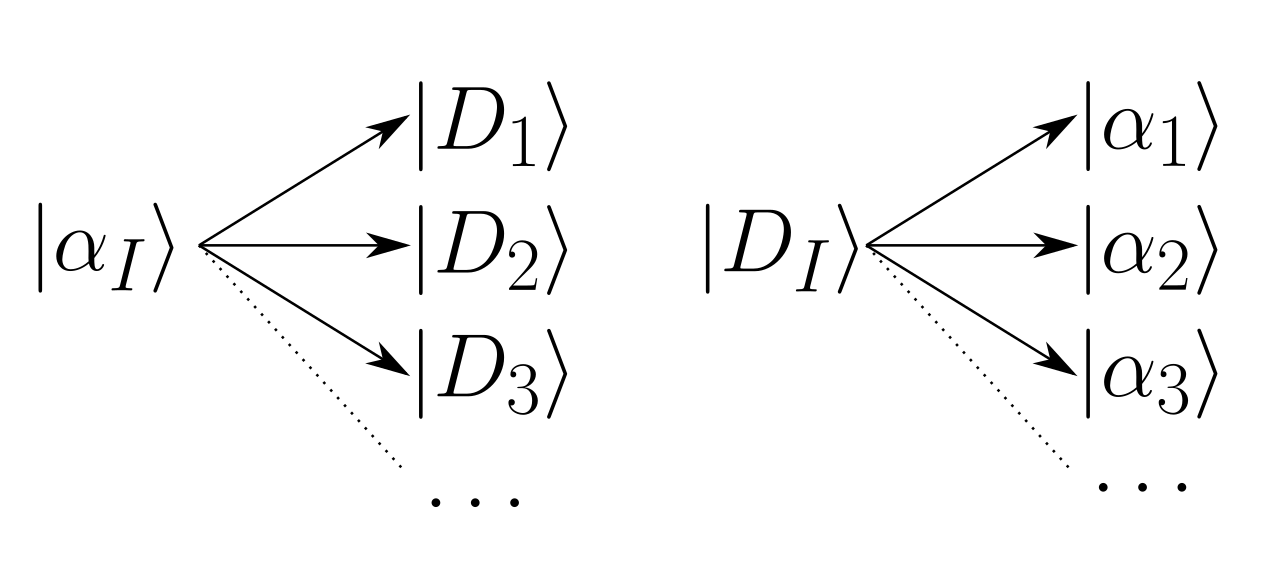
\includegraphics[width=0.5\columnwidth]{figures/matrix_dressing/interactions}
		%\caption{\label{interactions}}
	\end{center}
%\end{figure}

Computation-wise, those two possbilities are very different.

The internal to external approach is pretty straightforward, as it means applying every possible double excitation to all determinants of an arbitrary set $\Psi$ of size $N_{det}$. The only difficulty is to ensure the created $\alpha$ are actually external to $\Psi$. We did this and more in our CIPSI implementation.

The external to internal approach is more difficult as it means finding connections between all determinant $\alpha$ in an arbitrary set size $N_{external}$ - typically a few orders of magnitude larger than $N_{det}$ - and a set of abritrary determinants $\Psi$. 

Unfortunately, we typically need to know all connection for a particular $\alpha$ before we can compute its associated dressing vector, which puts us in the internal to external case.

In our CIPSI algorithm, we are only considering $N_{virt}^2$ $\alpha$ at the same time. We can build, for each of those $\alpha$, a list of connected $I$ that we incrementally build from connections we find by internal-to-external approach.


However, the storage space for the worst-case scenario isn't sustainable. ( a reformuler/clarifier ptet)
$G_{pq}$ being the first batch, and the variational wavefuction being all determinants up to quadruply excited from $G$ except those in the $G_{pq}$ batch. There are $~ N_{virt}^2$ unique $\alpha$ in the batch. For each of them, any of the $~N_{occ}^2 N_{virt}^2$ double excitation will lead to a variational determinant, except if it leads to one of the $N_{virt}^2$ determinant of the batch.
We have $~ N_{virt}^2$ alpha each connected to $~(N_{occ}^2-1) N_{virt}^2$ variational determiants, resulting in a storage space $~N_{occ}^2 N_{virt}^4$.
Even in the more realistic case where half of double excitations involving the holes in the HOMO of the HF determinants are present in the internal space, storage needed for the ionzied generator $a_{\bar{HOMO}} a_{HOMO} HF$ will be $N_{virt}^4 / 4$, which, depending on the system size, may be concerningly or prohibitively high. 

(PREUVE?)

\begin{algorithm}
	\label{BUILD_CONNECTED}
	\caption{BUILD\_CONNECTED}
		\KwData{ ---------}
		\KwResult{ ------------}
        $i_1 = N$ \;   
        $L_{1..i_1} \gets D_{1..{i_1}}$ \;
		\ForAll{$r ; B_{r0}$}{
		\tcc {$B_{r0} = FALSE$ if column entirely tagged}
		  $i_2 = i_1 + N^r$ \;
		  $L_{i_1+1..i_2} \gets D^r_{1..N^r}$ \;
		  \For{$i=1,N_r$}{
		    $T_{D^r_i} \gets FALSE$
		  }
		  \ForAll{$s ; B_{s0}$}{
		    $i_3 = i_2$ \;
		    \For{$i=1,N_s$}{
		      \If{$T_{D^s_i}$}{
		        $i_3 \gets i_3+1$ \;
		        $L_{i_3} \gets D^s_i$ \;
		      }
		    }
		    
		    $i_4 = i_3 + N^{rs}$ \;
		    $L_{i_3+1 .. i_4} \gets D^{rs}_{1..N^{rs}}$ \;
		    \tcc{$L$ is the list of all $I \in \Psi ; EXC(I, a^\dagger_r a^\dagger_r G_{pq} ) \leq 2$}
		  }
		 \For{$i=1,N_s$}{
		    $T_{D^r_i} \gets TRUE$
		  }
		}
\end{algorithm}



\begin{algorithm}
	\label{BUILD_MICROLIST}
	\caption{BUILD\_MICROLIST}
		\KwData{ ------}
		\KwResult{ ------}
        $N \gets 0$ \;
        $N^* \gets 0$ \;   
        $N^{*,*} \gets 0$ \;    
        \ForAll{$I \in \{S - past\} ; f_{G_{pq}}^I \leq 4$}{
          $(P,H) \gets particles\_and\_holes(G_{pq}, I)$ \;
          $p = list\_from\_bitstring(P)$ \;
          
          %$h = LIST_FROM_BITSTRING(H)$
          \uIf{$f_{G_{pq}}^I = 4$ \& $B_{p_1,p_2}$}{
            $i \gets N^{p_1, p_2}+1$ \;
            $N^{p_1, p_2} \gets i$ \;
            $D^{p_1, p_2}_{i} \gets I$ \;
          }
          \uElseIf{$f_{G_{pq}}^I = 3$ \& $B_{p_1}$}{
            $i \gets N^{p_1}+1$ \;
            $N^{p_1} \gets i$ \;
            $D^{p_1}_{i} \gets I$ \;
          }
          \Else{
            $i \gets N+1$ \;
            $N \gets i$ \;
            $D_{i} \gets I$ \;
          }
        }
\end{algorithm}




\section{Alpha-factory (rename?)}


General framework which allows to create methods with minimal effort 

\section{parallel}
just like pt2 stoch, 1 task = 1 generator \\
however, 1 result = 1 vector instead of 1 scalar \\
additional difficulties \\
memory: \\
to avoid N\_det\^2, checkpoints \\
communication \\
4 scalars per checkpoint \\



\end{document}



\chapter{exponential dressing etc}
\documentclass[./thesis.tex]{subfiles}

 
\begin{document}

\begin{algorithm}
\KwData{$\kalpha$ the considered exernal determinant}
\KwData{$D_i$ the list of $N$ internal determinants connected to $\kalpha$}
\KwResult{finds all diamonds in $\mathcal{O}(N_{ref} \times N)$} 

\ForAll{$\kI$ with $EXC(\kI, \kalpha) \leq 4$}{

$\delta \gets -(I + \alpha)$ \;
$i \gets 1$ \;
$j \gets 1$ \;
\While{$j \leq N \wedge i \leq N$}{
	\uIf{$D_j - D_i > \delta$}{
		increment $i$ \;
	}
	\uElseIf{$D_j - D_i < \delta$}{
		increment $j$ \;
	}
	\Else
	{
		\tcc{$\hat T_{I \rightarrow D_j}$ is $D_j-I$}
		\tcc{$D_i + (D_j-I) = \alpha$}
		
		
		
		%\tcc{\alert{check diamond}}
		%\If{$(I \oplus D_i \wedge I = D_j \oplus \alpha \wedge D_j) \wedge (I \oplus D_i \wedge D_i = D_j \oplus \alpha \wedge \alpha)$}{
		%\If{$\hat T_{I \rightarrow D_i} = \hat T_{D_j \rightarrow \alpha}$}{
		
		\tcc{\alert{check if addition applies correct excitaion}}
		\tcc{impossible exciation results in an abnormal number of modified spinorbitals}	
		\If{$||D_j \oplus I|| = ||D_i \oplus \alpha||$}{
			diamond found \;
		}
		increment $i$ and $j$ \;
	}
}
}
\end{algorithm}

Applying an impossible excitation by addition, will usually lead to an abnormal result with a wrong number of ``electrons''. But in some cases, it may lead to an existing determinant. 



This algorithm works when bitstrings are considered binary integers of arbitrary size. However, no assumption is made about the operators involved in the diamond, they can be any combination of creations and anihilations. Therefore, for simplification purpose, it is possible to consider all 64-bit integers independently, each one carrying a subset of the operators involved in the excitation.

Essentially, adding and substracting can be done integer-wise, without the added complexity of carry and overflow.
Because integers of lower $\Nint$ vary more, they should be given more weight when comparing(???)



\begin{algorithm}
	\KwData{$I[]$ the children of $\kI$}
	
	\ForAll{$\ket {G_p}$ singly ionized generator}{
		\tcc{indexed by 1 hole and 2 particles}
		$c_\alpha[h,p1,p2]$ \;
		\tcc{$\kalpha = a_h a^\dagger_{p1} a^\dagger_{p2} \ket {G_p}$}
		\ForAll{$I,I[r],I[s]$}{
			$\alpha \gets I \oplus I[r] \oplus I[s]$ \;
			\tcc{check $||\alpha||$ ?}
			$x \gets G_p \oplus \alpha$ \;
			\If{$||x|| = 3$}{
				$(h,p1,p2) \gets \texttt{BITSTRING\_TO\_LIST}(x)$ \;
				increment $c_\alpha[h,p1,p2]$ \;		
			}
		}
	}
\end{algorithm}

\end{document}






\bibliographystyle{plain}
\bibliography{references}
\end{document}




